%-------------------------------------------------------------------------------
%                      Template Naskah Skripsi
%               	Berdasarkan format JTETI FT UGM
% 						(c) @gunturdputra 2014
%-------------------------------------------------------------------------------

%Template pembuatan naskah skripsi.
\documentclass{jtetiskripsi}

%Untuk prefiks pada daftar gambar dan tabel
\usepackage[titles]{tocloft}
\renewcommand\cftfigpresnum{Gambar\  }
\renewcommand\cfttabpresnum{Tabel\   }

%Untuk hyperlink dan table of content
\usepackage[hidelinks]{hyperref}
\newlength{\mylenf}
\settowidth{\mylenf}{\cftfigpresnum}
\setlength{\cftfignumwidth}{\dimexpr\mylenf+2em}
\setlength{\cfttabnumwidth}{\dimexpr\mylenf+2em}

%Untuk Bold Face pada Keterangan Gambar
\usepackage[labelfont=bf]{caption}

%Untuk caption dan subcaption
\usepackage{caption}
\usepackage{subcaption}

%pdf
\usepackage{pdfpages}

%table
\usepackage{array}
\usepackage{longtable}
\newcolumntype{P}[1]{>{\centering\arraybackslash}p{#1}}
\usepackage{graphics}
\usepackage{wrapfig}
% \usepackage{multirow}

%bibliography
\usepackage[
  style=authoryear-icomp,
  maxcitenames=1,
  isbn=false,
  doi=false,
  url=false,
  autolang=other,
  hyperref=true,
  sortcites=true,
  bibwarn=true,
  firstinits=true,
  autolang=other,
]{biblatex}
\DefineBibliographyStrings{english}{%
  andothers = {dkk\adddot,\addspace},
}
\DeclareFieldFormat{citehyperref}{%
  \DeclareFieldAlias{bibhyperref}{noformat}% Avoid nested links
  \bibhyperref{#1}}

\DeclareFieldFormat{textcitehyperref}{%
  \DeclareFieldAlias{bibhyperref}{noformat}% Avoid nested links
  \bibhyperref{%
    #1%
    \ifbool{cbx:parens}
      {\bibcloseparen\global\boolfalse{cbx:parens}}
      {}}}

\savebibmacro{cite}
\savebibmacro{textcite}

\renewbibmacro*{cite}{%
  \printtext[citehyperref]{%
    \restorebibmacro{cite}%
    \usebibmacro{cite}}}

\renewbibmacro*{textcite}{%
  \ifboolexpr{
    ( not test {\iffieldundef{prenote}} and
      test {\ifnumequal{\value{citecount}}{1}} )
    or
    ( not test {\iffieldundef{postnote}} and
      test {\ifnumequal{\value{citecount}}{\value{citetotal}}} )
  }
    {\DeclareFieldAlias{textcitehyperref}{noformat}}
    {}%
  \printtext[textcitehyperref]{%
    \restorebibmacro{textcite}%
    \usebibmacro{textcite}}}
\addbibresource{daftar-pustaka.bib}

%equation
\usepackage{amsmath}

%algorithm & syntax
\usepackage{algorithm}
\usepackage{algpseudocode}
\algnewcommand\algorithmicforeach{\textbf{for each:}}
\algnewcommand\ForEach{\item[ \algorithmicforeach]}
\algdef{SE}[DOWHILE]{Do}{doWhile}{\algorithmicdo}[1]{\algorithmicwhile\ #1}%
\newenvironment{conditions}
  {\par\vspace{\abovedisplayskip}\noindent\begin{tabular}{>{$}l<{$} @{${}={}$} l}}
  {\end{tabular}\par\vspace{\belowdisplayskip}}

\algdef{SE}% flags used internally to indicate we're defining a new block statement
[STRUCT]% new block type, not to be confused with loops or if-statements
{Struct}% "\Struct{name}" will indicate the start of the struct declaration
{EndStruct}% "\EndStruct" ends the block indent
[1]% There is one argument, which is the name of the data structure
{\textbf{struct} \textsc{#1}}% typesetting of the start of a struct
{\textbf{end struct}}% typesetting the end of the struct

%code
\usepackage{listings}
\usepackage{xcolor}
\definecolor{codegreen}{rgb}{0,0.6,0}
\definecolor{codegray}{rgb}{0.5,0.5,0.5}
\definecolor{codepurple}{rgb}{0.58,0,0.82}
\lstdefinestyle{mystyle}{
    commentstyle=\color{codegreen},
    keywordstyle=\color{magenta},
    numberstyle=\tiny\color{codegray},
    stringstyle=\color{codepurple},
    basicstyle=\ttfamily\footnotesize,
    frame=single,
    breakatwhitespace=false,
    breaklines=true,
    captionpos=b,
    keepspaces=true,
    numbersep=5pt,
    showspaces=false,
    showstringspaces=false,
    showtabs=false,
    tabsize=2
}
\lstset{style=mystyle}
\makeatletter
\def\thechapter{\@Roman\c@chapter}
\AtBeginDocument{%
  \def\thelstlisting{\@arabic\c@chapter.\@arabic\c@lstlisting}}
\makeatother


%-----------------------------------------------------------------
%Disini awal masukan untuk data proposal skripsi
%-----------------------------------------------------------------
\titleind{Improvisasi Crawling pada Peta Web Menggunakan
Algoritma Terdistribusi dengan Model Koordinasi Berbasis
Socket Programming}

\fullname{Muhammad Ridho Rizqillah}

\idnum{1313619033}

\approvaldate{10 Januari 2024}

\degree{Sarjana Ilmu Komputer}

\yearsubmit{2024}

\program{Ilmu Komputer}

\dept{Ilmu Komputer}

\firstsupervisor{Muhammad Eka Suryana, M. Kom.}
\firstnip{198512232012121002}

\secondsupervisor{Med Irzal, M. Kom.}
\secondnip{197706152003121001}

%-----------------------------------------------------------------
%Disini akhir masukan untuk data proposal skripsi
%-----------------------------------------------------------------

\tolerance=1
\emergencystretch=\maxdimen{}
\hyphenpenalty=10000
\hbadness=10000

\begin{document}

\cover{}
%-----------------------------------------------------------------

%-----------------------------------------------------------------
%Disini akhir masukan untuk muka skripsi
%-----------------------------------------------------------------
% \chapter*{\centering{\large{LEMBAR PERNYATAAN}}}
\onehalfspacing{}

Saya menyatakan dengan sesungguhnya bahwa skripsi dengan judul
\textbf{"Improvisasi Crawling pada Peta Web Menggunakan Algoritma Terdistribusi dengan Model Koordinasi Berbasis Socket Programming"} yang disusun sebagai syarat untuk memperoleh gelar Sarjana Komputer
dari Program Studi Ilmu Komputer Universitas Negeri Jakarta adalah karya ilmiah
saya dengan arahan dari dosen pembimbing.

Sumber informasi yang diperoleh dari peneliti lain yang telah dipublikasikan 
yang disebutkan dalam teks Skripsi ini, telah dicantumkan dalam Daftar Pustaka 
sesuai dengan norma, kaidah dan etika penulisan ilmiah.

Jika dikemudian hari ditemukan sebagian besar skripsi ini bukan hasil karya saya 
sendiri dalam bagian-bagian tertentu, saya bersedia menerima sanksi pencabutan 
gelar akademik yang saya sanding dan sanksi-sanksi lainnya sesuai dengan 
peraturan perundang-undangan yang berlaku.

\vspace{4cm}

\begin{tabular}{p{7.5cm}c}
	&Jakarta, 12 Januari 2024\\
	&\\
	&\\
	&\\
	&Muhammad Ridho Rizqillah
\end{tabular}

% \chapter*{\centering{\large{LEMBAR PERSETUJUAN}}}
\thispagestyle{empty} {\bf }Dengan ini saya mahasiswa Fakultas
Matematika dan Ilmu Pengetahuan Alam, Universitas Negeri Jakarta

\vskip3mm

\begin{tabular}{ll}
  Nama & : Muhammad Ridho Rizqillah \\
  No. Registrasi & : 1313619033 \\
  Program Studi & : Ilmu Komputer \\
  Judul & : Improvisasi Crawling pada Peta Web Menggunakan \\ & \hspace{0.2cm}
  Algoritma Terdistribusi dengan Model Koordinasi Berbasis \\ & \hspace{0.2cm}
  Socket Programming
\end{tabular}

\vskip3mm

\noindent \hskip10mm Menyatakan bahwa skripsi ini telah siap diajukan untuk sidang skripsi.
%\begin{center}
%Menyatakan bahwa skripsi ini telah siap diajukan untuk sidang skripsi.
%\end{center}



\begin{center}
\vskip3mm

Menyetujui,

\vskip3mm
\begin{spacing}{1.25}

\begin{tabular}{ccc}
  \hskip-2mm Dosen Pembimbing I & \qquad \qquad \qquad \qquad \qquad & \hskip-6mm Dosen Pembimbing II \\
   &  &  \\
   &  &  \\
   &  &  \\
   &  &  \\
  \hskip-2mm \underline{\textbf{Muhammad Eka Suryana, M.Kom}} &  & \hskip-6mm \underline{\textbf{Med
  Irzal, M.Kom}} \\
  \hskip-2mm NIP. 19770615 200312 1 001 &  & \hskip-6mm NIP. 19851223 201212 
  1 002	 \\
\end{tabular}
\end{spacing}
\end{center}
\vskip3mm
\begin{center}
Mengetahui, \\
Koordinator Program Studi Ilmu Komputer
\end{center}
\begin{spacing}{1.25}
{ \ }
\\
\\
{ \ }\begin{center}
\underline{\textbf{Dr. Ria Arafiyah, M.Si}} \\
{NIP. 19751121 200501 2 004}
\end{center}
\end{spacing} 

% 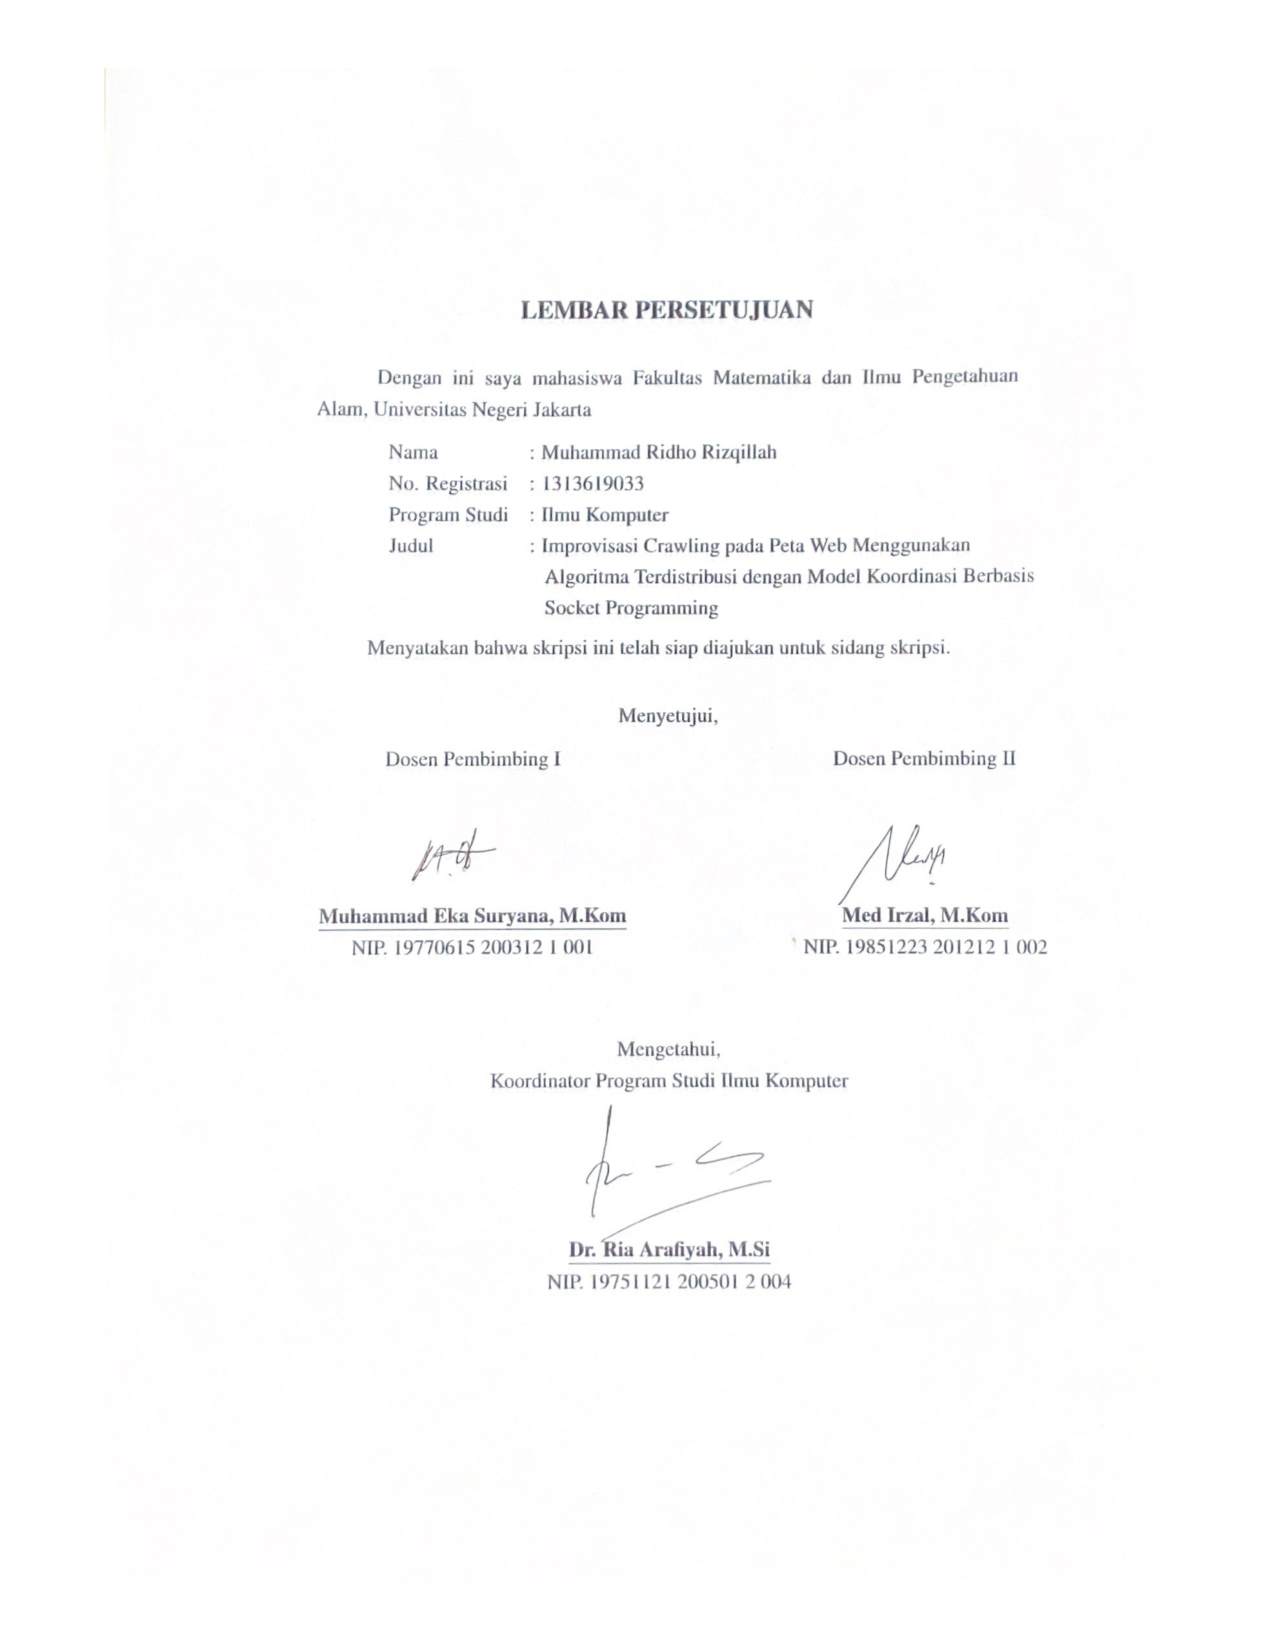
\includepdf[pages=-]{pdf/Lembar_Pengesahan_Skripsi.pdf}
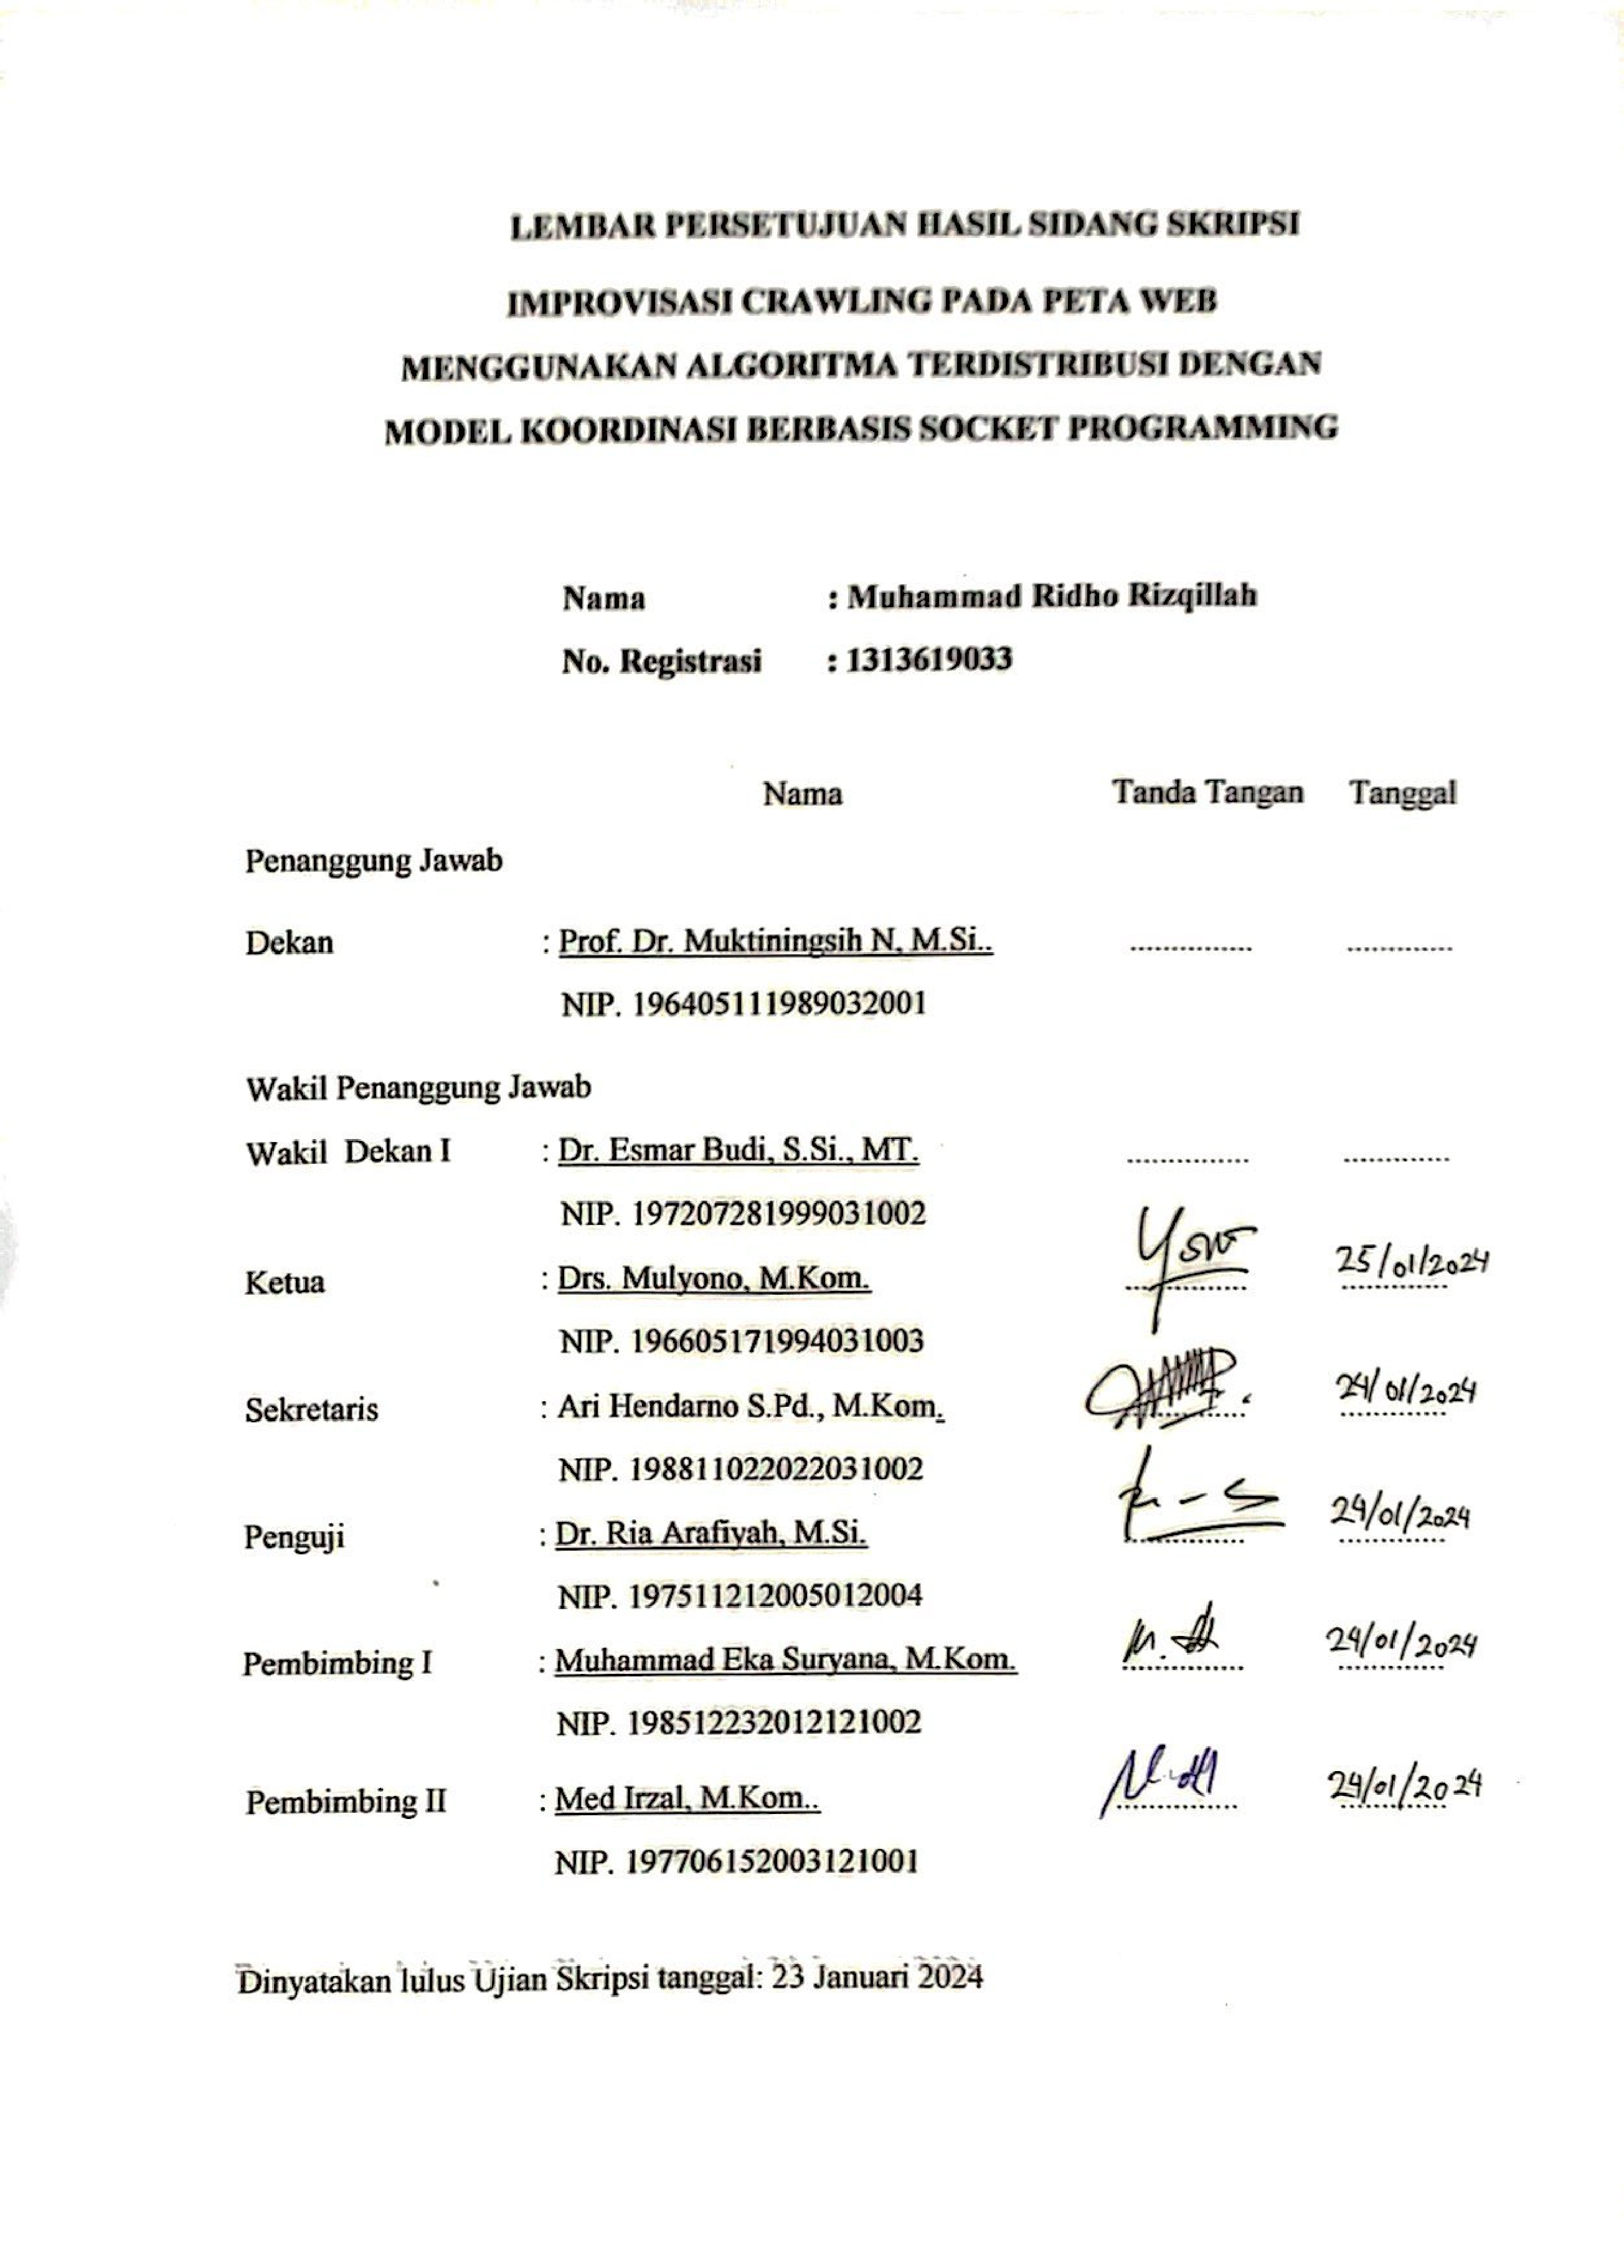
\includepdf[pages=-]{pdf/Lembar_Persetujuan_Revisi_Skripsi.pdf}
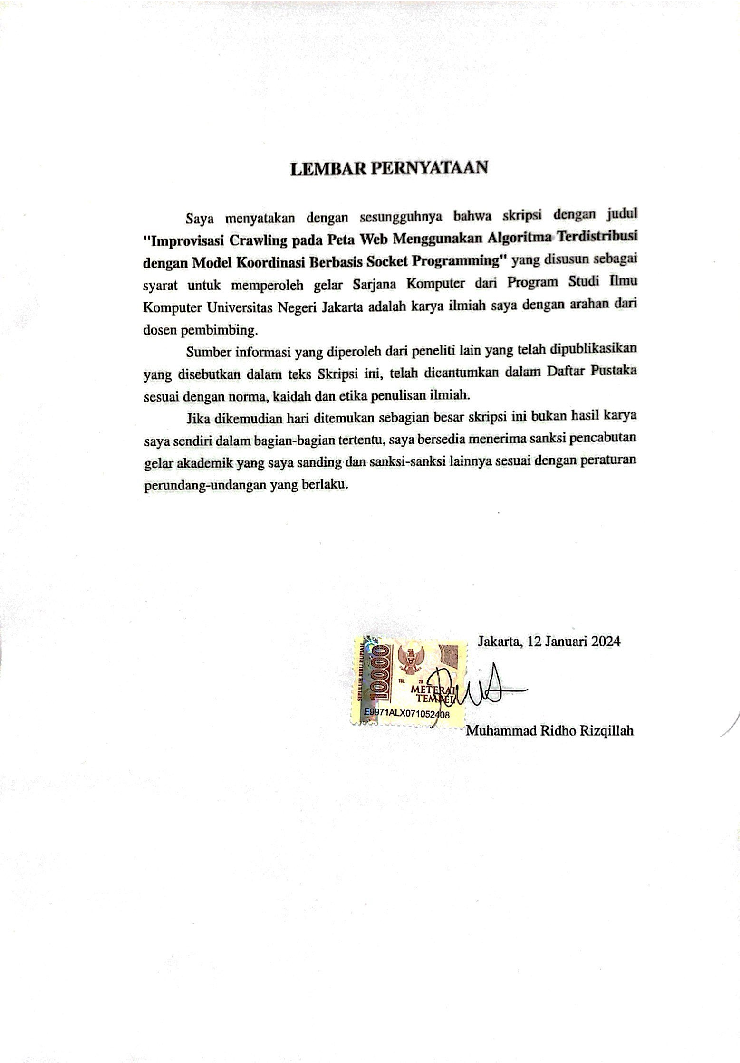
\includepdf[pages=-]{pdf/Lembar_Pernyataan.pdf}
\chapter*{\centering{\large{KATA PENGANTAR}}}
\onehalfspacing{}
Puji syukur penulis panjatkan ke hadirat Allah SWT, karena dengan rahmat dan
karunia-Nya, penulis dapat menyelesaikan skripsi yang berjudul
\textit{Improvisasi Crawling pada Peta Web Menggunakan Algoritma Terdistribusi dengan Model Koordinasi Berbasis Socket Programming}.

Keberhasilan penyusunan skripsi ini merupakan hasil dari kerja sama yang erat dengan berbagai pihak yang dengan tulus dan ikhlas memberikan kontribusi berharga untuk menyempurnakan penyusunan skripsi ini. Penulis merasa perlu menyampaikan rasa terima kasih dengan kerendahan hati kepada semua pihak yang telah turut serta memberikan bantuan dan masukan dalam proses penyusunan skripsi ini. Dalam kesempatan ini, penulis ingin mengekspresikan rasa syukur yang mendalam atas dukungan dan kerja sama yang telah diberikan oleh berbagai individu dan lembaga yang turut berperan dalam keberhasilan skripsi ini.

\begin{enumerate}

	\item{Yth. Para petinggi di lingkungan FMIPA Universitas Negeri Jakarta.}
	\item{Yth. Ibu Dr. Ria Arafiyah, M.Si selaku Koordinator Program Studi Ilmu
		Komputer.}
	\item{Yth. Bapak Muhammad Eka Suryana, M.Kom selaku Dosen Pembimbing I yang
		telah membimbing, mengarahkan, serta memberikan saran dan koreksi terhadap
	 skripsi ini.}
	\item{Yth. Bapak Med Irzal, M.Kom selaku Dosen Pembimbing II yang telah
		membimbing, mengarahkan, serta memberikan saran dan koreksi terhadap
	 skripsi ini.}
	\item{Kedua orang tua, kakak, dan adik penulis yang telah mendukung dan memberikan 
		semangat serta doa untuk penulis.}
	\item{Teman - teman Program Studi Ilmu Komputer 2019 yang telah memberikan 
		dukungan dan dorongan untuk menyelesaikan skripsi ini.}
	\item{Teman - teman Warteg yang bersedia memberikan dukungan dan kebersamaan dalam menyelesaikan skripsi ini.}
	\item{Salah satu adik tingkat yang serta merta menemani, mendengarkan keluh kesah, memberikan doa, dan semangat.}
	
\end{enumerate}

Penulis menyadari bahwa penyusunan skripsi ini masih jauh dari sempurna
karena keterbatasan ilmu dan pengalaman yang dimiliki. Oleh karenanya, kritik
dan saran yang bersifat membangun akan penulis terima dengan senang hati. Akhir
kata, penulis berharap tugas akhir ini bisa bermanfaat bagi semua pihak
khususnya penulis sendiri. Semoga Allah SWT senantiasa membalas kebaikan semua
pihak yang telah membantu penulis dalam menyelesaikan skripsi ini.

\vspace{4cm}

\begin{tabular}{p{7.5cm}c}
	&Jakarta, 12 Januari 2024\\
	&\\
	&\\
	&\\
	&Muhammad Ridho Rizqillah
\end{tabular}


%-----------------------------------------------------------------
%Disini awal masukan Intisari
%-----------------------------------------------------------------
\begin{abstractind}

	\textbf{Muhammad Ridho Rizqillah}. 	\textbf{Improvisasi \emph{Crawling} pada Peta Web Menggunakan
  Algoritma Terdistribusi dengan Model Koordinasi Berbasis
  \emph{Socket Programming}}. Skripsi. Program Studi Ilmu Komputer. Fakultas Matematika dan Ilmu Pengetahuan Alam, Universitas Negeri Jakarta. Januari 2024. Di bawah bimbingan Muhammad Eka Suryana, M. Kom. dan Med Irzal, M. Kom.
	\vskip5mm
	
	Mesin pencari memerlukan jumlah data yang besar untuk berjalan dengan optimal. Data yang besar diperlukan proses \emph{crawling} yang masif. Penelitian ini mencoba meningkatkan efisiensi \emph{crawling} dengan mengimplementasikan \emph{crawler} terdistribusi menggunakan \emph{socket} sebagai media komunikasi antar perangkat. Sistem arsitektur \emph{crawler} terdistribusi mencakup \emph{tracker}, \emph{manager}, dan \emph{client}. Tujuan utamanya adalah untuk meningkatkan efisiensi dan efektivitas \emph{crawling} dengan cara terdistribusi. Hasil akhir dari improvisasi ini menunjukkan peningkatan data sebanyak 30\% secara terdistribusi dengan dua \emph{crawler}, dibanding dengan \emph{crawler} individual. Serta tidak adanya data yang terduplikasi.
	
	\bigskip
	\noindent
	\textbf{Kata kunci :} \emph{search engine}, \emph{distributed crawler}, \emph{socket programming}, \emph{crawling}.
\end{abstractind}

\begin{abstracteng}
	
	\textbf{Muhammad Ridho Rizqillah}. 	\textbf{Improvisasi \emph{Crawling} pada Peta Web Menggunakan
  Algoritma Terdistribusi dengan Model Koordinasi Berbasis
  \emph{Socket Programming}}. Mini Thesis. Computer Science. Faculty of Mathematics and Natural Sciences, State University of Jakarta. January 2024. Under the guidance of Muhammad Eka Suryana, M. Kom. and Med Irzal, M. Kom.
	\vskip5mm
	
	Search engines require large amounts of data to run with optimal. Big data requires a massive crawling process. This research trying to improve crawling efficiency by implementing crawlers distributed using sockets as a communication medium between devices. System Distributed crawler architecture includes tracker, manager, and client. Objective The main thing is to increase the efficiency and effectiveness of crawling by means distributed. The final result of this improvisation shows an increase in data as much as 30\% distributed with two crawlers, compared to a crawler individual. And there is no duplicate data.
	
	\bigskip
	\noindent
	\textbf{Keyword :} search engine, distributed crawler, socket programming, crawling.
\end{abstracteng}


%-----------------------------------------------------------------
%Disini akhir masukan Intisari
%-----------------------------------------------------------------
%-----------------------------------------------------------------


\singlespacing{}
\tableofcontents{}
\addcontentsline{toc}{chapter}{DAFTAR ISI}
\listoffigures{}
\addcontentsline{toc}{chapter}{DAFTAR GAMBAR}
\listoftables{}
\addcontentsline{toc}{chapter}{DAFTAR TABEL}

\begin{counterpage}
\end{counterpage}
%Disini awal masukan untuk Bab
%-----------------------------------------------------------------
\onehalfspacing{}
%!TEX root = ./template-skripsi.tex
%-------------------------------------------------------------------------------
% 								BAB I
% 							LATAR BELAKANG
%-------------------------------------------------------------------------------

\chapter{PENDAHULUAN}

\section{Latar Belakang Masalah}

Mesin pencari atau \emph{search engine} adalah sebuah teknologi yang digunakan untuk mencari sebuah informasi yang tersedia di internet. Dengan memasukkan \emph{keyword} terkait hal yang ingin diketahui dan akan terlihat berbagai macam situs \emph{web} yang memiliki informasi sesuai. Perkembangan \emph{search engine} melahirkan penelitian yang berkelanjutan, meneliti bagaimana menciptakan algoritma yang efektif untuk menjalankan \emph{search engine} agar menampilkan pencarian yang relevan kepada pengguna.  

Penelitian \emph{search engine} yang dilakukan sebelumnya lebih terfokus untuk mengembangkan \emph{crawler} yang dapat berjalan secara \emph{multi-threaded} (\cite{fathan2021search}). Sedangkan pada penelitian selanjutnya mengarah pada \emph{refactoring crawler} dari penelitian sebelumnya dan mencari \emph{similarity score} dari setiap halaman situs \emph{web} yang di-\emph{crawling} (\cite{lazuardy2023search}). Dan penelitian lainnya saat melakukan pengumpulan data menggunakan \emph{crawler} yang sudah ada agar dapat dikelola dalam bentuk \emph{user interface} (\cite{aldian2024search}).

Kelemahan yang terdapat pada penelitian tersebut adalah \emph{crawling} hanya dapat berjalan pada satu perangkat saja. Hal itu dapat menghambat hasil dari \emph{crawling}, karena membutuhkan waktu lebih lama untuk mendapatkan hasil \emph{crawling} yang masif. Oleh karena itu, diperlukan cara agar \emph{crawler} dapat berjalan pada berbagai macam perangkat atau terdistribusi satu dengan lainnya. Serta kelemahan yang didapatkan bahwa proses \emph{crawling} dengan \emph{public IP address} dapat menyebabkan \emph{IP public} perangkat terblokir oleh Cloudflare atau layanan penyedia internet, sebab dianggap perilaku mencurigakan.

Terdapat juga kelemahan lainnya pada \emph{database}. \emph{Wasting storage} yang cukup besar terhadap kolom - kolom yang tidak terlalu diperlukan untuk \emph{similarity scoring}. Maka, peneliti melakukan analisis terkait \emph{database}-nya dengan melakukan \emph{crawling} selama 48 jam, didapatkan hasil laporan \emph{database} pada gambar 1.1. Total dari keseluruhan \emph{database}-nya adalah 8.7 GB.

\begin{figure}[H]
	\centering
	
\includegraphics[width=1\textwidth]{gambar/db_analisis}
	\caption{\emph{Analisis Database Penelitian Crawling}}
	\label{gambar:db_analisis}
\end{figure}

Terdapat \emph{wasting storage} pada \emph{table page\_list}, mengandung kumpulan \emph{tag} <li>. \emph{page\_scripts}, mengandung skrip \emph{javasript}. \emph{page\_styles}, mengandung \emph{style} dari CSS (\emph{Cascading Style Sheet}). \emph{page\_tables}, mengandung \emph{tag <table>}. Karena memiliki ukuran yang besar dan informasi yang didapatkan kurang berguna untuk melakukan \emph{page ranking}. Bahkan ukuran dari \emph{tables} yang disebutkan di atas dapat memenuhi setidaknya lebih dari 60\% dari total ukuran \emph{database}.

Sedangkan \emph{tables} yang berguna untuk hasil dari \emph{crawling} adalah: \emph{Table crawling}, untuk menjelaskan \emph{starting url}, \emph{total page}, durasi \emph{crawl}, dan tanggal \emph{crawling} berakhir. Lalu, pada \emph{table page\_linking} untuk mengetahui \emph{outgoing link}, yang nantinya akan digunakan untuk \emph{page ranking}. Pada \emph{table page\_information} diperlukan untuk mendapatkan \emph{initial page rank}, yang hasilnya didapatkan dari 1 / total baris \emph{table page\_information}. Dan juga berguna untuk \emph{document ranking tf-idf} dengan mengambil setiap kata yang ada. Melalui hasil analisis \emph{database} berikut, bahwa data penting yang digunakan untuk \emph{page rank} dan \emph{tf idf} adalah pada \emph{table crawling, page\_information, dan page\_linking}.

Diperlukan improvisasi pada algoritma dan menambahkan cara untuk membagi tugas \emph{crawling} supaya menjadi versi terdistribusi. \emph{Crawling} terdistribusi adalah melakukan \emph{crawling} secara terpisah ke setiap perangkat yang tersedia, guna membagi beban kerja dan dapat menghasilkan hasil \emph{crawler} dalam jumlah yang masif secara efisien serta efektif. Sebelum melakukan improvisasi \emph{crawler} yang sekarang menjadi terdistribusi, diperlukan pemahaman terkait sistem arsitekturnya.

Sistem arsitektur \emph{crawler} terdistribusi memiliki dua komponen penting, yaitu \emph{crawling system} dan \emph{crawling application}. \emph{Crawling System} meliputi \emph{crawl manager}, \emph{downloader}, dan \emph{DNS resolvers}. Sedangkan \emph{crawling application} yang melakukan proses \emph{crawling} yang berjalan pada perangkat.

% \begin{figure}[H]
% 	\centering
% 	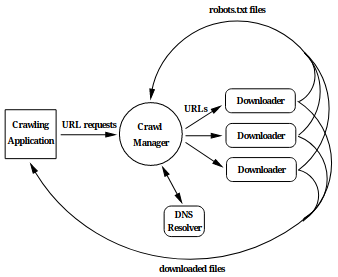
\includegraphics[width=0.5\textwidth]{gambar/arsitektur_terdistribusi}
% 	\caption{\emph{Arsitektur Sederhana Crawler Terdistribusi}}
% 	\label{gambar:arsitektur_terdistribusi}
% \end{figure}

Berdasarkan arsitektur sederhana didapatkan bahwa proses distribusi yang terjadi adalah pada sisi \emph{downloader}. Setelah \emph{crawl manager} melakukan \emph{crawling} pada suatu \emph{web} yang akan menghasilkan \emph{urls}, kemudian \emph{url} tersebut dilanjutkan kepada masing - masing \emph{downloader}. \emph{Downloader} ini terletak pada \emph{server} atau perangkat yang berbeda (\cite{shkapenyuk2002distributed}).

Komunikasi yang dilakukan dalam arsitektur tersebut dilakukan dalam dua cara yaitu, via \emph{socket} dan \emph{file system} untuk data yang lebih besar. Untuk improvisasi yang akan diterapkan dalam proyek ini akan lebih tertuju kepada penerapan \emph{socket}.

\emph{Socket} dapat dianggap sebagai \emph{endpoint} dalam \emph{two-way communication channel}. \emph{Socket} dapat melakukan komunikasi antara dua proses, baik dalam satu perangkat atau perangkat yang berbeda. Untuk dapat melakukan komunikasi dua arah, terlebih dahulu dipahami arsitektur \emph{client-server}. \emph{Client} dapat berupa PC, laptop, telepon seluler, dll. Dan setiap \emph{client} memiliki IP \emph{address}-nya masing - masing. Untuk dapat melakukan komunikasi atau pertukaran data diperlukan setiap \emph{client} untuk terhubung ke sebuah \emph{server}. \emph{Server} pun juga memiliki IP \emph{address}. Agar \emph{client} dapat terhubung ke \emph{server}, maka ia harus mengetahui IP \emph{server}. Dan setiap \emph{client} yang terhubung ke \emph{server} akan dapat berkomunikasi via \emph{server} dalam hal ini akan menggunakan \emph{socket} (\cite{ibm2021whatissocket}).

% Penggunaan SOCK\_STREAM berarti memakai \emph{protocol} TCP. Kalau ingin memakai \emph{protocol} UDP, maka menggunakan SOCK\_DGRAM. Di sini saya menggunakan TCP karena beberapa keunggulan seperti, \emph{reliable} (dapat mendeteksi \emph{packet loss}), dapat memastikan data terkirim, \emph{sequential} (data yang dikirim berurutan), \emph{byte stream} (data yang dikirim dalam bentuk \emph{byte}, lebih efisien), \emph{keeps up connection}. Kalau dibandingkan dengan UDP seperti, \emph{sends one datagram, no order and guarantee, more realtime} (karena tidak memperdulikan \emph{packet loss}, jadi lebih cepat), \emph{less network} and \emph{pc stress} \cite{neuralnine2021socket}.

% \begin{figure}[H]
% 	\centering
% 	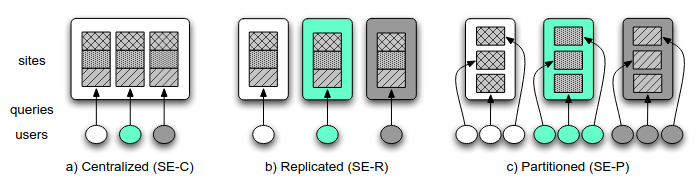
\includegraphics[width=0.85\textwidth]{gambar/arsitektur_query_processing}
% 	\caption{\emph{Arsitektur Sederhana Crawler Terdistribusi}}
% 	\label{gambar:arsitektur_query_processing}
% \end{figure}

Pada penelitian lain terkait \emph{query processing} dan alokasi komputasional \emph{crawler} terdistribusi yang dilakukan oleh Cambazoglu terdapat beberapa jenis arsitektur berdasarkan cara penyimpanan \emph{index}-nya. Secara \emph{centralized} (SE-C), \emph{replicated} (SE-R), dan \emph{partitioned} (SE-P). Ada juga arsitektur gabungan antara \emph{partial replication} dan \emph{query forwarding} (SE-H). Arsitektur \emph{centralized} masih banyak digunakan sampai sekarang, apalagi dalam skala yang lebih kecil (\cite{cambazoglu2009quantifying}).

% \begin{figure}[H]
% 	\centering
% 	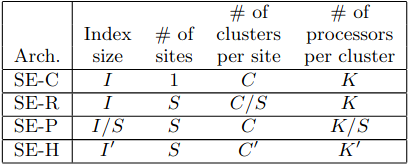
\includegraphics[width=0.5\textwidth]{gambar/resource_allocation_on_search_engine}
% 	\caption{\emph{Alokasi Sumber Daya pada Berbagai Arsitektur Search Engine}}
% 	\label{gambar:resource_allocation_on_search_engine}
% \end{figure}

% Pada pemrosesan query ada dua tipe cost, fixed cost independent dari jumlah processor dan cost linear dengan pertambahan jumlah processor. Rata - rata waktu yang diperlukan untuk memproses query (T) dapat direpresentasikan dalam persamaan 

% \begin{equation*}
%   T = a + b × Iavg/K,
% \end{equation*}
% a adalah fixed time cost, b adalah time cost untuk memproses byte pada inverted list, Iavg adalah rata - rata ukuran index. dan K adalah jumlah processor di tiap klaster \cite{cambazoglu2009quantifying}.

% \begin{figure}[H]
% 	\centering
% 	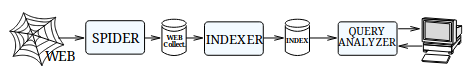
\includegraphics[width=0.85\textwidth]{gambar/typical_web_search_engine_architecture}
% 	\caption{\emph{Tipikal Arsitektur Web Search Engine}}
% 	\label{gambar:typical_web_search_engine_architecture}
% \end{figure}

Pada penelitian yang dilakukan oleh (\cite{orlando2002design}) menjelaskan bahwa dalam \emph{web search engine} terdiri dari \emph{spidering system}. Kesatuan dari sistem ini berjalan secara paralel, yang mana \emph{crawler} akan mengunjungi setiap \emph{web} dan mengumpulkan informasi yang diperlukan. Inti utama dalam \emph{Information Retrieval} (IR) adalah \emph{indexer} dan \emph{query analyzer}. 

% Hasil dari informasi yang didapatkan akan di-\emph{ranking} berdasarkan kesesuaiannya dengan \emph{query} yang dimasukkan, untuk mendapatkan hasil akhir yang sesuai dan efisien, banyak arsitektur search engine sekarang menerapkan Inverted List untuk indexing. Ada dua komponen penting dari Inverted List yaitu Lexicon dan Postings list.

Pada tahapan \emph{query analyzer} melakukan proses paralel terhadap \emph{Query Brokers} dan \emph{Local Searchers}. Dilakukan secara terdistribusi menggunakan teknik \emph{document partitioning}. Strategi untuk membuat paralel \emph{web search engine} harus memenuhi dua hal, \emph{task parallel} dan \emph{data parallel}. Untuk menghindari eksploitasi \emph{processor} secara berlebihan, maka diperlukan \emph{load balancer}, agar setiap \emph{query} dapat berjalan secara efisien dan efektif. Dengan melakukan pembagian \emph{task} secara paralel. Oleh karena setiap \emph{query} diproses secara terpisah, maka juga memiliki partisi \emph{database}-nya tersendiri. Untuk itu diperlukan kombinasi antara \emph{task} dan \emph{data parallel}, agar hasil akhir dari proses \emph{search engine} lebih relevan (\cite{orlando2002design}).

Pada penelitian lain dijelaskan juga mengenai distribusi algoritma, walaupun diterapkan pada perhitungan \emph{page rank} agar lebih efisien memori dalam melakukan perhitungan. Karena untuk perhitungannya diperlukan memori yang besar. Oleh karena itu, diperlukan proses efisiensi memori (\cite{farhan2023page}). Walaupun begitu data perhitungan akan berkurang karena efisiensi memori, memang ada hal yang menjadi timbal baliknya. Nanti hasil dari penelitian tersebut juga akan diterapkan untuk penelitian lebih lanjut setelah penelitian yang penulis lakukan.

Berdasarkan beberapa rujukan sebelumnya, hasil dari penelitian ini adalah sebuah \emph{crawler} yang berjalan secara terdistribusi yang akan mengimplementasikan penggunaan \emph{socket} dalam mendistribusikan tugas ke setiap perangkat, serta peningkatan jumlah data yang terkumpul.

% Menerapkan \emph{time cost efficiency} dalam melakukan \emph{query processing}, serta melakukan \emph{task parallel} yang baik dengan keseimbangan tugas. Untuk arsitekturnya akan merujuk arsitektur gabungan antara \emph{partial replication} dan \emph{query forwarding} (SE-H).

\section{Rumusan Masalah}
Berdasarkan uraian pada latar belakang yang diutarakan di atas, maka perumusan masalah pada penelitian ini adalah "\textbf{bagaimana meningkatkan efisien \emph{crawling} dengan cara terdistribusi?}".

\section{Pembatasan Masalah}
Pembatasan masalah pada penelitian ini antara lain:
\begin{enumerate}
	\item Pengembangan arsitektur \emph{crawler} menjadi versi terdistribusi dengan skala kinerja 2 hingga 5 perangkat.
	\item \emph{Crawler} terdistribusi yang dikembangkan menggunakan \emph{socket} sebagai media komunikasi antar perangkat.
	\item Pengujian terhadap \emph{crawler} terdistribusi dan tidak terdistribusi yang akan mempertimbangkan faktor-faktor seperti kecepatan crawling dan efisiensi penggunaan sumber daya.
\end{enumerate}

\section{Tujuan Penelitian}
Tujuan penelitian pada penelitian ini antara lain:
\begin{enumerate}
	\item Mengembangkan arsitektur \emph{distributed crawler}.
	\item Membuat implementasi \emph{socket} untuk memenuhi kebutuhan improvisasi \emph{crawler}.
\end{enumerate}

\section{Manfaat Penelitian}
\begin{enumerate}
	\item Bagi penulis
		
	Menambah pengetahuan di bidang sistem terdistribusi mengenai \emph{search engine} dan \emph{crawling}, mengasah kemampuan programming, dan memperoleh gelar sarjana di bidang Ilmu Komputer. Selain itu, penulisan ini juga merupakan media bagi penulis untuk mengaplikasikan ilmu yang didapat di kampus ke kehidupan masyarakat.
		
	\item Bagi Universitas Negeri Jakarta 
	 	
	Menjadi pertimbangan dan evaluasi akademik khususnya Program Studi Ilmu Komputer dalam penyusunan skripsi sehingga dapat meningkatkan kualitas akademik di program studi Ilmu Komputer Universitas Negeri Jakarta serta meningkatkan kualitas lulusannya.
	 			
\end{enumerate}


% Baris ini digunakan untuk membantu dalam melakukan sitasi
% Karena diapit dengan comment, maka baris ini akan diabaikan
% oleh compiler LaTeX.
\begin{comment}
\bibliography{daftar-pustaka}
\end{comment}

%!TEX root = ./template-skripsi.tex
%-------------------------------------------------------------------------------
%                            BAB II
%               KAJIAN TEORI
%-------------------------------------------------------------------------------

\chapter{KAJIAN PUSTAKA}

\section{Jaringan Komputer}

Jaringan komputer adalah sekumpulan perangkat komputasi yang saling terhubung satu sama lain. Seperti dua komputer yang saling terhubung dan dapat bertukar informasi. Interkoneksi dapat berlangsung pada berbagai macam media transmisi, seperti kawat tembaga, kabel \emph{fiber optic}, dan gelombang radio. Internet adalah contoh yang sering dijumpai sebagai jaringan dari banyak jaringan.

Peran jaringan komputer yang sangat umum adalah untuk mendapatkan akses terhadap suatu informasi. Cara pengaksesan informasi ini pun dapat melalui berbagai cara, menggunakan internet dengan \emph{web browser}, mengakses informasi melalui media sosial. Bahkan dengan menggunakan \emph{smartphone} sudah dapat mengakses banyak informasi dengan internet yang terhubung. Banyak informasi yang diakses melalui internet menggunakan model \emph{client-server}, klien meminta informasi kepada server melalui jaringan, dan server mengembalikan informasi yang dibutuhkan oleh klien. Model ini sudah banyak dan secara luas diterapkan dalam proses mendapatkan informasi. Model lain yang cukup populer adalah \emph{peer-to-peer}, dalam proses komunikasi \emph{peer-to-peer} dapat langsung berhubungan dengan klien atau server dan tidak pasti siapa yang akan menjadi klien atau server. Jadi, keduanya dapat bertukar informasi secara langsung.

\section{Protokol Jaringan}

Protokol jaringan adalah aturan yang ada pada jaringan. Kegunaannya untuk menjaga agar jaringan yang digunakan dapat berjalan dengan baik. Beberapa hal yang perlu diperhatikan pada protokol jaringan yaitu:

\begin{enumerate}
  \item{\emph{Reliability}}

  Agar suatu jaringan dapat beroperasi dengan normal, perlu adanya \emph{reliability} atau keandalan. Sebab, sering dijumpai beberapa kesalahan dalam transmisi informasi, seperti \emph{electrical noise}, \emph{random wireless signal}, dll. Cara mengatasinya hal tersebut terjadi dengan menerapkan \emph{error detection}. Dengan demikian lebih mudah untuk mengetahui kemungkinan \emph{error} yang terjadi dan dapat diperbaiki dengan cepat. Alangkah baiknya jika diterapkan juga \emph{error correction}. Ketika terjadi \emph{error}, maka dengan otomatis akan teratasi. Sebagai contoh ketika terdapat gangguan koneksi di suatu rute transmisi, maka akan teratasi dengan mengubah jalur transmisi ke rute yang lain.

  \item{\emph{Resource Allocation}}

  Semakin besar dan berkembang suatu jaringan, akan timbul permasalahan baru. Seperti \emph{resource} atau sumber data yang semakin terbatas. Ketika ingin meminta informasi, dari klien kepada server, karena semakin besar jaringan yang ada dalam suatu lingkup. Maka akan terjadi \emph{traffic} yang tinggi sebab banyaknya klien yang meminta informasi dalam waktu yang bersamaan. Untuk mengatasi hal ini, diperlukan pembatasan terhadap permintaan atau menerapkan \emph{bandwidth}. Dengan adanya \emph{bandwidth}, setiap klien memiliki batasan untuk meminta sebuah informasi pada waktu yang ditentukan.

  \item{\emph{Evolvability}}

  Berkembangnya jaringan dari waktu ke waktu memerlukan adaptasi terhadap jaringan yang ada sebelumnya. Perubahan struktur jaringan dan mekanisme yang digunakan perlu diselaraskan dengan jaringan yang terdahulu sudah ada. Karena tidak mungkin perubahan dilakukan secara drastis dan menghapus total jaringan terdahulu. Perlu ada masa peralihan dan penyesuaian.

  \item{\emph{Security}}
  
  Keamanan adalah faktor penting dalam jaringan. Untuk menghadapi berbagai macam ancaman yang ada diperlukan keamanan yang memadai. Salah satu mekanisme yang diterapkan adalah dengan menggunakan autentikasi, dengan adanya autentikasi menjadikan seseorang menjadi lebih jelas identitasnya dan tidak akan mudah untuk melakukan penyamaran.
\end{enumerate}

\section{Protocol Layering}

Untuk mengurangi kompleksitas dalam jaringan, dibentuk sebuah \emph{layer} atau lapisan. Masing - masing lapisan terbentuk berdasar lapisan yang ada di bawahnya. Dengan pembuatan lapisan ini menyediakan layanan dan kebutuhan untuk lapisan berikutnya yang lebih tinggi, sementara melindungi detail penting dari setiap lapisan dan implementasinya. Hal ini mirip seperti konsep pada \emph{Object Oriented Programming} (OOP) yang mana terdapat pilar - pilar yang terdiri dari \emph{abstraction} dan \emph{encapsulation}. Berguna untuk hanya menampilkan info yang penting dari setiap lapisan dan menjaga agar setiap lapisan memiliki fungsinya masing - masing.

\begin{figure}[H]
  \centering{}
	\includegraphics[width=0.85\textwidth]{gambar/protocol\_layering}
  \caption{Five-Layer Network}
\end{figure}

Pada Gambar 2.1 adalah contoh dari \emph{five-layer network}. Entitas yang terdiri dari setiap lapisan itu disebut dengan \emph{peers}. \emph{Peers} dapat berupa proses perangkat lunak, perangkat keras, atau bahkan manusia. Setiap \emph{peers} berkomunikasi menggunakan protokol. Proses transmisi data yang terjadi tidak serta merta langsung antara satu lapisan pada satu perangkat menuju lapisan yang sama pada perangkat yang lain. Melainkan prosesnya terjadi dari lapisan paling atas menuju ke lapisan paling bawah sampai mencapai physical medium, setelah itu baru komunikasi berlanjut pada lapisan itu. Garis putus - putus menunjukkan \emph{virtual communication} melalui protokol dan garis tidak putus - putus menunjukkan \emph{physical communication} antara tiap lapisan.

Diantara setiap lapisan terdapat \emph{interface}. \emph{Interface} bertujuan untuk mendefinisikan operasi dan layanan apa saja yang disediakan lapisan bawah untuk lapisan atasnya. Hal penting yang harus diperhatikan dalam mendesain jaringan adalah clean \emph{interface} agar menjadi lebih jelas apa fungsi dari setiap lapisannya.

Berbagai lapisan menawarkan dua opsi layanan koneksi: \emph{connection-oriented} dan \emph{connectionless}. Pada \emph{connection-oriented}, seperti halnya koneksi telepon. Untuk menggunakan telepon, pemanggil memasukan nomor tujuan dan menelponnya. Pada pihak penerima mendapatkan panggilan dan mengangkat telepon, barulah koneksi terhubung dan terjadi. pemanggil memberikan sebuah informasi dan diterima oleh penerima dan begitupun sebaliknya. Pada \emph{connectionless}, seperti halnya surat fisik pada layanan pos. Pengirim mengirim surat kepada penerima dengan alamatnya. Pesan tersebut akan diterima dalam kurun beberapa hari, bisa sampai dengan tepat waktu atau lebih lambat. Jika penerima juga mengirim surat yang berbeda kepada pengirim pada waktu berikutnya, bisa saja surat dari penerima yang sampai duluan. Tidak semua aplikasi membutuhkan koneksi antara dua belah pihak. Seperti halnya seorang penipu bisa saja mengirimkan satu email kepada banyak penerima. Tanpa peduli pesan tersebut dibaca oleh penerima. Layanan \emph{connectionless} biasa disebut sebagai \emph{datagram service}.

Kedua layanan tersebut dapat dikategorikan berdasarkan \emph{reliability}. Penggunaan \emph{connection-oriented} menjamin pengirim mengirimkan data kepada penerima, data yang dikirimkan dapat diterima secara lengkap, tidak ada kekurangan dan dapat menghindari duplikasi data. Terkadang memiliki \emph{cost} yang besar untuk mengimplementasikan layanan ini. Sedangkan \emph{connectionless} tidak memerlukan koneksi yang stabil antara pengirim dan penerima. Pengiriman data yang dilakukan berjalan secara lebih sederhana. Pengirim hanya perlu mengirim data, tidak memperdulikan data yang tidak sampai dengan jelas, duplikasi, dan tidak berurutan. Penggunaan \emph{connectionless} lebih menguntungkan ketika terjadi \emph{online meeting}, karena video yang tetap dapat terlihat dan diterima walaupun ada beberapa \emph{pixels} yang salah. Dibandingkan jika harus menunggu keseluruhan video terlihat jelas menggunakan \emph{connection-oriented}, tapi perlu menunggu lebih lama untuk menampilkannya.


\section{\emph{TCP/IP Model}}

TCP/IP Model banyak digunakan oleh jaringan komputer secara menyeluruh dari internet di seluruh dunia. Ketika satelit dan jaringan radio hadir, protokol yang ada memiliki masalah dalam beroperasi dengannya, jadi diperlukan model arsitektur yang baru. Oleh karena itu, kemampuan TCP/IP dari awal adalah untuk dapat menghubungkan beberapa jaringan dengan lancar yang merupakan salah satu tujuan utama dari model ini. Arsitektur ini kemudian dikenal sebagai \emph{TCP/IP Reference Model}.

\begin{figure}[H]
  \centering{}
	\includegraphics[width=0.85\textwidth]{gambar/osi\_tcp\_ip\_model}
  \caption{OSI dan TCP/IP Model}
\end{figure}

Pada Gambar 2.2 terdapat dua model, yaitu OSI dan TCP/IP. OSI (\emph{Open Systems Interconnection}) dinamakan seperti itu karena berkaitan dengan menghubungkan \emph{open system} atau sistem terbuka untuk berkomunikasi dengan sistem lainnya. Pada OSI model terdiri dari tujuh lapisan dan setiap lapisannya memiliki beberapa layanan untuk lapisan di atasnya. OSI model memiliki tiga konsep penting: \emph{services}, \emph{interfaces}, dan \emph{protocols}. Perbedaan dari OSI dan TCP/IP adalah perubahan pada lapisannya, TCP/IP tidak memiliki lapisan physical, session, dan presentation. TCP/IP merupakan pembaruan dari OSI model. Terdapat empat lapisan pada TCP/IP dan contoh protokolnya pada Gambar 2.3.

\begin{figure}[H]
  \centering{}
	\includegraphics[width=0.85\textwidth]{gambar/tcp\_ip\_model}
  \caption{TCP/IP Model dan Protokolnya}
\end{figure}

\subsection{\emph{Link Layer}}

Sebagai lapisan paling bawah dalam model TCP/IP lapisan \emph{link} sering dibandingkan dengan kombinasi dari lapisan data \emph{link} dan \emph{physical}. Fungsi dari lapisan ini adalah untuk menyediakan layanan kepada lapisan jaringan atau internet agar dapat mentransfer data dari lapisan jaringan yang berada pada \emph{source machine} menuju \emph{destination machine}. Dan menghubungkan antara \emph{physical} dan \emph{logical network}.

% \subsubsection{\emph{Design Issues}}

% Terdapat beberapa hal penting pada lapisan ini yang perlu diperhatikan, yaitu: menyediakan layanan yang tepat untuk lapisan di atasnya, konsep \emph{framing bytes}, mendeteksi dan memperbaiki transmisi yang bermasalah, dan meregulasi aliran data. Lapisan \emph{link} dapat dirancang untuk menawarkan berbagai layanan. Layanan sebenarnya yang ditawarkan bervariasi dari satu protokol ke protokol lainnya. Terdapat tiga jenis layanan yaitu:

% \begin{enumerate}
%   \item{\emph{Unacknowledged connectionless service}}

%   \emph{Unacknowledged connectionless service} memiliki \emph{source machine}, mengirim \emph{frame} independen ke \emph{destination machine} tanpa diketahui olehnya. Ethernet adalah contoh yang baik dari lapisan \emph{link}. Tidak ada \emph{logical connection} yang dikonfigurasi sebelumnya, atau dirilis sesudahnya. Tidak ada upaya yang dapat dilakukan dalam mendeteksi kerugian atau memulihkannya di lapisan \emph{link}, jika \emph{frame} hilang karena gangguan pada saluran. Layanan ini tepat digunakan untuk tingkat kesalahan yang sangat rendah, meninggalkan pemulihan ke lapisan yang lebih tinggi. Jadi pemulihan diserahkan ke lapisan yang lebih tinggi. Sesuai untuk lalu lintas \emph{real-time}, seperti suara atau video, di mana data yang datang terlambat lebih buruk dari data yang buruk.

%   \item{\emph{Acknowledged connectionless service}}

%   Ketika layanan ini digunakan, tetap tidak memerlukan \emph{logical connection}, tetapi setiap \emph{frame} yang dikirim diakui secara individual. Dengan cara ini, pengirim mengetahui apakah \emph{frame} telah tiba dengan benar atau hilang. Jika belum tiba dalam waktu yang ditentukan interval waktu, itu dapat dikirim lagi. Layanan ini berguna melalui saluran yang \emph{unreliable}, seperti sistem nirkabel. 802.11 (WiFi) adalah contoh yang baik dari jenis lapisan \emph{link} ini. Mungkin perlu ditekankan bahwa memberikan \emph{acknowledged} atau pengakuan dalam lapisan \emph{link} hanyalah pengoptimalan. Itu tidak pernah menjadi persyaratan.

%   \item{\emph{Acknowledged connection-oriented service}}

%   \emph{Acknowledged connection-oriented service} adalah layanan paling canggih dari lapisan \emph{link}. \emph{Source machine} dan \emph{destination} membuat koneksi sebelum ada data ditransfer. Setiap \emph{frame} yang dikirim melalui koneksi diberi nomor, dan lapisan \emph{link} menjamin bahwa setiap \emph{frame} yang dikirim benar-benar diterima. Ketika layanan ini digunakan, proses transfer melalui tiga fase. Pertama, koneksi dibuat dengan meminta kedua belah pihak menginisialisasi variabel dan \emph{counters} yang diperlukan untuk melacak \emph{frame} mana yang telah diterima dan mana yang belum. Kedua, satu atau lebih \emph{frame} ditransmisikan. Ketiga, koneksi dilepaskan, membebaskan variabel, \emph{buffer}, dan sumber daya lain yang digunakan untuk menjaga koneksi.
% \end{enumerate}

% Untuk menyediakan layanan ke lapisan jaringan, lapisan \emph{link} harus menggunakan layanan yang disediakan oleh lapisan \emph{physical}. Lapisan \emph{physical} menerima aliran \emph{raw bit} dan mencoba mengirimkannya ke tujuan. Jika saluran \emph{noisy}, seperti kebanyakan nirkabel dan beberapa tautan kabel, lapisan \emph{physical} akan menambahkan beberapa redundansi ke dalam sinyal untuk mengurangi tingkat kesalahan \emph{bit} ke tingkat yang dapat ditoleransi. Namun, aliran \emph{bit} yang kembali diterima oleh lapisan \emph{link} tidak dijamin bebas dari kesalahan. Beberapa \emph{bit} mungkin memiliki nilai yang berbeda, dan jumlah \emph{bit} yang diterima mungkin kurang dari, sama dengan, atau lebih dari jumlah \emph{bit} yang ditransmisikan. Pendekatan yang biasa dilakukan adalah lapisan \emph{link} untuk memecah aliran \emph{bit} menjadi \emph{frame} diskrit, menghitung \emph{token} pendek yang disebut \emph{checksum} untuk setiap \emph{frame}, dan menyertakan \emph{checksum} dalam \emph{frame} saat ditransmisikan. Terdapat empat metode untuk melakukan ini yaitu: \emph{byte count}, \emph{flag bytes with byte stuffing}, \emph{flag bits with bit stuffing}, dan \emph{physical layer coding violations}.

% Protokol \emph{link} dapat memberikan kontrol kesalahan untuk mendeteksi atau memperbaiki kerusakan \emph{frame} dan mentransmisikan ulang \emph{frame} yang hilang. Untuk mencegah pengirim cepat dari \emph{overrunning slow receiver}, protokol \emph{link} juga dapat menyediakan \emph{flow control}. Mekanisme \emph{sliding window} banyak digunakan untuk mengintegrasikan kontrol kesalahan dan kontrol aliran dengan cara sederhana. Ketika ukuran jendela adalah 1 paket, protokolnya adalah \emph{stop-and-wait}. 

% Kode untuk \emph{error correction} dan \emph{error detection} menambahkan informasi berlebihan ke pesan dengan menggunakan berbagai teknik matematika. Kode konvolusi dan kode \emph{Reed-Solomon} digunakan secara luas untuk koreksi kesalahan, dengan \emph{low-density parity check} semakin populer. Kode untuk deteksi kesalahan yaitu digunakan dalam praktik termasuk cek \emph{cyclic redundancy} dan \emph{checksum}. Semua kode ini dapat diterapkan pada lapisan \emph{link}, serta pada lapisan \emph{physical} dan lapisan yang lebih tinggi.

Pada lapisan ini terdapat tiga protokol sederhana saat melakukan transmisi data, yaitu:

\begin{enumerate}
  \item{\emph{Utopia: No Flow Control or Error Detection}}

  Pada protokol ini dibuat sederhana, dengan anggapan bahwa tidak ada kemungkinan terjadinya kesalahan. Data hanya ditransmisikan satu arah saja. Lapisan jaringan selalu siap untuk mentransmisikan dan menerima. Waktu pemrosesan dapat diabaikan. Ruang \emph{buffer} yang tak terbatas. Dan saluran komunikasi antara lapisan \emph{link} tidak pernah rusak atau kehilangan \emph{frame}. Oleh karena itu disebut sebagai `Utopia'. Protokol terdiri dari dua prosedur yang berbeda, pengirim dan penerima. Itu pengirim berjalan di lapisan \emph{link} dari \emph{source machine}, dan penerima berjalan masuk lapisan \emph{link} dari \emph{destination machine}. Tidak ada \emph{sequence numbers} atau \emph{acknowledgements} yang digunakan. Pengirim berada dalam \emph{while loop} yang tak terbatas yang hanya bertugas untuk memompa data keluar ke saluran secepat mungkin. \emph{Body} dari \emph{loop} ini terdiri dari tiga tindakan: \emph{fetch packet} dari lapisan jaringan, buat \emph{frame} keluar, dan mengirim \emph{frame} dalam perjalanan. Protokol \emph{utopia} tidak realistis karena tidak menangani \emph{flow control} atau \emph{error detection}. Pengolahannya mirip dengan layanan \emph{unacknowledged connectionless} yang bergantung pada lapisan yang lebih tinggi untuk menyelesaikan masalah ini, bahkan layanan \emph{unacknowledged connectionless} akan melakukan beberapa deteksi kesalahan.

  \item{\emph{Adding Flow Control: Stop-and-Wait}}

  Sekarang mengatasi masalah dengan mencegah pengirim membanjiri penerima dengan \emph{frame} lebih cepat daripada kemampuan penerima untuk memprosesnya. Situasi ini bisa mudah terjadi dalam praktek sehingga mampu mencegahnya itu sangat penting. Saluran komunikasi masih dianggap bebas kesalahan dan lalu lintas data masih sederhana. Salah satu solusinya adalah membangun penerima yang cukup kuat untuk memproses aliran \emph{frame back-to-back} yang cepat, harus memiliki \emph{buffering} yang cukup dan kemampuan pemrosesan untuk berjalan pada \emph{line rate} dan harus dapat melewati kumpulan \emph{frame} yang diterima ke lapisan jaringan dengan cukup cepat. Namun, ini adalah solusi terburuk. Ini membutuhkan perangkat keras khusus dan dapat membuang-buang sumber daya jika penggunaan \emph{link} sebagian besar rendah. Apalagi hanya menggeser masalah bertransaksi dengan pengirim yang terlalu cepat di tempat lain; dalam hal ini ke lapisan jaringan.

  Solusi yang lebih umum dalam masalah ini adalah dengan membuat penerima menyediakan umpan balik kepada pengirim. Setelah paket dikirimkan ke lapisan jaringan, penerima mengirim \emph{dummy frame} kepada pengirim, yang mengartikan bahwa pengirim dapat mengirim \emph{frame} selanjutnya. Hal ini adalah contoh penggunaan dari protokol \emph{flow control}. Protokol yang mana pengirim mengirim satu \emph{frame} dan kemudian menunggu \emph{acknowledgement} sebelum melanjutkan pengiriman disebut \emph{stop-and-wait}.

  \item{\emph{Adding Error Correction: Sequence Numbers and ARQ}}

  Sekarang pertimbangkan situasi normal dari saluran komunikasi membuat kesalahan. \emph{Frame} mungkin rusak atau hilang sama sekali. Namun, asumsikan bahwa jika \emph{frame} rusak saat transit, perangkat keras penerima akan mendeteksinya. Jika \emph{frame} yang rusak tiba di penerima, itu akan dibuang. Setelah beberapa saat, pengirim akan \emph{time out} dan mengirim \emph{frame} lagi. Proses ini akan diulang sampai \emph{frame} tersebut akhirnya tiba dengan utuh. Tetapi, skema ini memiliki kesalahan fatal. Karena tujuan dari lapisan \emph{link} adalah untuk menyediakan komunikasi yang transparan dan bebas kesalahan antara proses lapisan jaringan. Lapisan jaringan pada perangkat A memberikan serangkaian paket ke lapisan \emph{link}-nya, yang harus memastikan bahwa rangkaian paket yang identik dikirimkan ke lapisan jaringan pada perangkat B oleh lapisan \emph{link}-nya. Secara khusus, lapisan jaringan pada B tidak memiliki cara untuk mengetahui bahwa suatu paket telah hilang atau digandakan, demikian lapisan \emph{link} harus menjamin bahwa tidak ada kombinasi kesalahan transmisi, betapapun kecil kemungkinannya, yang dapat terjadi menyebabkan paket duplikat dikirim ke lapisan jaringan.

  % Tentunya, yang dibutuhkan adalah beberapa cara agar penerima dapat membedakan \emph{frame} yang dilihatnya untuk pertama kali dari transmisi ulang. Cara yang jelas untuk mencapai ini adalah agar pengirim memasukkan nomor urut di \emph{header} masing-masing \emph{frame} yang dikirimkannya. Kemudian penerima dapat memeriksa nomor urut setiap kedatangan \emph{frame} untuk melihat apakah itu \emph{frame} baru atau duplikat yang akan dibuang. Karena protokol ini harus benar dan urutan nomor urut di \emph{header} cenderung kecil untuk menggunakan \emph{link} secara efisien. \emph{Header} mungkin menyediakan 1 \emph{bit}, beberapa \emph{bit}, 1 \emph{byte}, atau beberapa \emph{byte} untuk nomor urut tergantung pada protokol. Yang penting adalah bahwa protokol itu harus membawa nomor urut yang besar dan cukup agar protokol dapat bekerja dengan benar, atau protokol tersebut bukanlah protokol. Satu-satunya ambiguitas dalam protokol ini adalah antara \emph{frame} m, dan penerus langsungnya, m + 1. Jika \emph{frame} m hilang atau rusak, penerima tidak akan mengakuinya, sehingga pengirim akan terus mencoba mengirimkannya. Setelah diterima dengan benar, maka penerima akan mengirimkan pengakuan kepada pengirim. Di sinilah potensi masalah muncul. Tergantung pada apakah \emph{frame} yang diakui kembali ke pengirim dengan benar atau tidak, pengirim dapat mencoba mengirim m atau m + 1. Protokol di mana pengirim menunggu pengakuan positif sebelum melanjutkan ke data berikutnya sering disebut ARQ (\emph{Automatic Repeat reQuest}) atau PAR (\emph{Positive Acknowledgement with Retransmission}).
\end{enumerate}

LAN banyak digunakan untuk interkoneksi, tetapi kebanyakan infrastruktur \emph{wide area network} dibangun dari \emph{point-to-point}. Pada LAN, protokol hubungan data yang ditemukan pada jalur \emph{point-to-point} di internet dalam tiga situasi umum. Situasi pertama adalah ketika paket dikirim melalui sambungan \emph{optical fiber} SONET di \emph{wide area networks}. Sambungan ini banyak digunakan, misalnya, untuk menghubungkan \emph{router} di lokasi yang berbeda jaringan ISP (\emph{Internet Service Provider}). Situasi kedua adalah untuk sambungan ADSL (\emph{Asymmetric Digital Subscriber Loop}) yang berjalan di \emph{local loop} jaringan telepon. Situasi ketiga adalah untuk sambungan DOCSIS (\emph{Data Over Cable Service Interface Specification}) di \emph{local loop} jaringan kabel. Baik ADSL dan DOCSIS menghubungkan jutaan individu dan bisnis ke internet.

% Internet membutuhkan sambungan \emph{point-to-point} untuk penggunaannya, serta \emph{dial-up} modem, sambungan telepon, modem kabel, dan sebagainya. Protokol standar yang disebut PPP (\emph{Point-to-Point Protocol}) digunakan untuk mengirim paket melalui sambungan ini. Sambungan SONET, ADSL, dan DOCSIS menggunakan PPP, tetapi dengan cara yang berbeda. 

% SONET adalah protokol lapisan fisik yang paling umum digunakan pada tautan \emph{fiber optic} area luas yang membentuk tulang punggung jaringan komunikasi, termasuk sistem telepon. Untuk membawa paket melewati \emph{link} ini, beberapa mekanisme \emph{framing} diperlukan untuk membedakan paket sesekali dari aliran bit kontinu yang dikirimkan. PPP berjalan pada \emph{router} IP untuk menyediakan mekanisme ini.

% \begin{figure}[H]
%   \centering{}
% 	\includegraphics[width=0.85\textwidth]{gambar/packet\_over\_sonet}
%   \caption{Paket melalui SONET}
% \end{figure}

% PPP meningkatkan protokol sebelumnya yang lebih sederhana yang disebut SLIP (\emph{Serial Line Internet Protocol}) dan digunakan untuk menangani \emph{error detection link configuration}, mendukung banyak protokol, izin autentikasi, dan banyak lagi. PPP menyediakan tiga fitur utama. Metode \emph{framing} yang jelas dan dapat mengatasi \emph{error detection}, \emph{link} mengatur protokol untuk membuat antrean, mengujinya, bernegosiasi
% opsi, dan mengatur ketika sudah tidak digunakan lagi. Protokol ini disebut LCP (\emph{Link Control Protocol}). Cara untuk menegosiasikan opsi lapisan jaringan dengan menggunakan metode yang dipilih adalah dengan memiliki NCP (\emph{Network Control Protocol}) yang berbeda untuk setiap lapisan jaringan yang mendukung.

% ADSL menghubungkan jutaan pelanggan internet rumahan dengan kecepatan megabit/detik melalui \emph{local loop} telepon sama yang digunakan untuk layanan telepon lama biasa. Dengan skenario penerapan seperti berikut, di dalam rumah, komputer seperti PC mengirimkan paket IP ke modem DSL menggunakan \emph{link layer} seperti Ethernet. DSL modem kemudian mengirimkan paket IP melalui \emph{local loop} ke DSLAM. Di DSLAM (\emph{Digital Subscriber Line Access Multiplexer}) paket IP diekstraksi dan masuk ke jaringan ISP sehingga dapat mencapai tujuan mana pun di Internet.

% \begin{figure}[H]
%   \centering{}
% 	\includegraphics[width=0.85\textwidth]{gambar/adsl\_protocol\_stack}
%   \caption{ADSL Protocol Stack}
% \end{figure}

% Protokol ADSL diawali dengan ADSL lapisan \emph{pyhsical}. Mereka didasarkan pada skema modulasi digital yang disebut \emph{orthogonal frequency division multiplexing} (juga dikenal sebagai \emph{discrete multitone}). Di dekat bagian atas \emph{stack}, tepat di bawah lapisan jaringan IP adalah PPP. Protokol ini adalah PPP yang sama untuk paket transportasi dengan SONET. Ini bekerja dengan cara yang sama untuk membuat dan mengkonfigurasi \emph{link} dan membawa paket IP. Diantara PPP dan ADSL ada protokol ATM dan AAL5. ATM (\emph{Asynchronous Transfer Mode}) dirancang pada awal 1990-an. Menjanjikan teknologi jaringan yang akan memecahkan masalah telekomunikasi dunia dengan menggabungkan suara, data, televisi kabel, telegraf, merpati pos, kaleng-kaleng yang dihubungkan dengan tali, dan semua yang lain menjadi satu sistem terintegrasi yang dapat melakukan segalanya untuk semua orang. Tetapi tidak terjadi. Sebagian besar, masalah ATM mirip dengan protokol OSI, yaitu, waktu yang tidak sesuai, teknologi, implementasi, dan politik. Namun demikian, ATM setidaknya jauh lebih berhasil daripada OSI. Meskipun belum mengambil alih dunia, ia tetap digunakan secara luas, termasuk menggunakan beberapa jalur akses \emph{broadband} seperti DSL, dan terutama pada tautan WAN di dalam jaringan telepon. ATM adalah lapisan \emph{link} yang didasarkan pada transmisi informasi yang bersifat fixed-length cells. \emph{`Asynchronous'} dalam namanya berarti bahwa sel tidak selalu perlu dikirim dengan melalui jalur sinkron, seperti di SONET.

% Untuk mengirim data melalui jaringan ATM, perlu dipetakan menjadi urutan sel. Pemetaan ini dilakukan dengan lapisan \emph{adaptation} ATM dalam proses yang disebut \emph{segmentation} dan \emph{reassembly}. Beberapa lapisan \emph{adaptation} telah ditetapkan untuk berbagai layanan, mulai dari sampel suara berkala hingga data paket. Hal utama yang digunakan untuk paket data adalah AAL5 (ATM \emph{Adaptation Layer} 5). Dalam kerangka AAL5, \emph{framing} PPP tidak diperlukan karena tidak berguna, ATM dan AAL5 sudah menyediakan \emph{framing}. 

% DOCSIS adalah protokol yang memiliki dua komponen: \emph{physical layer} (PHY) atau \emph{physical media} (PMD) dan \emph{Media Access Control} (MAC). Di atas lapisan \emph{physical}, DOCSIS harus menangani berbagai tugas untuk lapisan jaringan, termasuk alokasi \emph{bandwidth} di arah \emph{upstream} dan \emph{downstream} (\emph{flow control}), \emph{framing}, dan \emph{error correction}. \emph{Frame} DOCSIS berisi berbagai informasi termasuk kualitas layanan. Setiap urutan \emph{frame} yang searah disebut \emph{service flow}. Layanan utama berjalan mengizinkan CMTS (\emph{Cable Modem Termination System}) untuk mengomunikasikan \emph{management message} ke setiap modem kabel. Semua \emph{service flow} memiliki pengidentifikasi unik. Di antara banyak konfigurasi layanan broadband hanya memiliki satu \emph{upstream default} dan satu \emph{downstream default}. DOCSIS digunakan ketika layanan internet disediakan melalui jaringan TV kabel yang ada.

\subsection{\emph{Internet Layer}}

Lapisan ini bertugas untuk mengizinkan \emph{host} untuk menginjeksi paket ke jaringan dan dikirim ke destinasi tujuan yang juga memungkinkan berada pada jaringan yang berbeda. Pada lapisan ini menjelaskan \emph{official packet format} dan protokol yang disebut dengan \emph{Internet Protocol} (IP) dan protokol pendamping \emph{Internet Control Message Protocol} (ICMP). Perutean paket yang dikirim pada lapisan ini terkadang menjadi kendala dalam sisi manajemen yang menyebabkan kemacetan atau lalu lintas yang padat pada saat pengiriman paket. Hal ini dapat ditangani dengan bantuan lapisan yang lebih tinggi, yakni lapisan \emph{transport}.

% \subsubsection{\emph{Design Issues}}

% Permasalahan yang harus ditangani dalam mendesain lapisan ini adalah layanan apa yang akan disediakan untuk lapisan \emph{transport} dan desain internal dari lapisan ini sendiri. Komponen utama dari internet adalah peralatan ISP (\emph{router}, \emph{switch}, dan \emph{middlebox} yang dihubungkan oleh saluran transmisi), ditunjukkan di dalam oval yang diarsir, dan peralatan pelanggan, ditampilkan di luar oval. \emph{Host} H1 terhubung langsung ke salah satu \emph{router} ISP, A, mungkin sebagai komputer rumah dihubungkan ke modem DSL. Sebaliknya, H2 ada di LAN, yang mungkin merupakan kantor Ethernet, dengan \emph{router}, F, dimiliki dan dioperasikan oleh pelanggan. \emph{Router} ini memiliki leased line ke peralatan ISP.

% Layanan yang harus disediakan oleh lapisan ini memerlukan beberapa tujuan, yaitu: layanannya harus bersifat independen dari teknologi \emph{router}, lapisan \emph{transport} perlu dilindungi dari jumlah, jenis, dan topologi \emph{router} yang ada, dan alamat jaringan yang tersedia untuk lapisan \emph{transport} seharusnya gunakan \emph{uniform numbering plan}, bahkan di seluruh LAN dan WAN. Terdapat dua layanan yang disediakan oleh lapisan ini \emph{connectionless} dan \emph{connection-oriented}.

% Jika layanan \emph{connectionless} digunakan, maka paket akan disuntikkan ke dalam jaringan secara individual dan dialihkan secara independen satu sama lain. Dalam konteks ini, paket bebas sering disebut \emph{datagram} dan disebut \emph{datagram network}. Jika layanan \emph{connection-oriented} digunakan, jalur dari sumber \emph{router} sampai ke \emph{router} tujuan harus ditetapkan sebelum data paket dapat dikirim. Koneksi ini disebut VC (\emph{Virtual Circuit}), dalam analogi dengan sirkuit fisik yang diatur oleh sistem telepon lama, dan jaringannya disebut jaringan virtual-circuit.

% \begin{figure}[H]
%   \centering{}
% 	\includegraphics[width=0.85\textwidth]{gambar/routing\_within\_datagram\_network}
%   \caption{\emph{Routing} dengan Jaringan Datagram}
% \end{figure}

% Namun, sesuatu yang berbeda terjadi pada paket 4. Ketika sampai di A, paket itu dikirim ke \emph{router} B, meskipun juga ditujukan untuk F. Untuk beberapa alasan, A memutuskan untuk melakukannya mengirim paket 4 melalui rute yang berbeda dari tiga paket pertama. Mungkin itu telah mempelajari kemacetan lalu lintas di suatu tempat di sepanjang jalur ACE dan memperbarui rutenya di tabel, seperti yang ditunjukkan di bawah label \emph{`later'}. Algoritma yang mengelola tabel dan membuat keputusan \emph{routing} disebut algoritma \emph{routing}. IP, yang menjadi dasar seluruh internet adalah contoh dominan dari \emph{connectionless}. Setiap paket membawa alamat IP tujuan yang digunakan \emph{router} untuk meneruskan setiap paket secara individual. Alamatnya adalah 32 bit dalam paket IPv4 dan 128 bit dalam paket IPv6. 

% Layanan \emph{connection-oriented} memerlukan jaringan \emph{virtual-circuit}. Gagasan di balik \emph{virtual circuit} adalah untuk menghindari keharusan memilih rute baru untuk setiap paket yang dikirim. Sebagai gantinya, saat koneksi dibuat, rute dari \emph{source machine} ke \emph{destination machine} dipilih sebagai bagian dari pengaturan koneksi dan disimpan dalam tabel di dalam \emph{router}. Rute itu digunakan untuk semua lalu lintas yang mengalir melalui koneksi, dengan cara yang persis sama seperti sistem telepon bekerja.

% \begin{figure}[H]
%   \centering{}
% 	\includegraphics[width=0.85\textwidth]{gambar/routing\_within\_virtual\_circuit\_network}
%   \caption{\emph{Routing} dengan Jaringan \emph{Virtual Circuit}}
% \end{figure}

% Jika H3 juga ingin membuat koneksi kepada H2. Itu memilih pengidentifikasi koneksi 1 (karena memulai koneksi dan ini satu-satunya koneksinya) dan memberitahu jaringan untuk membuat \emph{virtual circuit}. Ini mengarah ke baris kedua dalam tabel. A dapat dengan mudah membedakan paket koneksi 1 dari H1 dari paket koneksi 1 dari H3, C tidak dapat melakukan ini. Untuk alasan ini, A menggunakan pengidentifikasi koneksi yang berbeda keluar dari lalu lintas untuk koneksi kedua. Menghindari konflik semacam ini adalah mengapa \emph{router} membutuhkan kemampuan untuk mengganti pengidentifikasi koneksi dalam paket keluar.

% Contoh layanan \emph{connection-oriented} adalah MPLS (\emph{Multi Protocol Label Switching}). Ini digunakan dalam jaringan ISP di internet, dengan paket IP dibungkus dalam header MPLS yang memiliki pengidentifikasi atau label koneksi 20-bit. MPLS seringkali disembunyikan dari pengguna, dengan ISP membangun koneksi jangka panjang untuk sejumlah besar lalu lintas, tetapi semakin banyak digunakan untuk membantu kualitas layanan penting tetapi juga dengan tugas manajemen lalu lintas ISP lainnya. 

% \begin{center}
%   \begin{longtable}{ P{0.2\textwidth{}} P{0.3\textwidth{}} P{0.3\textwidth{}}}
%     \caption{\textit{Isu pertukaran virtual circuit dan datagram}
%     % \ref{tab:lirik}
%     }
%     % \label{tab:word_index} 
%     \\
%     \textbf{Issue} & \textbf{Datagram} & \textbf{Virtual-circuit (VC)} \\
%     \hline{}
%     \emph{Circuit setup} & Tidak dibutuhkan & Dibutuhkan \\
%     \emph{Addressing} & Setiap paket berisi alamat dari source dan destination secara keseluruhan & Setiap paket berisi nomor VC yang pendek \\
%     \emph{State information} & Routers tidak menahan state information terkait koneksi & Setiap VC membutuhkan router table per koneksi \\
%     \emph{Routing} & Setiap paket diarahkan secara independen & Route dipilih ketika VC sudah siap dan semua paket akan mengikuti \\
%     \emph{Effect of router failures} & Tidak ada, kecuali untuk paket yang hilang ketika crash & Semua VC yang sudah melewati failed router dihentikan \\
%     \emph{Quality of service} & Sulit & Mudah, jika memiliki sumber daya yang cukup untuk dialokasikan secara advance untuk setiap VC \\
%     \emph{Congestion control} & Sulit & Mudah, jika memiliki sumber daya yang cukup untuk dialokasikan secara advance untuk setiap VC \\
%   \end{longtable}
% \end{center}

% Di dalam jaringan, ada beberapa {trade-off} atau pertukaran antara \emph{virtual circuit} dan datagram. Satu pertukaran adalah waktu persiapan melawan waktu parsing alamat. Menggunakan \emph{virtual circuit} memerlukan fase penyiapan, yang memakan waktu dan menghabiskan sumber daya. Namun, setelah itu mencari tahu apa yang harus dilakukan dengan paket data dalam jaringan \emph{virtual-circuit} akan lebih mudah: router hanya menggunakan nomor sirkuit untuk mengindeks ke tabel untuk cari tahu kemana paket itu pergi. Dalam jaringan datagram, tidak diperlukan pengaturan kecuali prosedur pencarian yang lebih rumit diperlukan untuk menemukan entri tujuan.

\subsubsection{\emph{Quality of Services}}

Solusi mudah untuk memberikan kualitas layanan yang baik adalah dengan membangun jaringan kapasitas yang cukup untuk lalu lintas apa pun yang akan dilemparkan padanya. Nama untuk solusi ini adalah \emph{overprovisioning} atau penyediaan yang berlebihan. Jaringan yang dihasilkan akan membawa lalu lintas aplikasi tanpa kerugian yang signifikan, dengan asumsi skema perutean yang layak, akan mengirimkan paket dengan latensi rendah. Performa tidak menjadi lebih baik dari ini. Sampai batas tertentu, sistem telepon \emph{overprovisioned} karena jarang mengangkat telepon dan tidak mendapatkan nada panggil secara instan. Ada begitu banyak kapasitas yang tersedia sehingga tuntutan hampir selalu dapat dipenuhi. Empat masalah harus ditangani untuk memastikan kualitas layanan: aplikasi apa yang dibutuhkan dari jaringan, bagaimana mengatur lalu lintas yang masuk ke jaringan, cara memesan sumber daya di \emph{router} untuk menjamin kinerja, dan apakah jaringan dapat dengan aman menerima lebih banyak lalu lintas. 

Mampu mengatur bentuk lalu lintas yang ditawarkan adalah awal yang baik. Namun, untuk memberikan jaminan kinerja, harus mencadangkan sumber daya yang cukup di sepanjang rute yang diambil paket melalui jaringan. Untuk melakukan ini, mengasumsikan paket aliran mengikuti rute yang sama. Menyemprotkannya ke \emph{router} secara acak membuatnya sulit untuk menjamin apa pun. Akibatnya, sesuatu yang mirip dengan virtual-circuit harus diatur dari sumber ke tujuan, dan semua paket yang termasuk aliran harus mengikuti rute ini. Algoritma yang mengalokasikan sumber daya \emph{router} di antara paket-paket aliran dan diantara aliran yang bersaing disebut algoritma penjadwalan (scheduling) paket. Tiga berbeda jenis sumber daya berpotensi dicadangkan untuk aliran yang berbeda: \emph{bandwidth}, \emph{buffer space}, dan CPU \emph{cycles}.

\subsubsection{\emph{Internet Protocols}}

Kegiatan yang dilakukan pada jejaring internet erat kaitannya dengan transfer data, data yang dimaksudkan dapat berupa informasi yang ingin disampaikan ke tempat tujuan. Data dapat terkirim dari satu tempat ke tempat lainnya memerlukan sebuah aturan supaya dapat sampai ke tujuan yang tepat. Oleh karena itu, dikenalkan \emph{internet protocol}. \emph{Internet Protocol} (IP) adalah sebuah protokol internet yang membuat berbagai aturan yang bertujuan untuk mengirim data dari satu tujuan ke tujuan yang sesuai. Data yang ditransfer melalui jejaring internet dibagi menjadi beberapa bagian kecil yang disebut packets. Setiap perangkat yang terhubung ke internet memiliki sebuah alamat yang disebut sebagai IP \emph{Address}. IP \emph{Address} bertujuan untuk menetapkan bahwa masing - masing perangkat memiliki alamatnya tersendiri, guna kelancaran dan ketepatan dalam pengiriman data.

\emph{Internet Protocol} Version 4 (IPv4) dikembangkan pada awal tahun 1980-an. IPv4 banyak digunakan oleh banyak perangkat saat ini. Pada awal pengembangannya IPv4 ditetapkan memiliki 32-bit panjang alamat dapat menampung sekitar 4,3 miliar alamat yang berbeda, dengan anggapan bahwa tidak mungkin memerlukan lebih banyak total alamat ke depannya. Tetapi, pada awal tahun 2011 dengan meningkatnya total pengguna teknologi seperti smartphone dan laptop yang terhubung dengan internet menjadikan jumlah alamat IPv4 yang tersedia mulai menipis. Beberapa cara dilakukan untuk mengatasi hal ini, seperti menggunakan kembali \emph{address} block menggunakan \emph{multiple layers} dengan \emph{Network Address Translation} (NAT), seperti yang dilakukan oleh \emph{Internet Service Provider} (ISP). NAT menjadikan setiap routers yang terhubung dengan berbagai perangkat hanya memiliki satu IP saja, dengan anggapan mewakili dari semua perangkat yang terhubung. Dengan demikian ISP tidak perlu untuk menetapkan IP \emph{address} yang berbeda untuk masing - masing perangkat yang menggunakan layanan internet dari provider tersebut.

\emph{Internet Protocol Version} 6 (IPv6) adalah versi terbaru dari IPv4, dikembangkan sebagai penerus IPv4. Pengembangan IPv6 dimulai pada tahun 1991 dan rampung pada tahun 1997 oleh \emph{Internet Engineering Task Force} (IETF). Digunakan pertama kali oleh \emph{Internet Corporation for Assigned Names and Numbers} (ICAAN) pada tahun 2004. Kapasitas dari alamat IPv6 lebih besar sampai 128-bit, dapat menampung sekitar $2^{128}$ alamat yang berbeda. IPv6 dikembangkan agar setiap pengguna dapat memiliki alamat IP sendiri. Alasan utama penggunaan IPv6 ini karena berkurangnya kapasitas IPv4 semakin hari. Dengan penggunaan IPv6 seperti halnya memiliki kapasitas IP address yang tidak terbatas untuk jumlah perangkat yang kian meningkat setiap tahunnya.

\nocite{babatunde2014review}

\subsection{\emph{Transport Layer}}

Lapisan ini didesain agar peer pada source dan destination host dapat berkomunikasi. Terdapat dua \emph{end-to-end transport protocol} pada lapisan ini: TCP (\emph{Transmission Control Protocol}) yang menggunakan connection-oriented, UDP (\emph{User Datagram Protocol}) yang menggunakan connectionless. Tujuan utama dari lapisan ini adalah untuk menyediakan layanan yang \emph{efficient}, \emph{reliable}, dan \emph{cost-effective} data transmission kepada penggunanya yang nanti akan diproses lebih lanjut pada lapisan \emph{application}.

Perangkat keras atau lunak yang melakukan tugas pada lapisan ini disebut dengan \emph{transport} entity atau entitas transportasi. Entitas transportasi dapat terletak pada kernel operasi sistem, \emph{library package} yang terikat ke jaringan aplikasi, proses pengguna yang terpisah, atau \emph{network interface card.}

\subsubsection{\emph{Services and Connections}}

Lapisan \emph{transport} terletak di antara lapisan \emph{application} dan network atau internet. Pada lapisan internet terdapat dua layanan yang sama dengan lapisan \emph{transport} yaitu \emph{connection-oriented} dan \emph{connectionless} kedua lapisan ini memiliki kesamaan. Tetapi perlu ada pemisahan antara lapisan internet dan \emph{transport} padahal memiliki layanan yang sama. Hal itu disebabkan oleh lapisan \emph{transport} berjalan sepenuhnya pada perangkat pengguna, sedangkan lapisan internet berjalan pada \emph{routers}. Akan terjadi permasalahan ketika terdapat sesuatu seperti packets lost yang menyebabkan \emph{routers} mengalami kerusakan. Sementara pengguna tidak memiliki kendali untuk mengontrol hal tersebut yang berada pada lapisan internet sebab berada pada \emph{routers}. 

\begin{figure}[H]
  \centering{}
	\includegraphics[width=0.85\textwidth]{gambar/the\_network\_transport\_and\_application\_layers}
  \caption{Jaringan Transportasi dan Lapisan Aplikasi}
\end{figure}

Oleh karena itu, langkah yang baik untuk mencegah hal ini adalah dengan membuat satu lapisan baru di atas lapisan internet yaitu lapisan transportasi yang hanya khusus untuk mengelola sistem transportasi data. Jadi, ketika terjadi packets lost masalah tersebut dapat teratasi dengan entitas transportasi yang mentransmisikan kembali packet yang hilang itu. Dengan adanya lapisan transportasi, para programmer tidak perlu cemas ketika berhadapan dengan jaringan internet yang berbeda. Karena programmer dapat mengkonfigurasikan kodenya sesuai dengan standar yang diperlukan.

Untuk memungkinkan pengguna mengakses layanan transportasi, lapisan transportasi harus menyediakan beberapa operasi ke program aplikasi, yaitu \emph{transport service interface}. Setiap layanan transportasi memiliki \emph{interface} sendiri. Layanan transportasi mirip dengan layanan jaringan, tetapi ada juga beberapa perbedaan penting. Perbedaan utama adalah bahwa layanan jaringan dimaksudkan untuk memodelkan layanan yang ditawarkan oleh \emph{real network}. \emph{Real network} dapat kehilangan paket, sehingga layanan jaringan umumnya tidak dapat diandalkan.

Layanan transportasi \emph{connection-oriented}, sebaliknya, dapat diandalkan. Tentu saja, \emph{real network} tidak bebas dari kesalahan, tetapi justru itulah tujuan dari lapisan transportasi untuk menyediakan layanan yang dapat diandalkan di atas jaringan yang tidak dapat diandalkan. layanan transportasi \emph{connection-oriented} adalah tentang menyembunyikan ketidaksempurnaan layanan jaringan sehingga proses pengguna hanya dapat menganggap adanya aliran \emph{error-free bit} bahkan ketika mereka berada di perangkat yang berbeda. Lapisan transportasi juga dapat menyediakan layanan (datagram) yang tidak dapat diandalkan atau unreliable. Ada beberapa aplikasi, seperti komputasi \emph{client-server} dan \emph{streaming} multimedia, yang dibangun di atas layanan transportasi \emph{connectionless}.Perbedaan antara layanan jaringan dan layanan transportasi adalah kepada siapa layanan tersebut ditujukan.

\begin{center}
  % \renewcommand{\arraystretch}{1.3}
  \begin{longtable}{|P{0.2\textwidth{}}|P{0.3\textwidth{}}|P{0.3\textwidth{}}|}
    \caption{\textit{Primitive pada lapisan koneksi}
    % \ref{tab:lirik}
    } 
    % \label{tab:word_index} 
    \\
    \hline{}
    \textbf{\textit{Primitive}} & \textbf{\textit{Packet sent}} & \textbf{Berarti} \\
    \hline{}
    \emph{LISTEN} & \emph{(none)} & Memblokir sampai ada proses yang terhubung \\
    \hline{}
    \emph{CONNECT} & \emph{CONNECTION REQ.} & Secara aktif mencoba membuat koneksi \\
    \hline{}
    \emph{SEND} & \emph{DATA} & Mengirim informasi \\
    \hline{}
    \emph{Routing} & Setiap paket diarahkan secara independen & Route dipilih ketika VC sudah siap dan semua paket akan mengikuti \\
    \hline{}
    \emph{RECEIVE} & \emph{(none)} & Memblokir sampai paket DATA tiba \\
    \hline{}
    \emph{Quality of service} & Sulit & Mudah, jika memiliki sumber daya yang cukup untuk dialokasikan secara advance untuk setiap VC \\
    \hline{}
    \emph{DISCONNECT} & \emph{DISCONNECT REQ.} & Meminta untuk memutuskan koneksi \\
    \hline
  \end{longtable}
\end{center}

\emph{Primitive} adalah tipe data sederhana yang menjadi dasar dari semua tipe data lain. Untuk melihat bagaimana \emph{primitives} digunakan dengan server dan \emph{remote clients}. Diawali dengan server mengeksekusi \emph{LISTEN}. Memblokir sampai ada klien yang terhubung. Ketika klien mencoba untuk terhubung, maka akan mengeksekusi \emph{CONNECT}. Entitas transportasi melakukan primitif ini dengan memblokir caller dan mengirim paket ke server. Terbungkus dalam muatan paket ini adalah pesan lapisan transportasi untuk entitas transportasi server. Terminologi \emph{segment} untuk pesan yang dikirim dari entitas transportasi ke entitas transportasi. TCP, UDP, dan protokol Internet lainnya menggunakan istilah ini.

Dengan demikian, segmen terkandung dalam paket. Pada gilirannya, paket-paket ini terkandung dalam \emph{frame} (dipertukarkan oleh lapisan link). Ketika sebuah \emph{frame} tiba, lapisan link memproses \emph{header frame}, jika alamat tujuan cocok untuk pengiriman lokal, maka meneruskan konten \emph{frame} payload ke entitas jaringan. Entitas jaringan juga memproses \emph{header} paket dan kemudian meneruskan konten muatan paket ke entitas transportasi.

\begin{figure}[H]
  \centering{}
	\includegraphics[width=0.85\textwidth]{gambar/nesting\_of\_segments\_packets\_and\_frames}
  \caption{Segmen Paket dan \emph{Frame}}
\end{figure}

Memanggil \emph{CONNECT} dari sisi klien menyebabkan segmen \emph{CONNECTION REQUEST} untuk dikirim ke server. Ketika tiba, entitas transportasi memeriksa untuk melihat bahwa server diblokir pada \emph{LISTEN}. Kemudian membuka blokir server dan mengirimkan segmen \emph{CONNECTION ACCEPTED} kembali ke klien. Saat segmen ini tiba, klien akan membuka blokirnya dan sambungan dibuat.

Data sekarang dapat dipertukarkan menggunakan \emph{SEND} dan \emph{RECEIVE} primitif. Dalam bentuk paling sederhana, salah satu pihak dapat melakukan (blocking) \emph{RECEIVE} untuk menunggu pihak lain untuk melakukan \emph{SEND}. Saat segmen tiba, penerima membuka blokirnya. Itu bisa memproses segmen dan mengirim balasan. Selama kedua belah pihak dapat melacak giliran siapa yang mengirim, skema ini berfungsi dengan baik.

Ketika sebuah proses aplikasi ingin mengatur koneksi ke proses aplikasi jarak jauh, itu harus menentukan proses mana pada titik akhir jarak jauh yang akan dihubungkan. Metode yang biasanya digunakan adalah untuk menentukan alamat transportasi yang dapat digunakan oleh proses mendengarkan permintaan koneksi. Di Internet, titik akhir ini disebut port. Istilah TSAP (\emph{Transport Service Access Point}) untuk mengartikan titik akhir spesifik pada lapisan transportasi. Titik akhir \emph{analog} dalam jaringan lapisan (yaitu, alamat lapisan jaringan) tidak mengherankan disebut NSAPs (\emph{Network Service Access Points}). Alamat IP adalah contoh NSAP.

\begin{figure}[H]
  \centering{}
	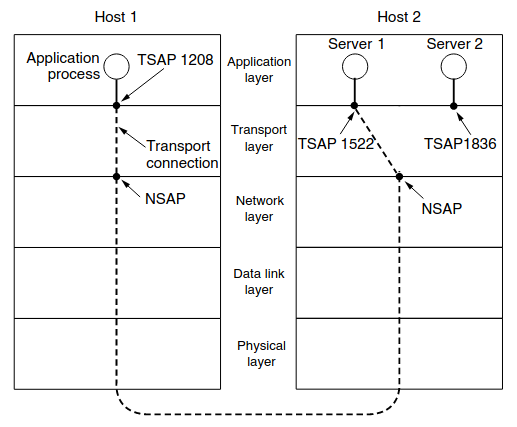
\includegraphics[width=0.85\textwidth]{gambar/TSAPs_NSAPs_and_transport_connections}
  \caption{Koneksi Transportasi TSAP dan NSAP}
\end{figure}

\emph{Application process}, baik klien maupun server, dapat melampirkan dirinya sendiri ke TSAP lokal untuk membuat sambungan ke TSAP jarak jauh. Koneksi ini dijalankan melalui NSAP pada setiap \emph{host}. Tujuan dari memiliki TSAP adalah bahwa di beberapa jaringan, setiap komputer memiliki NSAP tunggal, jadi beberapa cara diperlukan untuk membedakan beberapa titik akhir transportasi yang berbagi itu NSAP. Skenario yang mungkin untuk koneksi transportasi adalah sebagai berikut:

\begin{enumerate}
  \item{Proses server email menempel pada TSAP 1522 di \emph{host} 2 untuk menunggu panggilan masuk atau \emph{incoming call}. Bagaimana suatu proses menempel pada TSAP berada di luar model jaringan dan sepenuhnya bergantung pada operasi sistem lokal. Panggilan seperti \emph{LISTEN} dapat digunakan.}

  \item{\emph{Application Process} pada \emph{host} 1 ingin mengirim pesan email, jadi itu menempel pada TSAP 1208 dan mengeluarkan permintaan \emph{CONNECT}. Permintaan yang menentukan TSAP 1208 pada \emph{host} 1 sebagai sumber dan TSAP 1522 pada \emph{host} 2 sebagai tujuan. Tindakan ini pada akhirnya menghasilkan koneksi transportasi yang dibuat antara \emph{application process} dan server.}

  \item{\emph{Application process} mengirim \emph{mail message}.}

  \item{\emph{Mail server} merespon kalau pesan itu akan dikirimkan.}

  \item{Koneksi transportasi dilepaskan.}
\end{enumerate}

\emph{Multiplexing}, atau berbagi beberapa percakapan melalui koneksi, \emph{virtual circuits}, dan \emph{physical link} berperan dalam beberapa lapisan arsitektur jaringan. Pada lapisan transportasi, kebutuhan akan \emph{multiplexing} dapat muncul dalam beberapa cara. Jika hanya satu alamat jaringan yang tersedia di sebuah \emph{host}, semua koneksi transportasi pada perangkat harus menggunakannya. Ketika sebuah segmen masuk, ada caranya diperlukan untuk mengetahui proses mana yang harus diberikan. Situasi ini, disebut \emph{multiplexing}.

\begin{figure}[H]
  \centering{}
	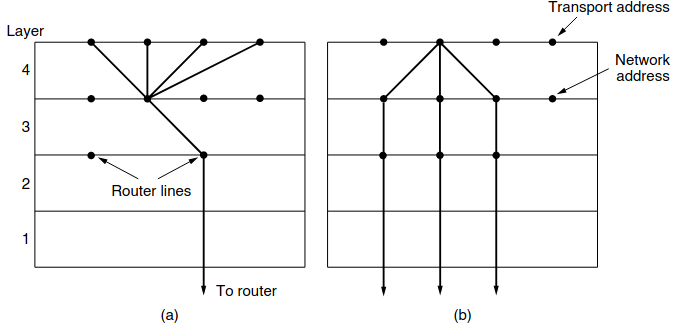
\includegraphics[width=0.85\textwidth]{gambar/multiplexing}
  \caption{(a) Multiplexing, (b) Inverse Multiplexing}
\end{figure}

\emph{Multiplexing} juga berguna di lapisan transport karena alasan lain. Misalkan, sebuah \emph{host} memiliki banyak jalur jaringan yang dapat digunakannya. Jika pengguna membutuhkan lebih banyak \emph{bandwidth} atau lebih banyak \emph{reliability} daripada yang dapat disediakan oleh salah satu jalur jaringan, jalan keluarnya adalah memiliki koneksi yang mendistribusikan lalu lintas di antara banyak jalur jaringan dengan basis \emph{round-robin}, seperti ditunjukkan pada Gambar 2.7 (b). Modus operandi disebut \emph{inverse multiplexing}. Dengan k koneksi jaringan terbuka, \emph{bandwidth} efektif dapat ditingkatkan dengan faktor k. Contoh \emph{inverse multiplexing} adalah SCTP (\emph{Stream Control Transmission Protocol}) yang dapat menjalankan koneksi menggunakan beberapa antarmuka jaringan. Sebaliknya, TCP menggunakan titik akhir jaringan tunggal. \emph{Inverse multiplexing} juga ditemukan pada lapisan \emph{link}, ketika beberapa \emph{low-rate links} digunakan secara paralel sebagai satu tautan cepat.

\subsubsection{\emph{User Datagram Protocol}}

Paket protokol internet mendukung protokol transportasi \emph{connectionless} yang disebut UDP. UDP menyediakan cara bagi aplikasi untuk mengirim enkapsulasi datagram IP tanpa harus membuat koneksi. UDP mentransmisikan segmen yang terdiri dari \emph{header} 8-byte diikuti oleh \emph{payload}. Pada Gambar 2.8, ada \emph{port} yang berfungsi untuk mengidentifikasi titik dalam perangkat sumber dan tujuan. Ketika paket UDP tiba, \emph{payload} diserahkan ke proses yang melekat pada \emph{port} tujuan. Lampiran ini terjadi ketika primitif \emph{BIND} atau yang serupa digunakan.

\begin{figure}[H]
  \centering{}
	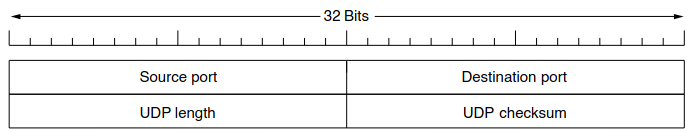
\includegraphics[width=0.85\textwidth]{gambar/the_UDP_header}
  \caption{UDP Header}
\end{figure}

\emph{Port} sumber sangat dibutuhkan ketika balasan harus dikirim kembali ke sumber. Dengan menyalin bidang \emph{port} sumber dari \emph{incoming segment} ke bidang \emph{port} tujuan dari \emph{outgoing segment}, proses pengiriman balasan dapat menentukan proses mana pada perangkat pengirim yang akan menerimanya. Bidang panjang UDP menyertakan \emph{header} 8-byte dan data. Minimal panjangnya 8 byte, untuk menutupi \emph{header}. Panjang maksimumnya adalah 65.515 byte, yang lebih rendah dari jumlah terbesar yang muat dalam 16-bit karena batas ukuran pada paket IP.

\emph{Checksum opsional} juga disediakan untuk keandalan ekstra. Melakukan \emph{checksum  header}, data, dan \emph{conceptual IP pseudoheader}. Saat melakukan perhitungan ini, \emph{Checksum field} disetel ke nol dan bidang data diisi dengan byte nol tambahan jika panjangnya adalah angka ganjil. Algoritma \emph{checksum} hanya menjumlahkan semua kata 16-bit dalam komplemen satu dan mengambil komplemen dari jumlah tersebut. Konsekuensinya, saat penerima melakukan perhitungan pada seluruh segmen, termasuk \emph{checksum field}, hasilnya harus 0. Jika \emph{checksum} tidak dihitung, disimpan sebagai 0, 0 yang benar dihitung disimpan sebagai semua 1.

\emph{Pseudoheader} untuk kasus IPv4 ditunjukkan pada Gambar 2.9. Berisi alamat IPv4 32-bit dari perangkat sumber dan tujuan, nomor protokol untuk UDP (17), dan jumlah byte untuk segmen UDP (termasuk header). Menyertakan \emph{pseudoheader} dalam komputasi \emph{checksum} UDP membantu mendeteksi paket yang salah kirim, tetapi menyertakannya juga melanggar hierarki protokol karena alamat IP di dalamnya milik lapisan IP, bukan milik lapisan UDP. TCP menggunakan \emph{pseudoheader} yang sama untuk \emph{checksum}-nya.

\begin{figure}[H]
  \centering{}
	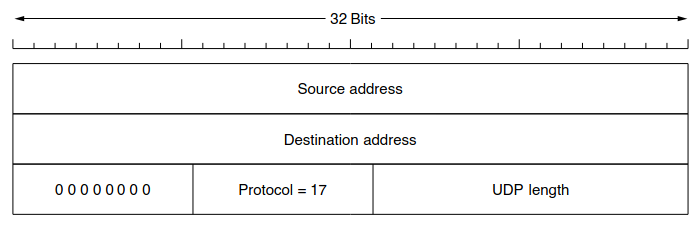
\includegraphics[width=0.85\textwidth]{gambar/the_IPv4_pseudoheader_included_in_the_UDP_checksum}
  \caption{IPv4 Pseudoheader di UDP Checksum}
\end{figure}

% Informasi dapat diangkut dari penelepon ke penerima dalam parameter dan dapat kembali dalam hasil prosedur. Tidak ada pesan yang lewat terlihat oleh pemrogram aplikasi. Teknik ini dikenal sebagai RPC (\emph{Remote Procedure Call}) dan telah menjadi dasar bagi banyak aplikasi jaringan. Secara tradisional, prosedur pemanggilan dikenal sebagai klien dan prosedur yang dipanggil dikenal sebagai server. Ide di balik RPC adalah membuat panggilan prosedur jarak jauh terlihat semirip mungkin dengan panggilan lokal. Dalam bentuk paling sederhana, untuk memanggil prosedur jarak jauh, klien program harus terikat dengan prosedur library kecil, yang disebut klien stub, mewakili prosedur server di ruang alamat klien. Begitu pula dengan server terikat dengan prosedur yang disebut rintisan server stub. Prosedur ini menyembunyikan fakta bahwa panggilan prosedur dari klien ke server bukan lokal.

% RPC \emph{client-server} adalah salah satu area di mana UDP digunakan secara luas. Satu lagi adalah untuk aplikasi multimedia real-time. Secara khusus, karena radio internet, telepon Internet, musik sesuai permintaan, konferensi video, video sesuai permintaan, dan aplikasi multimedia lainnya menjadi lebih umum, orang telah menemukan bahwa masing-masing aplikasi menciptakan kembali protokol transportasi real-time yang kurang lebih sama. Dia secara bertahap menjadi jelas bahwa memiliki protokol transport real-time umum untuk beberapa aplikasi merupakan ide yang bagus. Maka lahirlah RTP (Real-time Transport Protocol). Terdapat dua aspek transportasi real-time. Yang pertama adalah protokol RTP untuk transportasi data audio dan video dalam paket. Yang kedua adalah proses yang terjadi,
% sebagian besar di penerima, untuk memutar audio dan video pada waktu yang tepat.

\subsubsection{\emph{User Datagram Protocol}}

TCP dirancang khusus untuk menyediakan aliran byte end-to-end melalui \emph{unreliable internetwork}. Sebuah jaringan internet berbeda dari satu jaringan karena bagian yang berbeda mungkin sangat berbeda topologi, \emph{bandwidth}, \emph{delays}, ukuran paket, dan parameter lainnya. TCP dulu dirancang untuk secara dinamis beradaptasi dengan properti dari \emph{internetwork} dan menjadi kuat menghadapi berbagai macam kegagalan. Layanan TCP diperoleh oleh pengirim dan penerima yang menciptakan akhir poin, disebut socket. Setiap socket memiliki nomor socket (alamat) yang terdiri dari alamat IP \emph{host} dan nomor 16-bit lokal ke \emph{host} tersebut, yang disebut \emph{port}. \emph{Port} adalah nama TCP untuk TSAP. Agar layanan TCP menjadi diperoleh, koneksi harus dibuat secara eksplisit antara socket pada satu perangkat dan di perangkat yang lain. Socket dapat digunakan untuk beberapa koneksi sekaligus. 

Nomor \emph{port} di bawah 1024 dicadangkan untuk layanan standar yang biasanya bisa hanya dapat dimulai oleh \emph{privileged users}. Disebut sebagai \emph{well-known} \emph{ports}. Berikut adalah contoh dari beberapa \emph{port} yang sudah digunakan.

\break
\begin{center}
  \begin{longtable}{ |P{0.25\textwidth{}} |P{0.25\textwidth{}} |P{0.25\textwidth{}}|}
    \caption{\textit{Well-known ports}
    % \ref{tab:lirik}
    }
    % \label{tab:word_index} 
    \\
    \hline{}
    \textbf{Port} & \textbf{Protokol} & \textbf{Kegunaan} \\
    \hline{}
    20, 21 & FTP & File transfer\\
    \hline{}
    22 & SSH & Remote login, pengganti untuk Telnet \\
    \hline{}
    25 & SMTP & Email \\
    \hline{}
    80 & HTTP & World Wide Web \\
    \hline{}
    110 & POP-3 & Remote email access \\
    \hline{}
    143 & IMAP & Remote email access \\
    \hline{}
    443 & HTTPS & Secure Web (HTTPS) \\
    \hline
  \end{longtable}
\end{center}

Semua koneksi TCP adalah \emph{full duplex} dan \emph{point-to-point}. \emph{Full duplex} berarti bahwa lalu lintas dapat berjalan di kedua arah secara bersamaan. \emph{Point-to-point} artinya setiap koneksi memiliki tepat dua titik akhir. TCP tidak mendukung \emph{multicasting} atau \emph{broadcasting}. Koneksi TCP adalah \emph{byte stream}, bukan \emph{message stream}. \emph{Message boundaries} tidak dipertahankan dari ujung ke ujung.

Fitur utama dari TCP, dan yang mendominasi desain protokol, adalah bahwa setiap byte pada koneksi TCP memiliki nomor urut 32-bit sendiri. Ketika internet dimulai, jalur antar router sebagian besar adalah 56-kbps \emph{leased line}, jadi \emph{host} membutuhkan waktu lebih dari 1 minggu untuk menggilir nomor urut. Pada kecepatan jaringan modern, nomor urut dapat dikonsumsi dengan \emph{alarming rate}. Nomor urut 32-bit yang terpisah dibawa pada paket untuk posisi \emph{sliding window} dalam satu arah dan untuk \emph{acknowledgement} dalam arah sebaliknya. 

Entitas TCP pengirim dan penerima bertukar data dalam bentuk segmen. Segmen TCP terdiri dari header 20-byte tetap (ditambah bagian opsional) yang diikuti dengan nol atau lebih byte data. Perangkat lunak TCP memutuskan seberapa besar seharusnya segmen menjadi. Itu dapat mengumpulkan data dari beberapa penulisan menjadi satu segmen atau dapat membagi data dari satu penulisan ke beberapa segmen. Dua batasan membatasi ukuran segmen. Pertama, setiap segmen, termasuk header TCP, harus sesuai dengan muatan IP 65.515 byte. Kedua, setiap link memiliki MTU (\emph{Maximum Transfer Unit}). Setiap segmen harus muat di MTU di pengirim dan penerima sehingga dapat dikirim dan diterima di paket tunggal yang tidak terfragmentasi. Dalam praktiknya, MTU umumnya berukuran 1500 byte.

\begin{figure}[H]
  \centering{}
	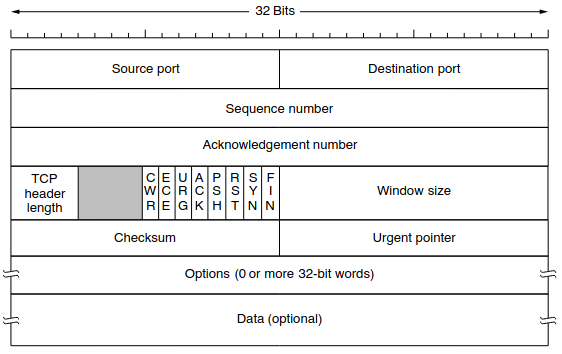
\includegraphics[width=0.85\textwidth]{gambar/the_TCP_header}
  \caption{TCP Header}
\end{figure}

% Panjang header TCP memberi tahu berapa banyak kata 32-bit yang terkandung dalam header TCP. Informasi ini diperlukan karena bidang Options memiliki panjang variabel, jadi header-nya juga. Secara teknis, bidang ini benar-benar menunjukkan awal dari data dalam segmen, diukur dalam kata 32-bit, tetapi angka itu hanyalah panjang header, jadi efeknya sama.

\subsection{\emph{Application Layer}}

Pada lapisan ini mengandung \emph{higher-level protocol}: \emph{virtual terminal} (TELNET), file transfer (FTP), \emph{electronic mail} (SMTP), dan \emph{Domain Name System} (DNS). Hilangnya lapisan \emph{session} dan presentation disatukan pada lapisan application, jadi tidak semata - mata hilang begitu saja. Karena kedua lapisan tersebut tidak banyak berguna untuk sebagian besar aplikasi, oleh karena itu dihilangkan. Pada lapisan ini secara langsung memberikan layanan kepada pengguna seperti menggunakan internet, melakukan operasi pada perangkat lunak, dan kegiatan lainnya.

\subsubsection{\emph{World Wide Web}}

\emph{World Wide Web} (WWW) adalah arsitektur kerangka kerja untuk mengakses konten tertaut yang tersebar lebih dari jutaan mesin melalui internet. Web dimulai pada tahun 1989 di CERN (Conseil Européen pour la Recherche Nucléaire), Pusat Riset Nuklir Eropa. Ide awalnya adalah untuk membantu tim besar, seringkali dengan anggota yang banyak atau banyak negara dan zona waktu, berkolaborasi menggunakan koleksi yang terus berubah laporan, cetak biru, gambar, foto, dan dokumen lain yang dihasilkan oleh eksperimen dalam fisika partikel. Proposal untuk Web dokumen tertaut berasal fisikawan CERN Tim Berners-Lee. Prototipe pertama (berbasis teks) telah beroperasi 18 bulan kemudian. Demonstrasi publik yang diberikan pada konferensi Hypertext '91 menarik perhatian peneliti lain, yang membuat Marc Andreessen di University of Illinois mengembangkan browser grafis pertama. Itu disebut Mosaic dan dirilis pada Februari 1993.

Dari sudut pandang pengguna, Web terdiri dari koleksi yang luas dan mendunia dalam bentuk halaman web. Setiap halaman biasanya berisi tautan ke ratusan objek lain, yang dapat di-\emph{hosting} di server mana pun di internet, di mana pun di dunia. Objek - objek ini mungkin berupa teks dan gambar lain, tetapi saat ini juga menyertakan berbagai macam objek, termasuk iklan dan skrip pelacakan. Halaman juga dapat ditautkan ke halaman web lain; pengguna dapat mengikuti tautan dengan mengkliknya, yang kemudian membawa mereka ke halaman yang ditunjuk. Proses ini dapat diulang tanpa batas. Gagasan memiliki satu halaman menunjuk ke yang lain, sekarang disebut hypertext, ditemukan oleh M.I.T. profesor teknik elektro, Vannevar Bush, pada tahun 1945. Ini jauh sebelum internet ditemukan. 

\subsubsection{\emph{Content and Internet Traffic}}

Internet digunakan untuk semua tentang komunikasi \emph{point-to-point}, seperti jaringan telepon. Banyak orang telah menggunakan email untuk berkomunikasi satu sama lain sejak lama, dan sekarang menggunakan video dan \emph{voice over} IP. Namun, sejak web tumbuh, internet telah menjadi lebih dari sekadar tentang konten daripada komunikasi. Banyak orang menggunakan Web untuk mencari informasi, dan ada banyak sekali pengunduhan musik, video, dan materi lainnya. Karena tugas mendistribusikan konten berbeda dengan \emph{point-to-point} komunikasi, itu menempatkan persyaratan yang berbeda pada jaringan.

Teknik yang digunakan untuk distribusi konten telah berkembang dalam waktu ke waktu. Di awal pertumbuhan web, popularitasnya hampir berakhir. Lagi permintaan konten menyebabkan server dan jaringan sering kelebihan beban. Banyak orang mulai menyebut WWW sebagai \emph{World Wide Wait}. Untuk mengurangi penundaan tidak berujung, para peneliti mengembangkan arsitektur yang berbeda untuk menggunakan \emph{bandwidth} untuk mendistribusikan konten. Arsitektur umum untuk mendistribusikan arsitektur konten adalah CDN (\emph{Content Delivery Network}), terkadang juga disebut \emph{Content Distribution Network}. CDN secara efektif adalah kumpulan \emph{cache} terdistribusi yang sangat besar, yang biasanya berfungsi konten langsung ke klien. Cara lain untuk mendistribusikan konten adalah melalui jaringan P2P (\emph{Peer-to-Peer}), di mana komputer saling menyajikan konten, biasanya tanpa penyediaan terpisah pada server atau titik pusat kontrol apa pun. 

CDN mengubah gagasan \emph{caching web} tradisional. Alih-alih meminta klien mencari salinan halaman yang diminta di \emph{cache} terdekat, provider menempatkan salinan halaman dalam satu set node di lokasi yang berbeda dan mengarahkan klien untuk menggunakan node terdekat sebagai server.

\begin{figure}[H]
  \centering{}
	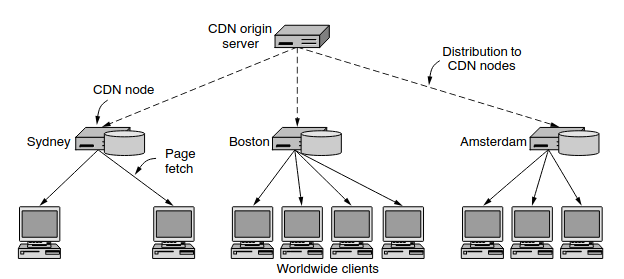
\includegraphics[width=0.85\textwidth]{gambar/CDN_distribution_tree}
  \caption{CDN Tree}
\end{figure}

Menggunakan \emph{tree stucture} memiliki tiga keuntungan. Pertama, distribusi konten bisa ditingkatkan ke klien sebanyak yang diperlukan dengan menggunakan lebih banyak \emph{node} di CDN, dan lebih banyak level di pohon saat distribusi di antara \emph{node} CDN menjadi hambatan. Tidak peduli berapa banyak klien yang ada, struktur pohonnya efisien. \emph{Origin server} tidak kelebihan beban karena berbicara ke banyak klien melalui pohon \emph{node} CDN, tidak harus menjawab setiap permintaan untuk sebuah halaman dengan sendirinya. Kedua, setiap klien mendapatkan kinerja yang baik dengan mengambil halaman dari server terdekat dibanding server yang jauh. Ini karena waktu bolak-balik untuk menyiapkan koneksi lebih pendek, lambat laun TCP meningkat lebih cepat karena perjalanan bolak-balik dengan waktu yang lebih pendek, dan jalur jaringan yang lebih pendek cenderung melewati daerah kemacetan di internet. Terakhir, total beban yang ditempatkan di jaringan juga disimpan secara minimal. Jika \emph{node} CDN ditempatkan dengan baik, lalu lintas untuk halaman tertentu harus melewati setiap bagian dari jaringan hanya sekali.

\subsubsection{\emph{Peer-to-Peer Network}}

Ide dasar dari jaringan berbagi file P2P adalah bahwa banyak komputer bersatu dan menyatukan sumber daya mereka untuk membentuk sistem distribusi konten. Komputer seringkali hanya komputer rumahan. Mereka tidak perlu seperti mesin di pusat data internet. Komputer disebut rekan atau \emph{peers} karena masing - masing seseorang dapat secara bergantian bertindak sebagai klien ke \emph{peer} lain, mengambil kontennya, dan sebagai server, menyediakan konten ke \emph{peer} lain. Apa yang membuat sistem \emph{peer-to-peer} menarik adalah bahwa tidak ada infrastruktur khusus, tidak seperti di CDN. Semua orang berpartisipasi dalam tugas mendistribusikan konten, dan seringkali tidak ada titik pusat kendali. Banyak orang yang tertarik dengan teknologi P2P. Alasannya bukan karena dibutuhkan perusahaan besar untuk menjalankan CDN, sementara siapa pun yang memiliki komputer dapat bergabung dengan jaringan P2P. Jaringan P2P yang memiliki kapasitas yang luar biasa untuk mendistribusikan konten.

Protokol BitTorrent dikembangkan oleh Bram Cohen pada tahun 2001 untuk memungkinkan satu set \emph{peer} berbagi file dengan cepat dan mudah. Ada banyak klien yang tersedia secara bebas yang menggunakan protokol ini, sama seperti banyak \emph{browser} yang menggunakan protokol HTTP ke \emph{web server}. Terdapat tiga masalah yang harus selesaikan dalam hal membagikan konten ini: bagaimana caranya agar \emph{peer} dapat mencari \emph{peer} lainnya ketika ingin mengunduh konten?, bagaimana konten dapat direplikasi oleh \emph{peer} untuk menyediakan kecepatan mengunduh untuk semua orang?, dan bagaimana untuk mendorong sesama \emph{peer} untuk mengunggah konten ke orang lain seperti mengunduh konten untuk diri mereka sendiri?

Masalah pertama ada karena tidak semua \emph{peer} akan memiliki semua konten. Itu pendekatan yang diambil di BitTorrent adalah untuk setiap penyedia konten untuk membuat konten deskripsi disebut torrent. Torrent jauh lebih kecil dari kontennya, dan memang demikian digunakan oleh \emph{peer} untuk memverifikasi integritas data yang diunduh dari \emph{peer} lain. Pengguna lain yang ingin mengunduh konten harus mendapatkan torrent terlebih dahulu.

\begin{figure}[H]
  \centering{}
	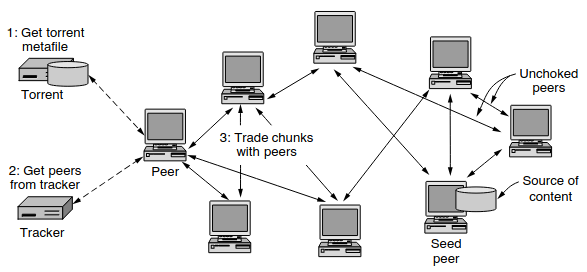
\includegraphics[width=0.85\textwidth]{gambar/BitTorrent}
  \caption{Bittorent}
\end{figure}

Masalah kedua adalah bagaimana berbagi konten dengan cara yang memberikan unduhan cepat. Kumpulan \emph{peer} disebut \emph{swarm}. Saat \emph{swarm} pertama kali terbentuk, beberapa \emph{peer} harus memiliki semua bongkahan itu buat isinya. \emph{Peer} ini disebut seeder. \emph{Peer} lainnya yang bergabung dengan \emph{swarm} tidak akan memiliki \emph{chunks},  \emph{peer} yang mengunduh konten. Sementara \emph{peer} yang berpartisipasi dalam \emph{swarm}, secara bersamaan mengunduh \emph{chunks} yang hilang dari \emph{peer} lain, dan mengunggah potongan yang dimilikinya ke \emph{peer} lain yang membutuhkan. \emph{Trading} ini ditunjukan pada tahap ketiga dari Gambar 2.12. Seiring waktu, \emph{peer} mengumpulkan lebih banyak \emph{chunk} hingga semuanya berhasil diunduh. \emph{Peer} dapat meninggalkan \emph{swarm} kapan saja. Biasanya \emph{peer} akan tinggal untuk waktu yang singkat setelah menyelesaikan unduhannya sendiri. Dengan \emph{peers} yang datang dan pergi, tingkat \emph{chunk} dalam \emph{swarm} bisa sangat tinggi.

Masalah ketiga melibatkan insentif. \emph{Node} CDN diatur secara eksklusif untuk memberikan konten kepada pengguna. \emph{Node} P2P tidak. Mereka adalah komputer pengguna, dan pengguna mungkin lebih tertarik untuk mendapatkan konten daripada membantu unduhan pengguna lain, dengan kata lain, terkadang ada insentif bagi pengguna untuk menipu sistem. \emph{Node} yang mengambil sumber daya dari suatu sistem tanpa memberikan kontribusi dalam bentuk apa pun adalah disebut \emph{free-rider} atau \emph{leechers}. Jika jumlahnya terlalu banyak, sistem tidak akan berfungsi dengan baik. BitTorrent berupaya mengatasi masalah ini dengan memberi penghargaan kepada \emph{peers} yang menunjukkan perilaku pengunggahan yang baik. Setiap {peer} secara acak mengambil sampel {peer} lainnya, mengambil chunk dari mereka saat mengunggah potongan ke mereka. {Peer} terus \emph{trading chunk} dengan hanya sejumlah kecil {peer} yang memberikan kinerja unduhan tertinggi, sementara juga secara acak mencoba {peer} lain untuk menemukan mitra yang baik. Secara acak mencoba {peer} juga memungkinkan pendatang baru untuk mendapatkan chunk awal yang dapat mereka \emph{trading} dengan {peer} lainnya. {Peers} yang saat ini bertukar chunk disebut unchoked.

\section{\emph{Hypertext Transfer Protocol}}

\emph{Hypertext Transfer Protocol} (HTTP) adalah sebuah protokol yang terdapat pada lapisan \emph{application} yang terdapat pada TCP/IP model. Melalui HTTP, data klien dapat meminta data kepada server dan server dapat mengirimkan kembali datanya. Data yang dikirim dapat berupa text, text layout, gambar, dll.

\subsection{\emph{HTTP/2}}

Sejak awal pembuatan HTTP/2 pada tahun 2012 dilakukan karena HTTP/1.0 dan HTTP/1.1 sudah terbentuk sejak 2007 dan sudah cukup lama. Oleh karena itu, \emph{Internet Engineering Task Force} (IETF) membentuk grup untuk membuat HTTP/2. Grup ini memiliki beberapa tujuan: mengizinkan klien dan server untuk memilih versi HTTP yang akan digunakan, menjaga kompatibilitas dengan HTTP/1.1 sebaik mungkin, meningkatkan performa dengan \emph{multiplexing}, \emph{pipelining}, \emph{compression}, dll, serta mendukung \emph{browsers}, \emph{servers}, \emph{proxies}, \emph{delivery}, jaringan yang sudah ada agar dapat menggunakan versi terbaru dari HTTP.

HTTP/2 lebih unggul dalam hal kecepatan browsing web dikarenakan ketika klien meminta data dari server, data tersebut dapat dikirim dalam bentuk \emph{binary} dan sistem koneksi yang dibuat dapat meminta banyak data dan dapat dikirimkan dengan urutan yang diinginkan, karena berjalan secara \emph{multiplexing}. Tanpa harus meminta data satu persatu, seperti yang terdapat pada HTTP/1.1.

Kendala enkripsi menjadi suatu perdebatan pada HTTP/2. Dikarenakan banyak pihak yang sangat menginginkannya, tetapi banyak juga pihak yang menolaknya. Sebagian besar yang menolak hal tersebut adalah yang berkaitan dengan \emph{Internet-of-Things} (IoT). Karena pada bidang IoT, enkripsi tidak dibutuhkan. Tetapi pada semua \emph{browsers} memerlukan enkripsi, pada akhirnya tetap ada enkripsi untuk keperluan web \emph{browsing}.

\subsection{\emph{HTTP/3}}

HTTP/3 adalah revisi terbesar ketiga dari HTTP, didesain sebagai penerus dari HTTP/2. Perbedaan terbesar dari HTTP/3 adalah pada lapisan transportasi yang mendukung HTTP \emph{messages} ketimbang bergantung pada TCP. Karena sekarang mendukung Quick UDP Internet Connections (QUIC) yang merupakan versi tambahan dari UDP. Sudah banyak bahasa pemrograman yang mendukung penggunaan QUIC dan HTTP/3 seperti C, C++, Python, Rust, dan Go. \emph{Web server} nginx juga sudah memadai untuk HTTP/3.

Pada HTTP/3 juga masih menggunakan layanan yang sama dengan HTTP/2 seperti \emph{multiplexing}. QUIC memiliki pengaturan koneksi \emph{zero-round-trip}, ketika koneksi sudah tersedia di \emph{server endpoint} atau sebelumnya klien sudah pernah terhubung ke suatu server, HTTP/3 dapat mengizinkan klien untuk menggunakan kembali koneksi tersebut dengan berbagai macam URLs yang berbeda dan secara cepat. Karena HTTP/3 berjalan di atas QUIC yang merupakan lapisan transportasi akan meningkatkan performa yang sangat signifikan. Dengan kata lain, QUIC adalah generasi selanjutnya dari TCP.

% \section{\emph{Quick UDP Internet Connection}}

% Quick UDP Internet Connections (QUIC) adalah desain transport baru yang akan meningkatkan performa dari HTTPS traffic. QUIC support ditambahkan ke Chrome pada Juni 2013. Setelah tahap eksperimental, QUIC terbukti stabil dan aman dan sejak Januari 2017, QUIC diaktifkan untuk hampir semua pengguna Chrome dan aplikasi YouTube Android. Berawal dari perkembangan layanan web, latensi merupakan suatu hal yang menjadi penghalang dalam pengalaman pengguna dalam menggunakan aplikasi. Upaya untuk mengurangi latensi di bagian mekanisme transport umumnya mengalami fundamental keterbatasan ekosistem TLS/TCP. Dengan dikembangkannya QUIC ada bentuk upaya dan motivasi untuk mengurangi latensi tersebut.

% Dengan proses perkembangan QUIC mendorong untuk perkembangan dari transport protocol. Protokol transport TCP telah memenuhi permintaan aplikasi yang berkembang di luar layanan sederhana TCP dan belum ada penerapan yang luas. Middlebox sekarang menjadi faktor penting dalam arsitektur internet. Middlebox adalah perangkat jaringan komputer yang dapat memeriksa, memfilter, dan memodifikasi traffic dari internet. Contohnya seperti firewall. Middlebox bertujuan untuk meningkatkan keamanan dan performa internet. Firewall cenderung untuk memblokir apapun yang tidak biasa untuk alasan keamanan dan Network Address Translators (NATs) menulis ulang transport header. Sehingga tidak mampu memberikan izin traffic dari protokol transport yang baru tanpa menambahkan konfigurasi dukungan. Banyak packet content yang tidak dilindungi keamanan secara end-to-end, seperti TCP packet header. Oleh karena itu, middlebox berhak untuk memeriksa dan memodifikasi. Melakukan perubahan ke TCP sudah mencapai titik yang keuntungan yang semakin sedikit.

% Perkembangan internet yang pesat juga diiringi dengan perkembangan ancaman terhadap keamanannya dalam berbagai hal, termasuk transport. Perlu ada perubahan yang sangat masif dari sisi client. TCP diimplementasikan pada kernel Operating System (OS), biasanya untuk memodifikasi TCP diperlukan peningkatan OS terlebih dahulu. Untuk perubahan dengan skala besar akan memakan banyak waktu. Terdapatnya handshake delay ketika koneksi ingin dibuat antara client dan server pada HTTPS stack membuat cost yang mahal pada TCP. Sebagian besar koneksi di Internet, dan tentunya sebagian besar kegiatan aktif web adalah short transfer dan paling terpengaruh oleh yang kegiatan handshake round trips yang tidak perlu. Untuk mengurangi latensi dan cost yang besar HTTP/1 membatasi jumlah koneksi yang dibuat antara client dan server. Pada HTTP/2 dikenalkan multiplexes. Secara menyeluruh, untuk memodifikasi transport diperlukan perubahan pada web servers dan clients. Terkadang juga terintervensi dengan middlebox. Menerapkan perubahan pada ketiga komponen memerlukan insentif dan koordinasi antara pengembang aplikasi, OS vendor, vendor middlebox, dan operator jaringan yang mengembangkan middlebox ini. QUIC mengenkripsi header dan build transport function di atas UDP, menghindari ketergantungan pada vendor dan operator jaringan dan memindahkan kontrol pengembangan transportasi ke aplikasi yang mendapat manfaat langsung.

\nocite{tanenbaum2021computer}

\section{\emph{Socket Programming}}

Socket pertama kali dirilis sebagai bagian dari Berkeley UNIX 4.2BSD distribusi perangkat lunak pada tahun 1983. Socket dengan cepat menjadi populer. \emph{Primitives} itu sekarang digunakan untuk pemrograman internet pada banyak sistem operasi, terutama sistem berbasis UNIX, dan ada API (\emph{Application Programming Interface}) bergaya socket untuk Windows disebut `winsock.'

\begin{figure}[H]
  \centering{}
	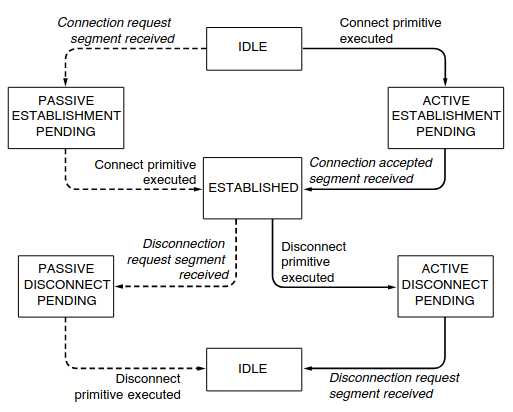
\includegraphics[width=0.85\textwidth]{gambar/a_state_diagram_for_a_simple_connection_management_scheme}
  \caption{Skema Koneksi Manajemen Sederhana}
\end{figure}

Pada Gambar 2.13 koneksi manajemen yang sederhana dengan model yang memiliki lebih banyak fitur dan fleksibel. Terdapat beberapa \emph{primitives} yang terlampir pada skema tersebut.

\begin{center}
  \begin{longtable}{ |P{0.2\textwidth{}} |P{0.3\textwidth{}} |P{0.3\textwidth{}}|}
    \caption{\textit{Primitive} pada \textit{Socket}
    % \ref{tab:lirik}
    }
    % \label{tab:word_index} 
    \\
    \hline{}
    \textbf{\textit{Primitive}} & \textbf{Berarti} \\
    \hline{}
    \emph{SOCKET} & Membuat sebuah komunikasi endpoint baru  \\
    \hline{}
    \emph{BIND} & Mengasosiasi alamat lokal dengan socket \\
    \hline{}
    \emph{LISTEN} & Bersedia untuk menerima koneksi dan membuat antrian \\
    \hline{}
    \emph{ACCEPT} & Mengizinkan koneksi masuk dan terbentuk secara pasif \\
    \hline{}
    \emph{CONNECT} & Melakukan percobaan untuk mendirikan koneksi secara aktif \\
    \hline{}
    \emph{SEND} & Mengirimkan beberapa data melalui koneksi \\
    \hline{}
    \emph{RECEIVE} & Menerima beberapa data dari koneksi  \\
    \hline{}
    \emph{CLOSE} & Melepaskan koneksi  \\
    \hline
  \end{longtable}
\end{center}

Empat \emph{primitives} pertama dalam daftar dieksekusi dalam urutan oleh server. SOCKET \emph{primitive} membuat titik akhir baru dan mengalokasikan ruang tabel untuknya di dalam entitas transportasi. Parameter panggilan menentukan format pengalamatan yang akan digunakan, jenis layanan yang diinginkan (misalnya \emph{reliable byte stream}), dan protokol. Panggilan socket yang berhasil mengembalikan \emph{file descriptor} biasa untuk digunakan dalam panggilan yang berhasil, sama seperti panggilan \emph{OPEN} pada file.

Socket yang baru dibuat tidak memiliki alamat jaringan. Oleh karena itu, menggunakan \emph{BIND}. Setelah server mengikat alamat ke socket, klien jarak jauh dapat terhubung ke sana. Berikutnya adalah panggilan \emph{LISTEN}, yang mengalokasikan ruang untuk mengantri panggilan, jika terdapat beberapa klien yang mencoba untuk terhubung pada waktu yang sama. Ketika segmen yang meminta koneksi tiba, entitas transportasi membuat socket baru dengan properti yang sama dengan yang asli dan mengembalikan \emph{file descriptor} untuk itu. Server kemudian dapat memotong proses atau utas untuk menangani koneksi pada socket baru dan kembali menunggu koneksi berikutnya pada socket asli. \emph{ACCEPT} mengembalikan \emph{file descriptor}, yang dapat digunakan untuk membaca dan menulis dengan cara standar, sama seperti untuk file.

CONNECT memblokir pemanggil dan memulai proses koneksi. Ketika segmen yang sesuai diterima dari server, proses klien dibuka blokirnya dan koneksi dibuat. Kedua belah pihak sekarang dapat menggunakan \emph{SEND} dan \emph{RECEIVE} untuk mengirim dan menerima data melalui koneksi full-duplex. Panggilan sistem UNIX \emph{READ} dan \emph{WRITE} standar juga dapat digunakan jika tidak ada opsi khusus \emph{SEND} dan \emph{RECEIVE} yang diperlukan. Pelepasan koneksi dengan socket bersifat simetris. Ketika kedua belah pihak telah mengeksekusi \emph{CLOSE}, sambungan dilepaskan atau dihentikan.

Berikut adalah penjelasan terkait bagaimana penerapan sederhana socket dilakukan. Kodenya akan memiliki beberapa batasan, tetapi telah menerapkan prinsip dasar socket dan dapat dikompilasi oleh berbagai sistem UNIX yang terhubung ke internet. Kode klien dapat dieksekusi dengan parameter yang sesuai untuk mengambil file apapun pada server yang memiliki akses pada mesinnya. 

Kode server dimulai dengan memasukkan beberapa standar \emph{header}, tiga yang terakhir berisi definisi terkait internet utama dan struktur data. Berikutnya adalah definisi \emph{SERVER\_PORT} sebagai 8080. Angka ini dipilih secara bebas. Angka apa pun antara 1024 dan 65535 akan berfungsi sama baik, selama tidak digunakan oleh beberapa proses lain, \emph{port} di bawah 1023 dicadangkan untuk \emph{privileged users}. Dua baris berikutnya di server mendefinisikan konstanta. Yang pertama menentukan ukuran potongan dalam byte yang digunakan untuk transfer file. Yang kedua menentukan bagaimana banyak koneksi yang tertunda dapat ditahan sebelum koneksi tambahan dibuang.

Setelah deklarasi variabel lokal, kode server dimulai. Dimulai dengan menginisialisasi struktur data yang akan menyimpan alamat IP server. Struktur data ini akan segera terikat ke socket server. Memanggil \emph{memset} mengatur data struktur untuk semua menjadi 0s. Tiga tugas berikutnya mengisi tiga bidangnya. Terakhir berisi \emph{port} server. Fungsi htonl dan htons harus dilakukan dengan mengkonversi nilai ke format standar sehingga kode berjalan dengan benar pada mesin \emph{little-endian} (mis., Intel x86) dan \emph{mesin big-endian} (mis., SPARC).

Selanjutnya, server membuat socket dan memeriksa kesalahan (s < 0). Di dalam versi produksi kode, pesan kesalahan bisa menjadi sedikit lebih jelas. Panggilan ke \emph{setsockopt} diperlukan agar \emph{port} dapat digunakan kembali, jadi server dapat berjalan tanpa batas, memberikan permintaan secara terus menerus. Sekarang alamat IP terikat socket dan pemeriksaan dilakukan untuk melihat apakah panggilan untuk mengikat berhasil. Langkah terakhir dalam inisialisasi adalah panggilan untuk \emph{listen} untuk \emph{announce} kesediaan server untuk terima panggilan masuk dan memberitahu sistem untuk menahan hingga \emph{QUEUE\_SIZE} jika permintaan baru tiba saat server masih memproses yang sekarang. Jika antrian penuh dan permintaan tambahan tiba, maka secara perlahan akan disingkirkan.

Pada titik ini, server memasuki \emph{loop} utamanya. Satu-satunya cara untuk menghentikan \emph{loop}-nya adalah dengan memberhentikannya dari luar. Panggilan untuk menerima memblokir server sampai beberapa klien mencoba membuat koneksi dengannya. Jika panggilan terima berhasil, maka akan mengembalikan socket descriptor yang dapat digunakan untuk membaca dan menulis, \emph{file descriptor} dapat digunakan untuk membaca dari dan menulis ke \emph{pipe}. Namun, tidak seperti \emph{pipe}, yang searah, socket berlaku secara dua arah, jadi \emph{sa} (diterima socket) dapat digunakan untuk membaca dari koneksi dan juga untuk menulis ke sana. Setelah koneksi dibuat, server membaca nama file darinya. Jika namanya belum tersedia, server menunggunya. Setelah mendapatkan nama file, server membuka file dan memasukkan \emph{loop} yang secara bergantian membaca blok dari file dan menulisnya ke socket sampai seluruh file telah disalin. Kemudian server menutup file dan koneksi dan menunggu koneksi berikutnya ditampilkan ke atas. Itu mengulangi \emph{loop} ini selamanya.

Sedangkan, kode klien dimulai dengan beberapa penyertaan dan deklarasi. Eksekusi dimulai dengan memeriksa untuk melihat apakah itu telah dipanggil dengan jumlah argumen yang tepat, di mana argc = 3 artinya program dipanggil dengan namanya ditambah dua argumen. Selanjutnya, socket dibuat dan diinisialisasi. Setelah itu, klien mencoba buat koneksi TCP ke server, menggunakan connect. Jika server berjalan pada perangkat dan terpasang ke SERVER\_PORT dan  memiliki ruang dalam antrean \emph{listen}-nya, koneksi akan dibuat. Menggunakan koneksi, klien mengirimkan nama file dengan menulis di socket. Jumlah byte yang dikirim adalah satu lebih besar dari nama yang seharusnya, karena 0 byte yang mengakhiri nama juga harus dikirim untuk memberi tahu server tempat berakhirnya nama tersebut.

Sekarang klien memasuki \emph{loop}, membaca file blok secara satu persatu dari socket dan menyalinnya ke standar \emph{output}. Prosedur fatal mencetak pesan kesalahan dan keluar. Karena klien dan server dikompilasi secara terpisah dan biasanya berjalan di komputer yang berbeda, mereka tidak dapat berbagi kode fatal. Server juga dapat memiliki prosedur ini.

Pada server kesalahan pemeriksaannya sedikit dan pelaporan kesalahannya biasa saja. Karena menangani semua permintaan secara berurutan (karena hanya memiliki satu utas), kinerjanya rendah. Jelas tidak pernah tau tentang keamanan, dan menggunakan panggilan sistem UNIX kosong bukanlah cara untuk mendapatkan independensi \emph{platform}. Itu juga membuat beberapa asumsi bahwa secara teknis ilegal, seperti mengasumsikan bahwa nama file cocok dengan \emph{buffer} dan memang demikian ditransmisikan secara atomik. Terlepas dari kekurangan ini, tetapi berfungsi layaknya server file internet. Kode klien disertakan setelah ini.

\begin{figure}[H]
  \centering{}
	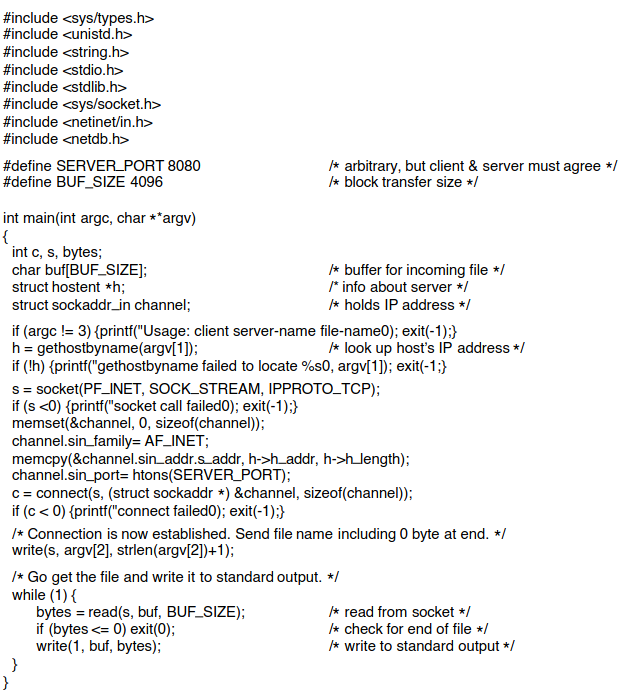
\includegraphics[width=0.85\textwidth]{gambar/socket_client_code}
  \caption{Kode Socket Sisi Klien}
\end{figure}

\begin{figure}[H]
  \centering{}
	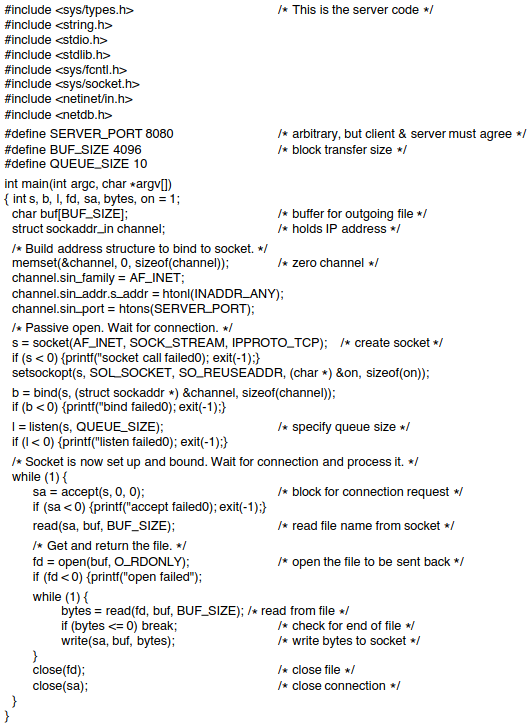
\includegraphics[width=0.85\textwidth]{gambar/socket_server_code}
  \caption{Kode Socket Sisi Server}
\end{figure}

\section{\emph{Bittorrent}}

Awal mula Bittorrent dicetuskan karena masalah ketika klien mengunduh file dari suatu server yang dapat memungkinkan prosesnya melambat. Jika pada satu waktu, banyak klien yang mengunduh. Hal tersebut menyebabkan menurunnya \emph{bandwith} ketika mengunggah file ke setiap klien. Perbedaan kecepatan internet juga menjadi masalah. Dikarenakan proses unduh akan memiliki kecepatan yang lebih tinggi dibanding dengan unggah. Ketika server memiliki kecepatan unggah yang rendah, maka akan menjadi penghambat. Bittorrent menjadi sebuah solusi untuk menyelesaikan permasalahan tersebut.

BitTorrent adalah teknologi atau protokol yang membuat distribusi file, terutama file berukuran besar, lebih mudah dan hemat bandwidth. Hal ini dicapai dengan memanfaatkan kapasitas unggah \emph{peers} yang mendownload file. Peningkatan pengunduh yang cukup signifikan hanya akan menghasilkan sedikit peningkatan beban pada server yang meng-\emph{hosting} file tersebut. \emph{Peers} adalah sekumpulan dari klien yang melakukan proses unduh dan unggah. Jadi, \emph{peer} tidak hanya mendapati hasil unduhan dari server saja, tetapi juga dari \emph{peer} lain yang melakukan proses unggah file. Proses unggah yang dilakukan dalam protokol Bittorrent dengan memotong file menjadi beberapa kepingan yang disebut pieces. Lalu setiap \emph{peer} yang terhubung akan mendapatkan kepingan yang berbeda. Lalu masing - masing \emph{peer} akan bertukar kepingan untuk melengkapi data dari file tersebut, menjadi satu kesatuan file yang utuh. Pada protokol ini, \emph{peer} bertindak melakukan unduh dan unggah.

\subsection{Arsitektur Bittorrent}

Langkah pertama untuk merilis file menggunakan Bittorrent adalah membuat metadata info dari file tersebut. Metadata ini disebut dengan torrent dan ditetapkan dalam file dengan extension `.torrent'. Pada metadata ini, terdapat info yang terdiri dari url dari \emph{tracker}, \emph{filename}, \emph{size} , \emph{path}, dan \emph{hashing information}. Pembuatan torrent dapat dilakukan dengan aplikasi penyedia layanan torrent.

Proses pembuatan torrent baru berawal dari satu komputer yang memiliki file secara utuh. Lalu file tersebut dibuatkan torrentnya, dengan metadata yang diperlukan. Setelah itu komputer tersebut akan melakukan proses unggah kepada \emph{peer} yang ingin mengunduh. Proses tersebut disebut \emph{seeding} dan yang melakukan proses itu disebut \emph{`seeder'}. Sedangkan \emph{peer} lain yang menambahkan torrent tersebut dapat mengunduhnya. \emph{Peer} yang belum memiliki keseluruhan file atau kepingan dari file disebut \emph{`leecher'}. Semakin banyak \emph{peer} yang terhubung, maka proses mengunduh semakin cepat. Sekumpulan \emph{peer} yang membagikan file yang sama disebut \emph{`swarm'}. Setelah \emph{peer} tersebut memiliki file yang utuh, maka dapat sepenuhnya menjadi \emph{seeder}.

Saat membuat file torrent dari file asli, file asli dipotong menjadi kepingan kecil, biasanya berukuran 512 kb atau 256 kb. Kode hash SHA-1 dari setiap kepingan disertakan dalam berkas torrent. Data yang diunduh diverifikasi dengan menghitung kode hash SHA-1 dan membandingkannya dengan kode SHA-1 dari bagian yang sesuai di file torrent. Dengan cara ini data diperiksa untuk kesalahan dan menjamin pengguna bahwa mereka mengunduh data yang benar. Setiap kali sebuah kepingan diunduh dan diverifikasi, \emph{peer} yang mengunduh melaporkan ke \emph{peer} lain di dalam \emph{swarm} tentang kepingan barunya. Kepingan ini sekarang tersedia untuk \emph{peer} lainnya. 

Bittorrent memiliki dua jenis konsep \emph{peer} to \emph{peer}, \emph{centralized tracker} dan \emph{decentralized tracker}. 

\begin{figure}[H]
  \centering{}
	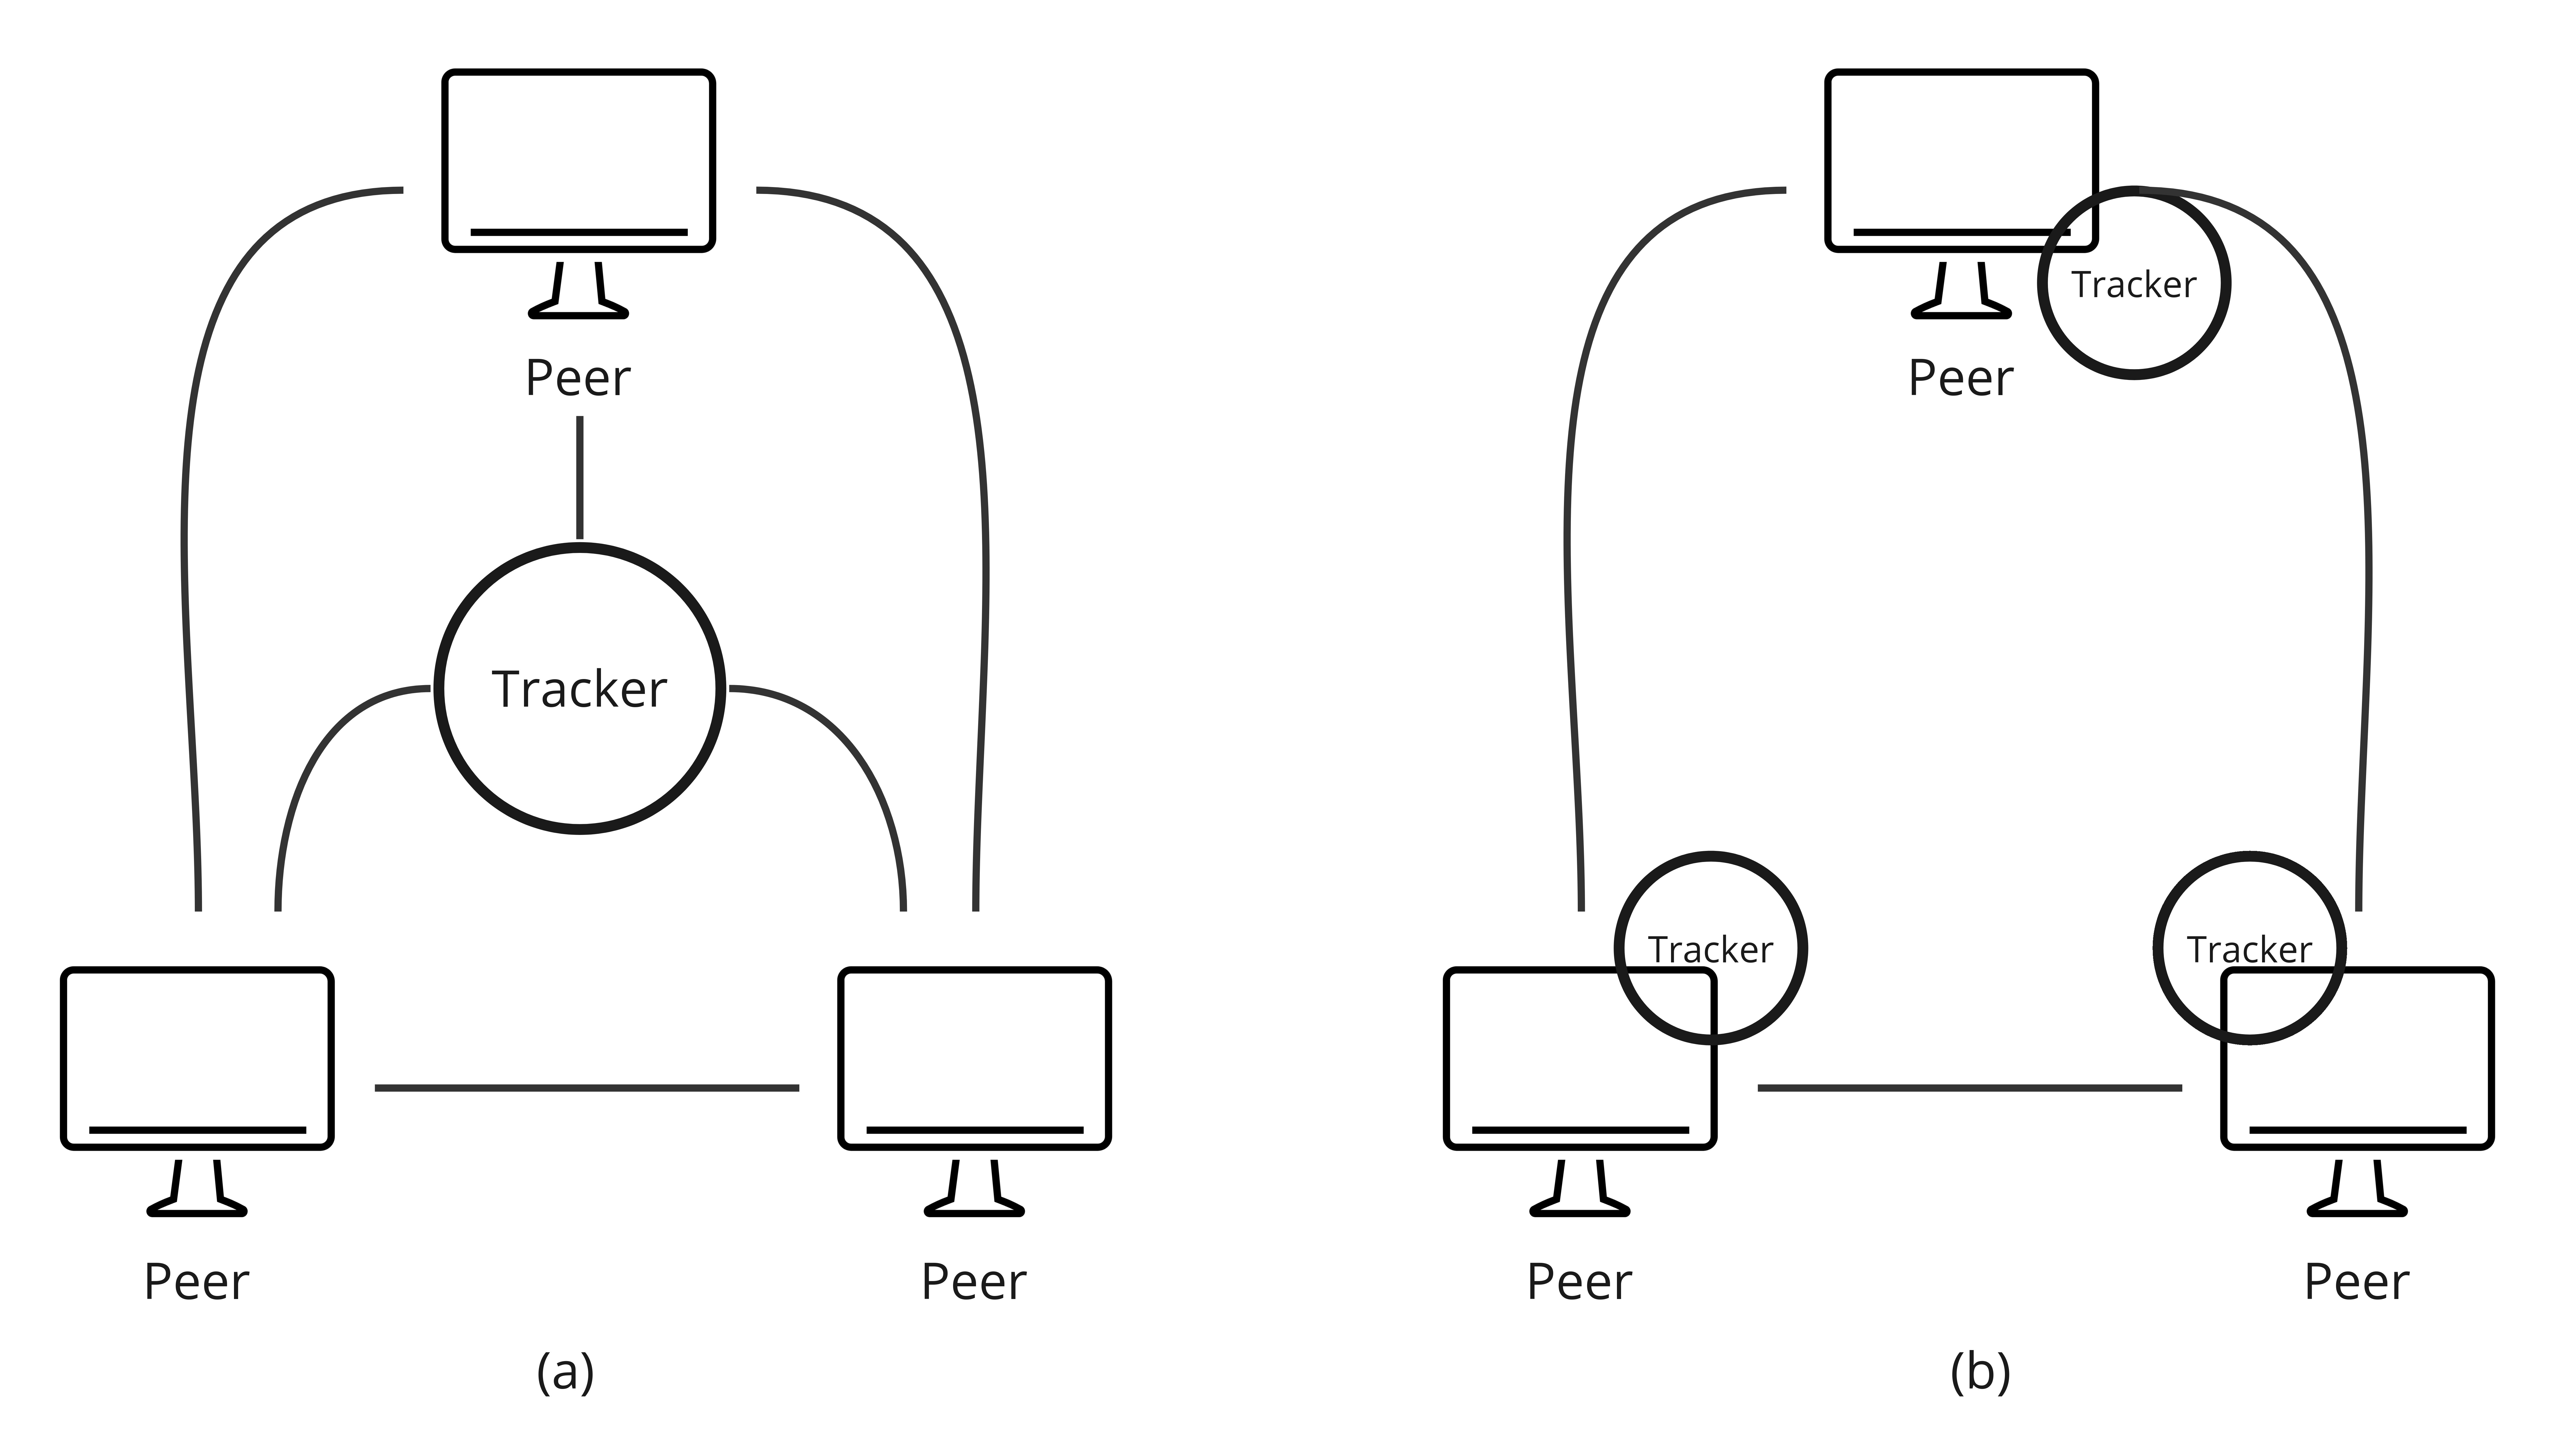
\includegraphics[width=0.85\textwidth]{gambar/bittorrent_arsitektur}
  \caption{(a) \emph{Centralized Tracker}, (b) \emph{Decentralized Tracker}}
\end{figure}

Pada Gambar 2.16 (a) adalah \emph{centralized tracker} dan Gambar 2.16 (b) adalah \emph{decentralized tracker}. \emph{Tracker} atau pelacak menyimpan log peers yang saat ini mengunduh file, dan membantu mereka menemukan satu sama lain. \emph{Tracker} tidak terlibat langsung dalam transfer data dan tidak memiliki salinan file. \emph{Tracker} dan \emph{peer} yang melakukan proses mengunduh bertukar informasi menggunakan protokol sederhana di atas HTTP. Pertama, pengguna memberikan informasi kepada \emph{tracker} mengenai file mana yang diunduh, port yang digunakan, dll. Kemudian \emph{tracker} merespon mengenai daftar \emph{peer} lain yang mengunduh file yang sama dan informasi tentang cara menghubungi mereka.

Pada kedua konsep itu, \emph{tracker} memiliki tugas yang sama. \emph{Decentralized tracker} menjadi sebuah solusi untuk mengatasi kegagalan pada bittorrent dengan \emph{central tracker}. Jika \emph{tracker} tersebut mengalami kegagalan, maka proses distribusi data tidak dapat dilakukan. Dengan adanya \emph{decentralized tracker} menjadi pemecah masalah tersebut. Karena setiap \emph{peer} memiliki trackernya sendiri atau dapat berperilaku sebagai \emph{tracker}. Solusi ini dikembangkan pada Mei 2005 dengan bittorrent versi 4.1 dan berkonsep pada \emph{Distributed Hash Tables} (DHT).

\subsection{\emph{Distributed Hash Tables (DHTs)}}

DHT adalah sistem distribusi \emph{decentralized}. Sistem ini  terdiri dari sekumpulan \emph{node} yang berpartisipasi dan sekumpulan kunci (keys). DHT melakukan fungsi tabel \emph{hash}. Pasangan \emph{key} dan \emph{value} dapat disimpan dan \emph{value} dapat dicari jika \emph{key} yang benar disediakan. Apa yang membedakan DHT dari tabel \emph{hash} biasa adalah penyimpanan dan pencarian didistribusikan di antara \emph{node} (perangkat) dalam jaringan. Semua \emph{node} adalah \emph{peer} yang dapat bergabung dan meninggalkan jaringan secara bebas. DHT membuat jaminan tentang kinerja meskipun terlihat cukup kacau dengan adanya \emph{peer} yang bergabung dan meninggalkan secara acak.

Struktur DHT terdiri dari dua bagian, partisi \emph{keyspace} dan jaringan \emph{overlay}. Partisi \emph{keyspace} menangani partisi \emph{key} di antara \emph{node} dalam jaringan. Jaringan \emph{overlay} menghubungkan \emph{node} dan membiarkan mereka menemukan pemilik \emph{key}. Pada bittorrent menggunakan DHT protokol yang disebut dengan Kademlia.

\subsection{Proses Komunikasi BitTorrent}

Proses komunikasi dan pertukaran data pada protokol bittorrent berlangsung secara \emph{peer to peer}. Mengarah langsung kepada klien, tanpa memerlukan sebuah server. Informasi mengenai \emph{peer} yang terhubung pada jaringan, dengan mendapatkan informasi dari \emph{tracker}. Tetapi \emph{tracker} tidak ikut andil dalam transfer data.
	
Pertama kali \emph{peer} menambahkan torrent file untuk diunduh, saat itu juga \emph{peer} tersebut akan terhubung ke \emph{tracker}, melalui \emph{tracker} url yang tercantum pada torrent file. \emph{Tracker} mendapatkan informasi terkait \emph{peer} yang baru saja terhubung, seperti \emph{IP address} dan \emph{port} bittorrent klien yang digunakan. Jika klien berada pada private IP, maka dengan sendirinya bittorrent akan melakukan \emph{port forwarding}, yang populer dengan menggunakan UPnP (\emph{Universal Plug and Play}). \emph{Port forwarding} berguna agar \emph{peer} tersebut dapat terkoneksi dengan \emph{peer} lain, karena IP dan \emph{port} dari \emph{peer} sudah di-\emph{forward}. Setelah itu, \emph{tracker} memberikan sekumpulan \emph{peer} yang terhubung dengan torrent yang sama. 

\emph{Peer} yang baru terhubung memiliki informasi tersebut untuk meminta \emph{piece} file yang dibutuhkan dengan algoritma dan kebijakan yang ada. Sebelum meminta \emph{piece} file, terlebih dahulu \emph{peer} melakukan \emph{`handshake'} atau proses untuk membuat suatu koneksi dengan \emph{peer} lain yang memiliki \emph{piece}. \emph{Handshake} dilakukan dengan terhubung melalui \emph{IP address} dan \emph{port} dari masing - masing \emph{peer}. Setelah \emph{handshake} berhasil, \emph{peer} tersebut dapat berbagi data.

\section{Algoritma pada Bittorrent}

Di banyak protokol \emph{file sharing peer-to-peer} lainnya, pertukaran file terjadi satu-ke-satu, artinya pengguna sendiri yang memilih rekan lain untuk mengunduh. Konsep BitTorrent adalah dapat mengunduh dari banyak \emph{peer} lainnya secara bersamaan. Ini membutuhkan cara untuk mengetahui \emph{peer} mana yang akan mengunduh dari bagian file yang mana, tujuannya untuk menerima file secara utuh secepat mungkin. Memilih \emph{peer} untuk terhubung adalah masalah dua sisi. Pertama, membutuhkan cara untuk menemukan yang terbaik urutan unduh kepingan file. Kedua, \emph{peer} yang memiliki kepingan yang diinginkan, mungkin tidak mengizinkan \emph{peer} lain mengunduhnya. Strategi untuk \emph{peer} yang tidak mengizinkan \emph{peer} lain mengunduh dari mereka dikenal sebagai \emph{choking}, dan menyangkut \emph{resource allocation}.

\subsection{\emph{Piece Selection}}

Tujuan dari algoritma ini adalah untuk mereplikasi kepingan yang berbeda pada \emph{peer} yang berbeda sesegera mungkin. Ini akan tingkatkan kecepatan pengunduhan, dan juga pastikan semua bagian file ada di suatu tempat di jaringan jika \emph{seeder} utama meninggalkan jaringan. BitTorrent menggunakan TCP dan karenanya penting untuk selalu mentransfer data atau kecepatan transfer akan drop karena mekanisme mulai lambat. Kepingan atau \emph{pieces} tersebut selanjutnya dipecah menjadi sub-kepingan atau sub-\emph{piece},biasanya berukuran sekitar 16kb. Terdapat beberapa kebijakan atau policy yang diterapkan pada bittorrent.

\subsection{\emph{Strict Policy}}

Setelah sub-\emph{piece} diminta, sub-\emph{piece} yang tersisa untuk bagian tertentu itu diminta sebelum sub-\emph{piece} dari bagian lain. Ini membantu mendapatkan bagian utuh dari file secepat mungkin. Jadi setiap \emph{peer} yang terhubung memungkinkan untuk memiliki setiap sub-\emph{piece} yang berbeda dari \emph{peer} utama pemilik file yang utuh.

\subsection{\emph{Rarest First}}

Suatu \emph{peer} memilih \emph{piece} berikutnya untuk diunduh, memilih bagian yang paling sedikit dimiliki oleh \emph{peer} yang berada di dalam satu swarm. Bertujuan agar setiap \emph{piece} tersebar secara merata. Mempercepat proses unduh, karena \emph{piece} tersebut tersebar di \emph{peer} lain. Menjadikan \emph{peer} lain memiliki opsi lain untuk mendapatkan \emph{piece} tersebut. Dengan mengumpulkan \emph{piece} paling langka, akan menjadikan \emph{piece} yang common ditempatkan pada urutan terakhir, karena pasti banyak \emph{peer} yang memiliki \emph{piece} tersebut. Kebijakan ini juga mencegah \emph{piece} yang langka ini hilang. Apabila terjadi kegagalan pada seeder utama dan \emph{piece} yang langka ini belum dimiliki.

\subsection{\emph{Random \emph{Piece} First}}

Ketika \emph{peer} pertama kali terhubung, \emph{peer} tersebut tidak memiliki \emph{piece} apapun untuk diunggah dan dibagikan ke \emph{peer} lain. Oleh karena itu, penting untuk mendapatkan \emph{piece} secepat mungkin dengan cara mengunduh \emph{piece} secara random. Kebijakan ini lebih efisien dibanding rarest first. Jika semua \emph{peer} mengambil \emph{piece} paling langka, maka kecepatan unduh akan berkurang, karena sama - sama menginginkan \emph{piece} yang sama. Jadi, untuk langkah pertama yang dilakukan oleh \emph{peer} ketika terhubung adalah dengan mengambil \emph{piece} secara acak.

\subsection{\emph{Endgame Mode}}

Terkadang \emph{piece} yang diunduh dari \emph{peer} memiliki kecepatan transfer yang lambat. Ini bisa berpotensi menunda penyelesaian unduhan. Untuk mencegah hal ini, bittorent memiliki "endgame mode". Pada prinsip pipelining, yang memastikan bahwa \emph{peer} selalu memiliki sejumlah permintaan (sub-\emph{piece}) tertunda, jumlahnya sering ditetapkan menjadi lima. Ketika semua sub-\emph{piece} pada \emph{peer} kekurangan diminta oleh \emph{peer} lain, permintaan ini disiarkan ke semua \emph{peer}. Ini membantu untuk mendapatkan \emph{piece} terakhir file secepat mungkin. Setelah sub-\emph{piece} tiba, \emph{peer} mengirimkan pesan pembatalan menunjukkan bahwa \emph{peer} tersebut telah memperolehnya dan \emph{peer} lain dapat mengabaikan permintaan tersebut. Beberapa bandwidth tentu saja disia-siakan oleh penyiaran ini, tetapi dalam praktiknya hal ini tidak terlalu banyak karena periode singkat dari mode endgame.

\section{\emph{Resource Allocation Bittorrent}}

Tidak ada alokasi sumber daya terpusat di BitTorrent. Setiap \emph{peer} bertanggung jawab atas memaksimalkan tingkat unduhannya. Seorang \emph{peer}, secara alami, akan mencoba mengunduh dari siapa pun yang mereka bisa. Untuk memutuskan \emph{peer} mana yang akan diunggah, \emph{peer} menggunakan varian dari algoritma `tit-for-tat'. `tit-for-tat' adalah strategi yang berasal dari teori permainan berulang, dan merupakan strategi berbasis kerjasama pada timbal balik. Intinya adalah lakukan pada yang lain seperti yang mereka lakukan.

\subsection{\emph{Choking}}

\emph{Chocking} adalah penolakan sementara untuk mengunggah ke \emph{peer} lain, tetapi \emph{peer} itu masih dapat mengunduh dari \emph{peer} yang ditolak. Prinsipnya unggah ke \emph{peer} yang sudah unggah kepada kita sebelumnya. Tujuannya adalah untuk memiliki beberapa koneksi dua arah kapan saja, dan mencapai `efisiensi Pareto'.
	
\emph{Peer} selalu \emph{unchokes} sejumlah tetap dari \emph{peer} (standarnya adalah empat). Memutuskan \emph{peer} mana yang akan \emph{unchokes} hanya ditentukan oleh tingkat unduh saat ini. Telah dipilih untuk menggunakan 20 detik rata - rata untuk memutuskan ini. Karena penggunaan TCP, tidak diatur untuk \emph{choke} dan \emph{un-choke} juga dengan cepat. Jadi, ini dihitung setiap sepuluh detik.
	
Hasilnya adalah setiap rekan akan mengunggah ke \emph{peer} yang memberikan tingkat unduhan terbaik. Itu sebaliknya; jika tingkat unggahan kita tinggi, lebih banyak \emph{peer} yang memungkinkan untuk kita unduh dari mereka. Ini berarti kita bisa mendapatkan tingkat unduhan yang lebih tinggi jika kita memiliki banyak unggahan. Ini fitur paling penting dari protokol BitTorrent. Ini melarang sejumlah besar "penumpang gratis" atau \emph{`freerider'} yang merupakan \emph{peer} yang hanya mengunduh dan tidak mengizinkan pengunggahan. Agar \emph{peer-to-peer} jaringan berjalan secara efisien, semua peer harus berkontribusi ke jaringan. Pembatasan ini tidak hadir di sebagian besar protokol dan aplikasi \emph{peer-to-peer} lainnya, dan merupakan salah satu alasannya BitTorrent telah menjadi sangat populer.

\subsection{\emph{Optimistic Unchoking}}

\emph{Optimistic Unchoking} adalah variasi dari choking. Setiap beberapa waktu tertentu, \emph{peer} melakukan \emph{optimistic unchoke}. Proses tersebut yang dilakukan \emph{peer}, memilih \emph{peer} lain yang terlihat kurang aktif pada swarm, \emph{peer} tersebut akan disebut sebagai \emph{peer unchoked}. \emph{Peer} yang memilih \emph{peer unchoked} akan mengirimkan \emph{piece} kepadanya. Membuat \emph{peer unchoked} kembali aktif dalam transfer data. Hal ini bertujuan untuk memberikan kesempatan kepada \emph{peer unchoked} untuk meningkatkan koneksi dengan \emph{peer} lain, dan dapat berbagi \emph{piece} dengan \emph{piece} lainnya. Dapat menghindari beberapa \emph{peer} yang dominan dan mengendalikan transfer data secara masif.

\section{\emph{Network Address Translation (NAT)}}

\emph{Network address translation} (NAT) adalah metode pemetaan ruang alamat IP ke yang lain dengan memodifikasi informasi alamat jaringan di header IP paket saat mereka transit melintasi perangkat perutean lalu lintas atau \emph{router}. Teknik ini awalnya digunakan untuk melewati kebutuhan untuk menetapkan alamat baru ke setiap \emph{host} saat jaringan dipindahkan, atau saat penyedia layanan internet diganti, tetapi tidak dapat merutekan ruang alamat jaringan. Ini telah menjadi alat yang populer dan penting dalam melestarikan ruang alamat \emph{global} dalam menghadapi keterbatasan alamat IPv4. Satu alamat IP yang dapat dirutekan internet dari gateway NAT dapat digunakan untuk seluruh jaringan pribadi. Karena NAT memodifikasi informasi alamat IP dalam paket, implementasi NAT dapat bervariasi dalam perilaku spesifiknya dalam berbagai kasus pengalamatan dan pengaruhnya terhadap lalu lintas jaringan.

Perangkat NAT memungkinkan penggunaan alamat IP pribadi pada jaringan pribadi di belakang \emph{router} dengan satu alamat IP publik yang menghadap ke internet. Perangkat jaringan internal berkomunikasi dengan \emph{host} di jaringan eksternal dengan mengubah alamat sumber permintaan keluar ke perangkat NAT dan menyampaikan balasan kembali ke perangkat asal.

\subsection{Klasifikasi NAT}

\emph{Network address} dan \emph{translation port} dapat diimplementasikan dalam beberapa cara. Beberapa aplikasi yang menggunakan informasi alamat IP mungkin perlu menentukan alamat eksternal dari penerjemah alamat jaringan. Ini adalah alamat yang dideteksi oleh \emph{peer} komunikasinya di jaringan eksternal. Selain itu, mungkin perlu untuk memeriksa dan mengkategorikan jenis pemetaan yang digunakan, misalnya bila diinginkan untuk mengatur jalur komunikasi langsung antara dua klien yang keduanya berada di belakang \emph{gateway} NAT yang terpisah. NAT juga diklasifikasikan menjadi empat tipe:

\begin{enumerate}
  \item{\emph{Full-cone NAT}}
  \begin{figure}[H]
    \centering{}
    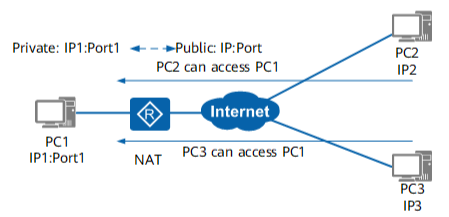
\includegraphics[width=0.85\textwidth]{gambar/full_cone_nat}
    \caption{\emph{Full-cone NAT}}
  \end{figure}

  Semua alamat berasal dari satu internal alamat IP dan \emph{port} yang sama akan dipetakan pada satu eksternal alamat IP dan \emph{port}. Setiap \emph{host} eksternal dapat mengirim paket ke \emph{host} internal, dengan mengirimkan paket ke yang dipetakan alamat eksternal.
  
  \break
  \item{\emph{Address-restricted-cone NAT}}
  \begin{figure}[H]
    \centering{}
    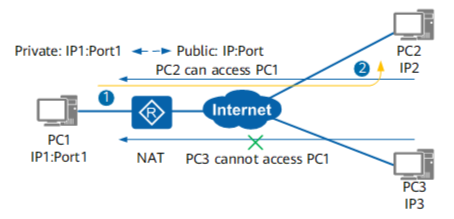
\includegraphics[width=0.85\textwidth]{gambar/address_restricted_cone_nat}
    \caption{\emph{Address-restricted-cone NAT}}
  \end{figure}

  Semua permintaan dari alamat IP internal \emph{port} dipetakan ke yang alamat IP dan \emph{port} eksternal yang sama. Berbeda dari \emph{Full-cone}, eksternal \emph{host} (dengan alamat IP A) dapat mengirim paket ke \emph{host} internal hanya jika \emph{host} internal sebelumnya mengirim paket ke IP alamat A.

  \item{\emph{Port-restricted-cone NAT}}
  \begin{figure}[H]
    \centering{}
    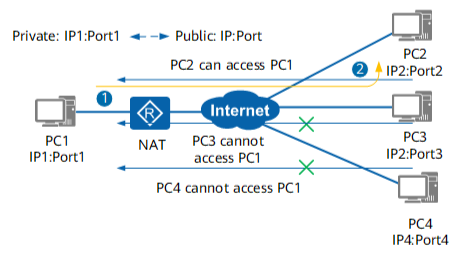
\includegraphics[width=0.85\textwidth]{gambar/port_restricted_cone_nat}
    \caption{\emph{Port-restricted-cone NAT}}
  \end{figure}

  Mirip seperti \emph{Address-restricted-cone}, tetapi pembatasan tersebut mencakup nomor \emph{port}. Secara khusus, \emph{host} eksternal dapat mengirim paket, dengan IP sumber alamat A dan \emph{port} sumber P, ke \emph{host} internal hanya jika \emph{host} internal sebelumnya telah mengirim paket ke alamat IP A dan \emph{port} P.

  \item{\emph{symmetric NAT}}
  \begin{figure}[H]
    \centering{}
    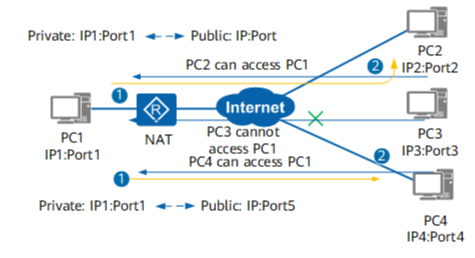
\includegraphics[width=0.85\textwidth]{gambar/symmetric_nat}
    \caption{\emph{Symmetric NAT}}
  \end{figure}

  Semua permintaan dari alamat IP internal dan \emph{port} yang sama, ke alamat IP dan \emph{port} yang spesifik, dipetakan ke alamat IP eksternal dan \emph{port} yang sama. Jika \emph{host} yang sama mengirimkan paket dengan sumber yang sama alamat dan \emph{port}, tetapi ke tujuan yang berbeda, maka akan menggunakan pemetaan yang berbeda. Hanya \emph{host} eksternal yang menerima paket dapat mengirim paket UDP kembali ke \emph{host} internal.
\end{enumerate}

\nocite{liu2021whatisnat}
\nocite{rosenberg2003stun}

\subsection{\emph{NAT Traversal}}

NAT \emph{traversal} adalah teknik jaringan komputer untuk membangun dan menjaga koneksi Protokol internet di seluruh \emph{gateway} yang menerapkan \emph{network address translation} (NAT). Teknik NAT \emph{traversal} diperlukan untuk banyak aplikasi jaringan, seperti berbagi file \emph{peer-to-peer}. Masalah NAT \emph{traversal} muncul ketika \emph{peer} di belakang NAT yang berbeda mencoba untuk berkomunikasi. Salah satu cara untuk mengatasi masalah ini adalah dengan menggunakan \emph{port forwarding}. Cara lain adalah dengan menggunakan berbagai teknik \emph{traversal} NAT. Teknik yang paling populer untuk \emph{traversal} UDP NAT adalah UDP \emph{hole punching}.

\subsection{\emph{UDP Hole Punching}}

UDP \emph{hole punching} membangun konektivitas antara dua \emph{host} yang berkomunikasi melalui satu atau lebih penerjemah alamat jaringan. Biasanya, \emph{host} pihak ketiga di jaringan publik digunakan untuk menetapkan status \emph{port} UDP yang dapat digunakan untuk komunikasi langsung antara \emph{host} yang berkomunikasi. Setelah status \emph{port} berhasil dibuat dan \emph{host} berkomunikasi, status \emph{port} dapat dipertahankan baik oleh lalu lintas komunikasi normal, atau jika tidak ada lagi, dengan paket \emph{keep-alive}, biasanya terdiri dari paket UDP kosong atau paket dengan minimal, non-intrusive konten yang mengganggu.

Salah satu cara untuk melakukan UDP \emph{hole punching} memerlukan \emph{intermediary} atau perantara. Perantara ini disebut sebagai \emph{rendezvous server} atau server pertemuan. Guna dari server pertemuan ini adalah agar masing - masing klien terhubung dan mendapatkan alamat IP dan \emph{port} publik yang diberikan \emph{router} kepada proses komunikasi yang berada di belakang NAT dengan alamat IP dan \emph{port private}. Server pertemuan ini harus berada pada publik IP. Langkah yang terjadi ketika dua klien ingin melakukan komunikasi, yang mana kedua klien tersebut berada di belakang NAT adalah dengan mengirim udp packet ke server pertemuan. Lalu server akan mendapatkan alamat IP dan \emph{port} address publik dari klien tersebut. Lalu melakukan pertukaran alamat IP dan \emph{port} publik dari klien A kepada klien B, dan sebaliknya. Setelah mendapatkan masing - masing alamat IP dan \emph{port} dari masing - masing klien. Klien A dapat mengirim packet data ke klien B melalui alamat IP dan \emph{port} publiknya, dan sebaliknya. Setelah itu, kedua klien terhubung, walaupun server pertemuan dimatikan atau koneksi dari server terputus, kedua klien tersebut tetap dapat terhubung dan berkomunikasi, karena telah membuat `lubang' pada NAT.

\nocite{ford2005peer}

\begin{figure}[H]
  \centering{}
  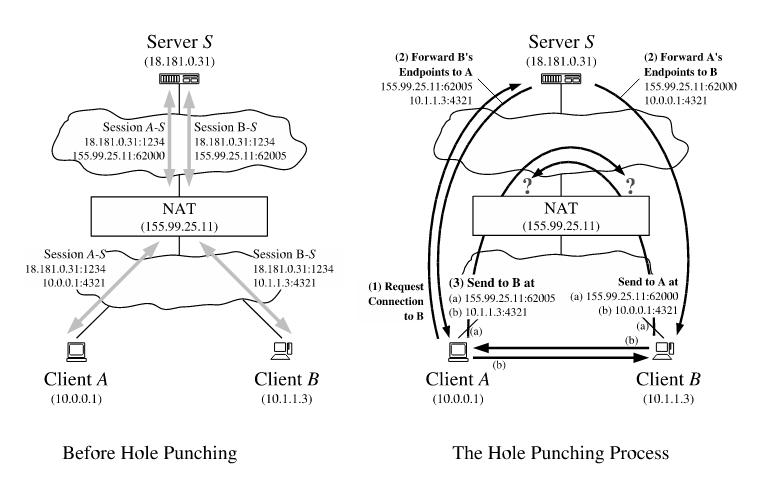
\includegraphics[width=1\textwidth]{gambar/hole_punching_behind_same_nat_1}
  \caption{Sebelum \emph{Hole Punching} di Belakang Satu NAT yang Sama.}
\end{figure}

\begin{figure}[H]
  \centering{}
  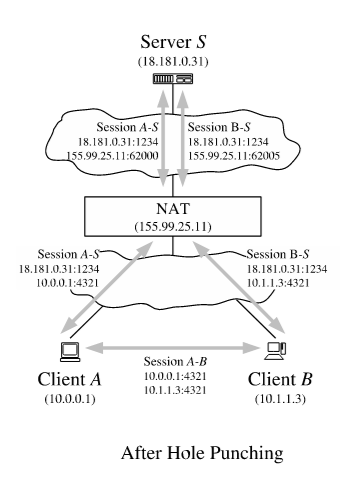
\includegraphics[width=0.5\textwidth]{gambar/hole_punching_behind_same_nat_2}
  \caption{Setelah \emph{Hole Punching} di Belakang Satu NAT yang Sama.}
\end{figure}


\begin{figure}[H]
  \centering{}
  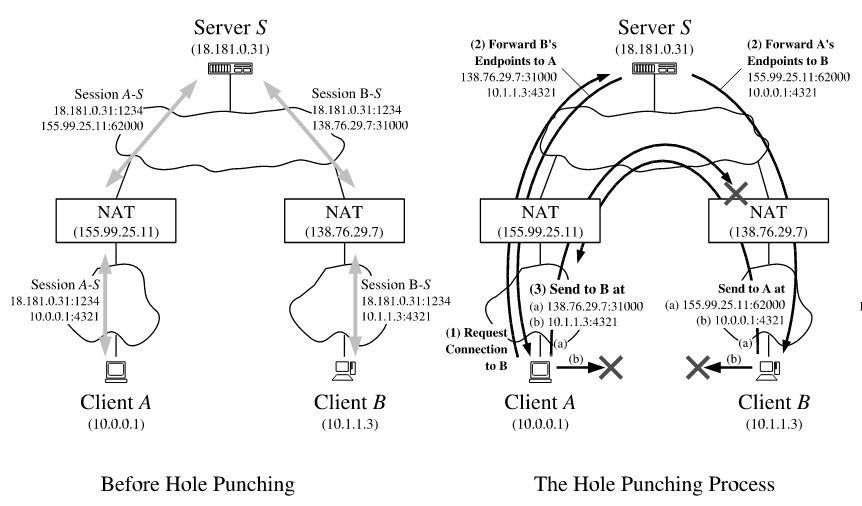
\includegraphics[width=1\textwidth]{gambar/hole_punching_behind_different_nat_1}
  \caption{Sebelum \emph{Hole Punching} di Belakang NAT yang Berbeda.}
\end{figure}

\begin{figure}[H]
  \centering{}
  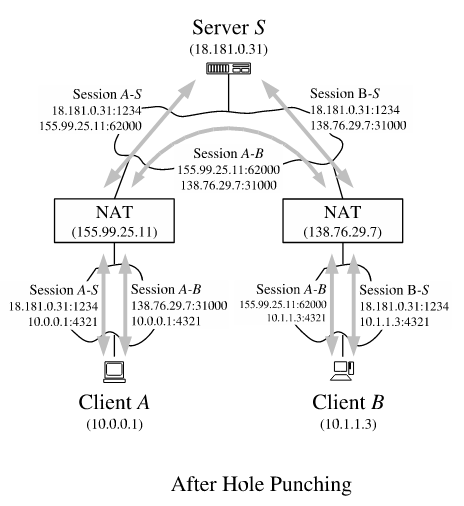
\includegraphics[width=0.5\textwidth]{gambar/hole_punching_behind_different_nat_2}
  \caption{Setelah \emph{Hole Punching} di Belakang NAT yang Berbeda.}
\end{figure}

\begin{figure}[H]
  \centering{}
  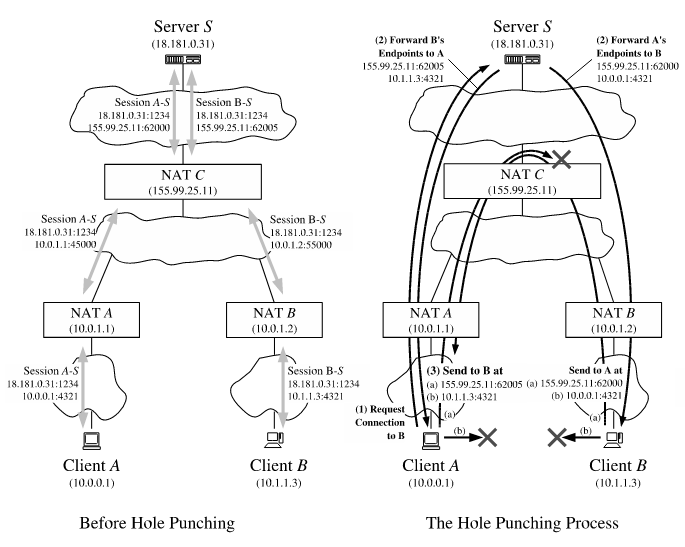
\includegraphics[width=0.8\textwidth]{gambar/hole_punching_behind_different_level_nat_1}
  \caption{Sebelum \emph{Hole Punching} di Belakang Berbagai Level NAT.}
\end{figure}

\begin{figure}[H]
  \centering{}
  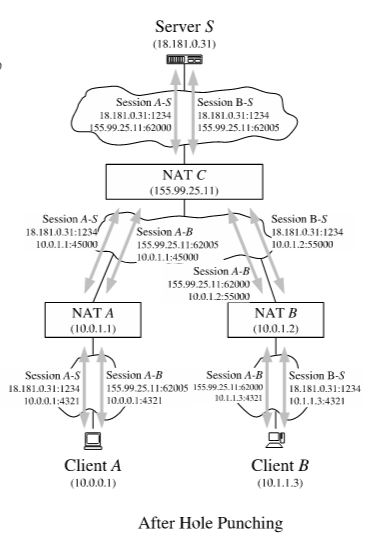
\includegraphics[width=0.5\textwidth]{gambar/hole_punching_behind_different_level_nat_2}
  \caption{Setelah \emph{Hole Punching} di Belakang Berbagai Level NAT.}
\end{figure}

\subsection{\emph{Timeouts}}

NAT melakukan pemetaan alamat eksternal dan \emph{port} untuk setiap klien yang ingin melakukan koneksi ke internet. Banyak perangkat NAT mematikan pemetaan tersebut jika tidak ada aktivitas yang terjadi dalam rentang waktu tertentu, beberapa NAT memiliki \emph{timeouts} yang pendek sekitar 20 detik. Yang akan bervariasi tergantung dari perangkat dan konfigurasinya. Akan menjadi sebuah masalah jika pemetaan NAT untuk komunikasi antara klien berubah. Cara untuk mengatasi hal ini adalah dengan mengirim paket \emph{keep alive} setiap beberapa rentang waktu. Untuk menjaga serta memastikan koneksi tetap terhubung antara klien. Paket \emph{keep alive} biasanya berupa paket dengan ukuran kecil.

Tetapi, banyak NAT mengasosiasikan \emph{idle timer} UDP dengan sesi UDP individual, jadi mengirim \emph{keep-alive} pada satu sesi tidak akan membuat sesi lain tetap aktif meskipun semua sesi berasal dari titik akhir \emph{private} yang sama. Alih-alih mengirim \emph{keep-alive} di berbagai sesi P2P, aplikasi dapat menghindari lalu lintas \emph{keep-alive} yang berlebihan dengan mendeteksi kapan sesi UDP tidak lagi berfungsi, dan menjalankan kembali prosedur \emph{hole punching} lagi \emph{`on demand'}.

Koneksi TCP dapat tetap dalam fase yang ditetapkan tanpa batas waktu bertukar paket apapun. Beberapa host akhir dapat dikonfigurasi untuk mengirim paket \emph{keep-alive} pada koneksi yang \emph{idle}; secara \emph{default}, paket \emph{keep-alive} dikirim setiap 2 jam jika diaktifkan. Akibatnya, NAT yang menunggu lebih dari 2 jam dapat mendeteksi koneksi \emph{idle} dengan paket \emph{keep-alive} dikirim secara \emph{default}. Koneksi TCP dalam fase \emph{partially open} atau \emph{closing}, di sisi lain, bisa \emph{idle} paling lama 4 menit sambil menunggu paket dalam pengiriman yang akan dikirimkan.

\section{\emph{Distributed Web Crawler Architecture}}

\emph{Web crawler} dikembangkan dari awal dikenalkannya web. Beberapa generasi pertama \emph{web crawler} pada awal tahun 90-an yaitu: \emph{World Wide Worm}, \emph{RBSE Spider}, \emph{MOMspider}, dan \emph{WebCrawler}. Berawal dari generasi ini yang memiliki kontribusi besar terhadap algoritma utama dan \emph{design issues} dari \emph{web crawler}. Beberapa komersial \emph{search engine} memiliki dan mengembangkan \emph{crawler}-nya masing - masing. Seiring berkembangnya \emph{crawler}, sampai pada generasi sekarang, yang mana diharapkan mampu mengunduh miliaran halaman web dengan cepat. Dan semua itu tidak ada yang tersedia secara gratis dan \emph{open source}. BUbiNG adalah \emph{open source} \emph{crawler} pertama yang didesain untuk menjadi \emph{crawler} yang \emph{fast}, \emph{scalable}, dan \emph{runnable} di perangkat keras secara luas. Arsitektur dari \emph{web crawler} BUbiNG akan menjadi referensi dari penelitian ini untuk menentukan distribusinya.

\nocite{boldi2018bubing}

\begin{figure}[H]
  \centering{}
  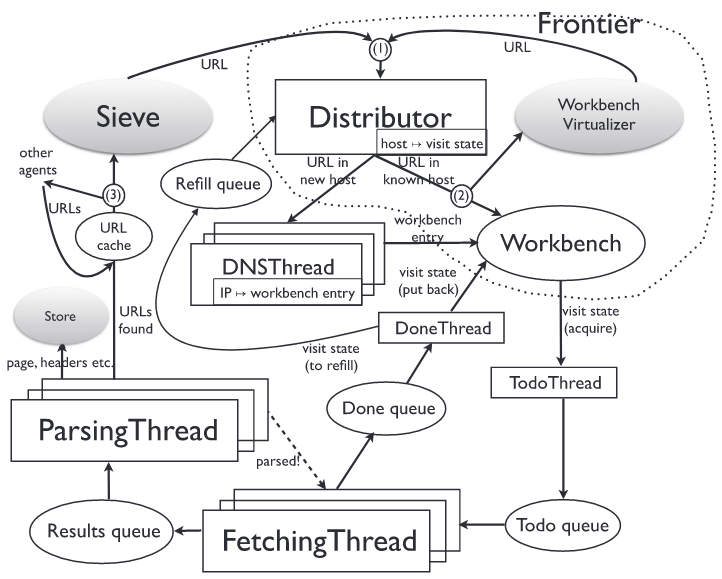
\includegraphics[width=0.85\textwidth]{gambar/bubing_architecture}
  \caption{Arsitektur BUbiNG}
\end{figure}

Proses \emph{crawling} berawal dari \emph{fetching thread}, pada tahap ini menghabiskan banyak waktu untuk menunggu data jaringan. Biasanya mengalokasikan \emph{parsing threads} sebanyak jumlah \emph{core} yang tersedia, karena aktivitasnya sebagian besar terikat CPU. Saat \emph{parsing threads} menemukan URL baru, dimasukkan ke \emph{sieve} yang melacak URL yang telah ditemukan. \emph{Sieve} adalah struktur data yang mirip dengan antrean dengan memori: setiap elemen yang di-\emph{queue} (masuk dalam antrean) akan di-\emph{dequeued} (dikeluarkan dari antrean) di lain waktu, dengan jaminan bahwa suatu elemen yang diantrekan beberapa kali akan di-\emph{dequeued} sekali saja. Dengan kata lain, \emph{sieve} bertugas untuk menyaring URL yang ditemukan. URL ditambahkan ke \emph{sieve} saat ditemukan dengan \emph{parsing}. URL yang berada di-\emph{sieve} sudah siap untuk dikunjungi dan akan diatur oleh \emph{frontier}. \emph{Frontier} dapat disebut sebagai kumpulan URL yang sudah ditemukan, tetapi belum di-\emph{crawl}. Pada \emph{frontier}, struktur data terpenting pada adalah \emph{workbench}. Karena pada tahap tersebut, akan mengetahui \emph{visit state} setiap \emph{host} atau perangkat yang melakukan \emph{crawling}. Informasi ini akan dikumpulkan untuk nantinya didistribusikan kepada perangkat lain yang menjalankan \emph{crawler}. Setelah itu, URL yang didapatkan akan disaring (agar tidak ada duplikasi) dan kembali ditempatkan di \emph{workbench}.

Komponen yang aktif pada \emph{frontier} adalah \emph{distributor}. Tugas dari \emph{distributor} adalah untuk mengeluarkan URL dari antrean yang berasal dari \emph{sieve}. Melakukan pengecekan terhadap \emph{visit state} dari masing - masing \emph{host}, apakah sudah dikunjungi oleh \emph{host} tersebut. Jika belum, maka akan membuat \emph{visit state} yang baru atau mengantrekan URL ke yang sudah \emph{visit state} yang sudah ada. Jika \emph{visit state} yang baru diperlukan, diteruskan ke kumpulan DNS threads yang melakukan DNS resolution dan kemudian memindahkan \emph{visit state} ke \emph{workbench}.

\subsection{\emph{Workbench}}

URL yang terkait dengan \emph{host} tertentu disimpan dalam struktur yang disebut \emph{visit state}, berisi antrean FIFO (\emph{First In First Out}) dari URL berikutnya yang akan di-\emph{crawl} untuk \emph{host} tersebut bersama dengan \emph{next-fetch field} yang menentukan saat pertama URL dari antrean dapat diunduh, menurut ke konfigurasi politenesss setiap \emph{host}. \emph{Visit state} hanya menyimpan \emph{byte-array} representasi jalur dan kueri URL: pendekatan ini secara signifikan mengurangi pembuatan objek dan menyediakan bentuk kompresi sederhana dengan penghilangan awalan atau \emph{prefix omission}.

\begin{figure}[H]
  \centering{}
  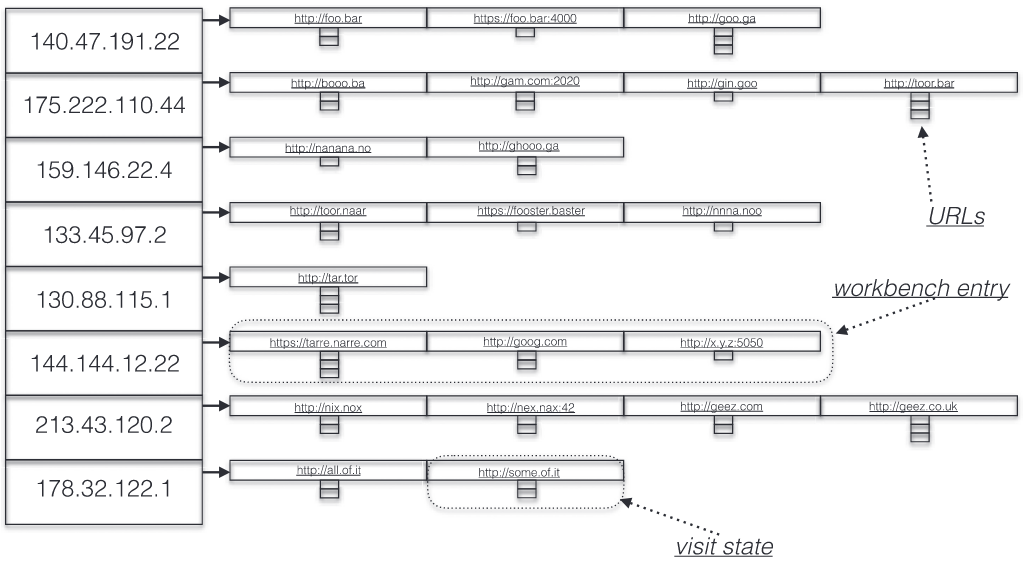
\includegraphics[width=1\textwidth]{gambar/bubing_workbench}
  \caption{BUbiNG \emph{Workbench}}
\end{figure}

\emph{Visit state} selanjutnya dikelompokkan ke dalam entri \emph{workbench} berdasarkan alamat IP mereka; setiap kali URL pertama untuk \emph{host} tertentu ditemukan, \emph{visit state} baru dibuat, lalu alamat IP ditentukan (oleh salah satu \emph{DNS threads}): \emph{visit state} baru dimasukkan ke dalam entri \emph{workbench} baru (jika tidak ada \emph{host} yang diketahui dikaitkan dengan alamat IP itu) atau yang sudah ada. \emph{Workbench} bertindak sebagai menunda antrian (\emph{delay queue}): operasi untuk mengeluarkan dari antrian menunggu, jika perlu, sampai \emph{host} siap untuk dikunjungi. Pada saat itu, entri teratas dihapus dari \emph{workbench} dan \emph{visit state} teratas dihapus dari entri teratas. Kedua penghapusan terjadi dalam waktu logaritmik (dalam jumlah \emph{visit state}).

Akses ke \emph{workbench} terhimpit di antara dua antrean \emph{lock-free} (pendekatan ini sangat berguna untuk menghindari akses langsung ke struktur data yang disinkronkan dengan waktu modifikasi logaritmik, seperti prioritas antrian, sebagai pertentangan antara \emph{fetching thread} bisa menjadi sangat signifikan): \emph{to-do queue} dan \emph{done queue}. Antrian tersebut dikelola oleh dua \emph{thread} prioritas: to-do \emph{thread} mengekstrak \emph{visit state} yang \emph{host}-nya dapat dikunjungi tanpa melanggar batasan politeness dan memindahkannya ke \emph{to-do queue}, di mana akan diambil oleh \emph{fetching thread}; di sisi lain, done thread mengambil \emph{visit state} setelah digunakan oleh \emph{fetching thread} dan mengembalikannya ke \emph{workbench}.
	
Tujuan dari pengaturan ini adalah untuk menghindari pertentangan oleh ribuan \emph{threads} pada struktur yang relatif lambat (karena mengekstraksi dan memasukkan elemen di \emph{workbench} membutuhkan waktu logaritmik dalam jumlah \emph{host}). Membuat jumlah \emph{visit state} yang siap untuk diunduh mudah diukur: ini hanya ukuran antrean tugas. Sisi negatifnya adalah pada prinsipnya menggunakan penundaan politeness per-\emph{host} atau per-IP yang dapat menyebabkan urutan \emph{to-do queue} tidak mencerminkan prioritas sebenarnya dari \emph{visit state} yang terkandung di dalamnya; fenomena ini mungkin mendorong urutan global visit lebih jauh dari breath-first visit.
	
\emph{Workbench virtualizer} mempertahankan pemetaan pada disk dari \emph{host} ke FIFO antrian \emph{virtual} URL. Secara konseptual, semua URL yang telah diekstraksi dari \emph{sieve} tetapi belum diambil akan diantrekan di \emph{visit state} \emph{workbench} tempatnya berada, dalam urutan yang tepat saat keluar \emph{sieve}. Karena, bertujuan melakukan \emph{crawling} dengan jumlah memori yang konstan jumlah URL yang ditemukan, bagian dari antrian harus ditulis di disk. Setiap antrian \emph{virtual} berisi sebagian kecil URL dari setiap \emph{visit state}, sedemikian rupa sehingga keseluruhan urutan URL sesuai, per-\emph{host}, berdasar breadth-first yang asli.

\subsection{\emph{Distributor}}

\emph{Distributor} adalah \emph{high-priority} thread yang mengatur pergerakan URL keluar dari \emph{sieve} dan memuat URL dari antrian \emph{virtual} ke \emph{workbench} seperlunya. Saat \emph{crawling} berlangsung, URL terakumulasi dalam \emph{visit state} dengan kecepatan berbeda, baik karena \emph{host} memiliki daya tanggap koneksi yang berbeda dan karena situs web memiliki ukuran dan faktor percabangan yang berbeda. Selain itu, \emph{workbench} memiliki ukuran batas yang dapat dikonfigurasi agar tidak dapat melampaui batas jumlah ukurannya. Jumlah memori utama yang ditempati tidak dapat bertambah tanpa batas dalam jumlah URL yang ditemukan, tetapi hanya dalam jumlah \emph{host} yang ditemukan. Dengan demikian, mengisi \emph{workbench} secara terus - menerus dengan URL yang keluar dari \emph{sieve} akan segera menghasilkan \emph{workbench} yang hanya berisi URL milik sejumlah \emph{host}. 

Bagian depan (front) \emph{crawling}, pada waktu tertentu, adalah jumlah status kunjungan yang siap untuk diunduh. Ukuran front menentukan \emph{throughput} atau \emph{bandwidth} keseluruhan \emph{crawler}, jumlah \emph{host} berbeda yang sedang dikunjungi adalah yang terpenting untuk menentukan seberapa cepat atau lambat \emph{crawling} akan dilakukan.
	
Salah satu dari dua kekuatan yang menggerakkan \emph{distributor} adalah \emph{front} harus selalu cukup besar sehingga tidak ada \emph{fetching thread} yang harus menunggu. Untuk mencapai tujuan ini, \emph{distributor} diperbesar secara dinamis sesuai ukuran \emph{front} yang dibutuhkan, yang merupakan perkiraan jumlah \emph{host} yang harus dikunjungi secara paralel untuk membuat semua \emph{fetching thread} sibuk: setiap kali \emph{fetching thread} harus menunggu, meskipun demikian ukuran \emph{front} saat ini lebih besar dari ukuran \emph{front} yang dibutuhkan saat ini, yang terakhir ditingkatkan. Setelah fase \emph{warm-up}, ukuran \emph{front} yang diperlukan distabilkan ke nilai yang bergantung pada jenis \emph{host} yang dikunjungi dan pada jumlah sumber daya yang tersedia. Pada saat itu, tidak mungkin untuk memiliki \emph{crawl} lebih cepat mengingat sumber daya yang tersedia, karena semua \emph{fetching thread} terus mengunduh data. Meningkatkan jumlah \emph{fetching thread}, tentu saja, dapat menyebabkan peningkatan ukuran \emph{front} yang dibutuhkan.

\begin{figure}[H]
  \centering{}
  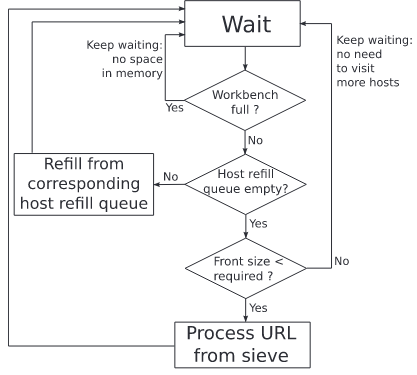
\includegraphics[width=0.6\textwidth]{gambar/bubing_distributor}
  \caption{BUbiNG \emph{Distributor}}
\end{figure}

Kekuatan kedua yang menggerakkan \emph{distributor} adalah persyaratan yang dimiripkan dengan pendekatan \emph{breadth-first visit}. Dengan catatan, kekuatan ini bekerja berlawanan arah dengan memperbesar ukuran \emph{front} URL yang sudah ada dalam \emph{visit state} yang seharusnya, pada prinsipnya, URL akan dikunjungi jika sudah berada pada \emph{sieve}, tetapi memperbesar \emph{front} memerlukan lebih banyak URL yang dikeluarkan dari antrean \emph{sieve} untuk menemukan \emph{host} baru.

\emph{Distributor} bertanggung jawab untuk mengisi \emph{workbench} dengan URL yang akan datang, yang keluar dari \emph{sieve} atau virtual queue. Hak istimewa \emph{distributor} untuk mengisi ulang antreanf \emph{workbench} menggunakan URL dari \emph{virtualizer} (lingkaran bernomor (1) pada Gambar 2.27) karena ini membuat kunjungan lebih dekat ke \emph{breadth-first}. Nafmun, jika tidak ada isi ulang yang harus dilakukan dan \emph{front} tidak cukup besar, \emph{distributor} akan membaca dari \emph{sieve}, berharap menemukan \emph{host} baru untuk membuat \emph{front} lebih besar.

Saat \emph{distributor} membaca URL dari \emph{sieve}, URL tersebut dapat diletakkan di \emph{workbench} (lingkaran bernomor (2) pada Gambar 2.27) atau ditulis dalam antrian virtual, tergantung ada tidaknya sudah URL pada disk untuk \emph{host} yang sama, dan jumlah URL per alamat IP yang seharusnya di \emph{workbench} agar tetap penuh, tetapi tidak \emph{overflowing}, bila \emph{front} sesuai dengan ukuran yang dibutuhkan.


%!TEX root = ./template-skripsi.tex
%-------------------------------------------------------------------------------
%                     BAB III
%               			PEMBAHASAN
%-------------------------------------------------------------------------------

\chapter{METODOLOGI PENELITIAN}

\section{Tahapan Penelitian}

\begin{figure}[H]
  \centering{}
	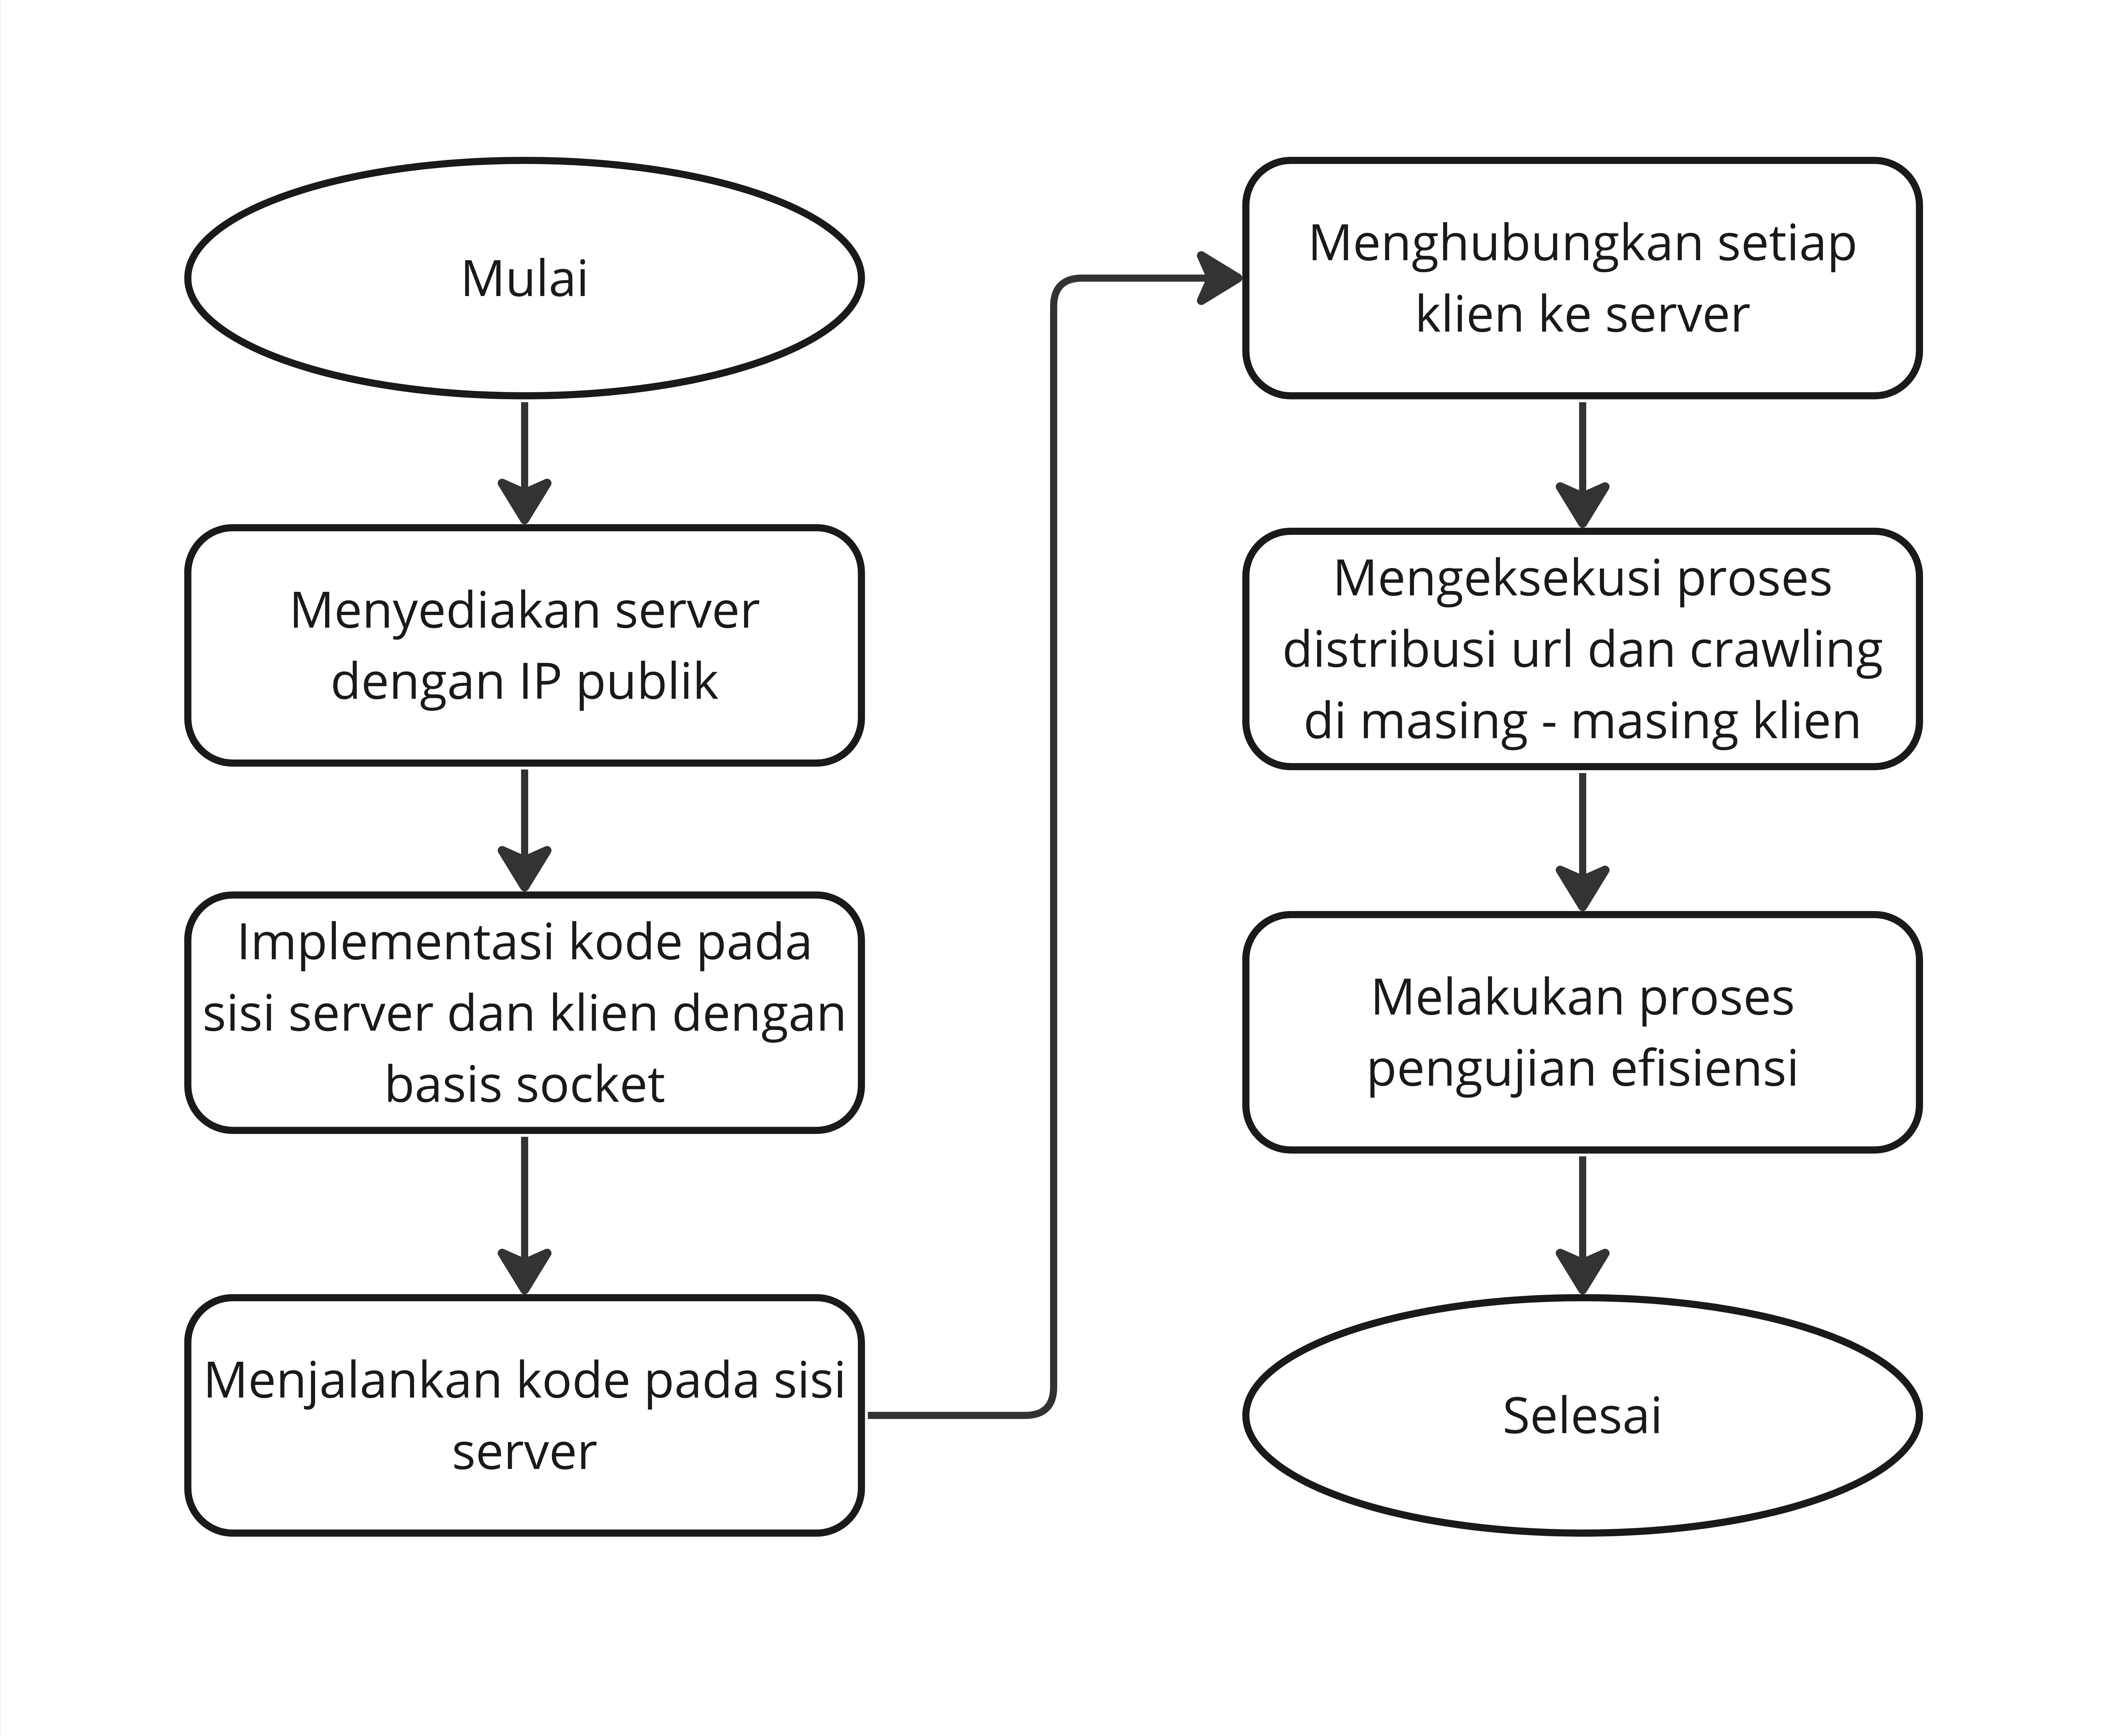
\includegraphics[width=0.6\textwidth]{gambar/flowchart_tahapan_penelitian_crawler_terdistribusi}
  \caption{\emph{Flowchart} Tahapan Penelitian Crawler Terdistribusi}
\end{figure}

Socket berperan penting dalam proses distribusi \emph{url} untuk melakukan crawling pada setiap klien. Karena socket sebagai pokok transportasi url dari satu perangkat ke perangkat yang lain melalui media internet.

Kode program crawler yang ada saat ini hanya menerima masukan url dari perangkat yang menjalankan crawler tersebut. Sedangkan, pada penelitian ini url yang diterima didapatkan dari pembagian dari perangkat lain. Menjadikan klien yang terhubung dapat menjalankan crawling secara bersamaan dan tidak melakukan crawling dengan url yang sama. Jadi tidak ada duplikasi data dari setiap kliennya.

\section{Arsitektur \emph{Crawler} Terdistribusi}

Sistem yang akan dibuat pada penelitian ini adalah pengembangan \emph{crawler} menjadi secara terdistribusi yang dapat berjalan atau melakukan \emph{crawling} pada banyak perangkat sekaligus secara terkontrol. Pengembangan ini menggunakan koneksi socket untuk komunikasi. Gambaran awal arsitektur ini adalah \emph{master-slave}. \emph{Master} bertugas untuk mengelola semua \emph{slave} yang tersedia, melakukan \emph{write operation} ke dalam database, dan membagi serta menyeimbangkan tugas ke masing - masing \emph{slave}. Sedangkan \emph{slave} bertugas untuk melakukan \emph{crawling} dari url yang diberikan oleh \emph{master} dan akan mengembalikan data hasil \emph{crawling} kembali ke \emph{master} untuk dimasukkan ke database, lalu menyeimbangkan kembali url untuk di-\emph{crawling}.

\begin{figure}[H]
  \centering{}
	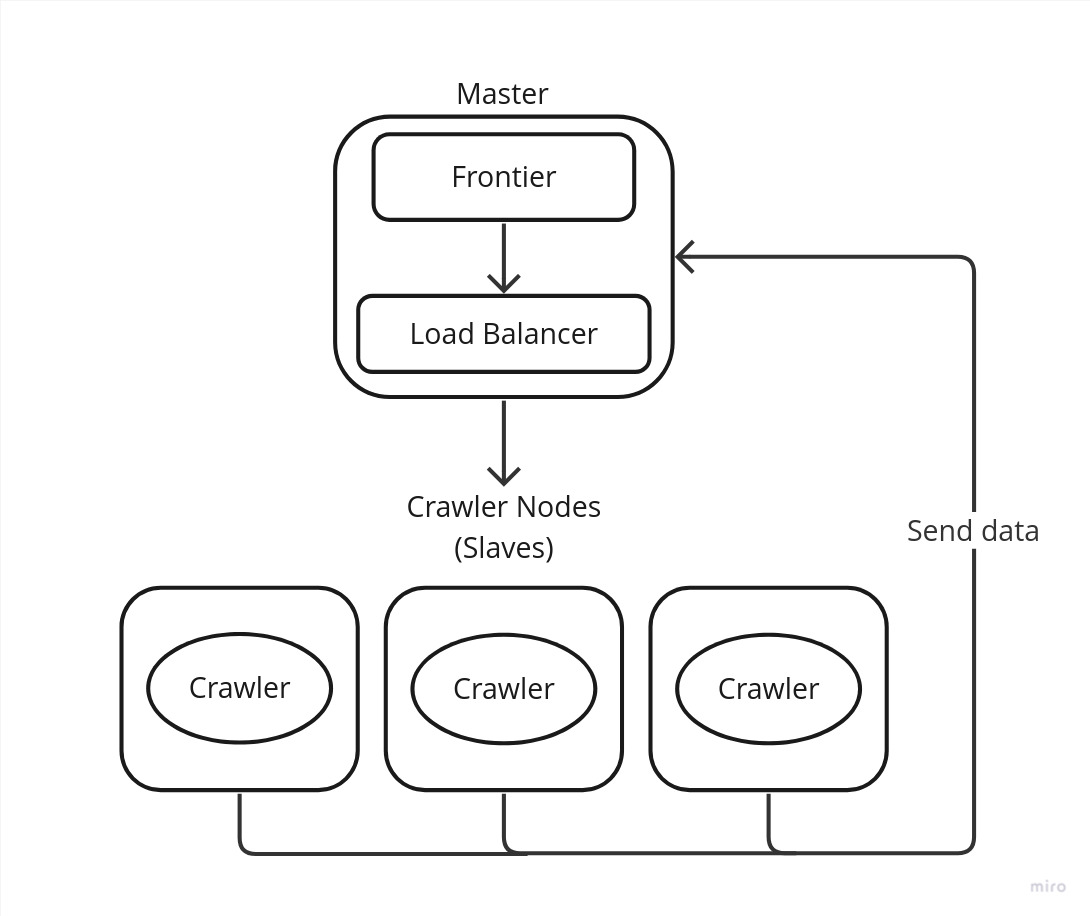
\includegraphics[width=0.6\textwidth]{gambar/crawler_master_slave}
  \caption{Arsitektur \emph{Crawler Master-Slave}}
\end{figure}

\begin{enumerate}
  \item{\emph{Frontier} adalah antrian dari sekumpulan url yang belum dikunjungi dan sudah dikunjungi oleh \emph{crawler}. Url yang terdapat pada \emph{Frontier} sudah terkurasi agar tidak ada url yang terduplikat, guna menghindari melakukan \emph{crawling} pada halaman web yang sama. Kemudian \emph{crawler} akan menerima url dari \emph{frontier} dan melakukan \emph{crawling} pada halaman dari url tersebut.}

  \item{Load balancer bertugas sebagai scheduler untuk mengatur urutan antrian dari url yang akan didistribusikan kepada \emph{crawler}. Mendistribusikan url ke setiap \emph{crawler nodes} agar setiap \emph{crawler} memiliki beban kerja yang seimbang. \emph{Load balancer} memiliki sekumpulan antrian url dari masing - masing \emph{crawler}.}

  \item{\emph{Crawler nodes} adalah perangkat yang akan melakukan \emph{crawler}, url untuk melakukan \emph{crawling} didapatkan dari \emph{frontier} dan hasil dari \emph{crawling} disimpan pada database.}
\end{enumerate}

Berdasarkan arsitektur pada Gambar 3.2, terdapat beberapa pengembangan pada tahapan komunikasi antara \emph{slave} atau klien atau \emph{peer}. Proses komunikasi dilakukan secara langsung antara \emph{peer}, disebut sebagai \emph{peer-to-peer}. Karena komunikasi ini terjadi antara \emph{peer} yang memiliki \emph{private} IP dapat saling berkomunikasi. 

\begin{figure}[H]
  \centering{}
	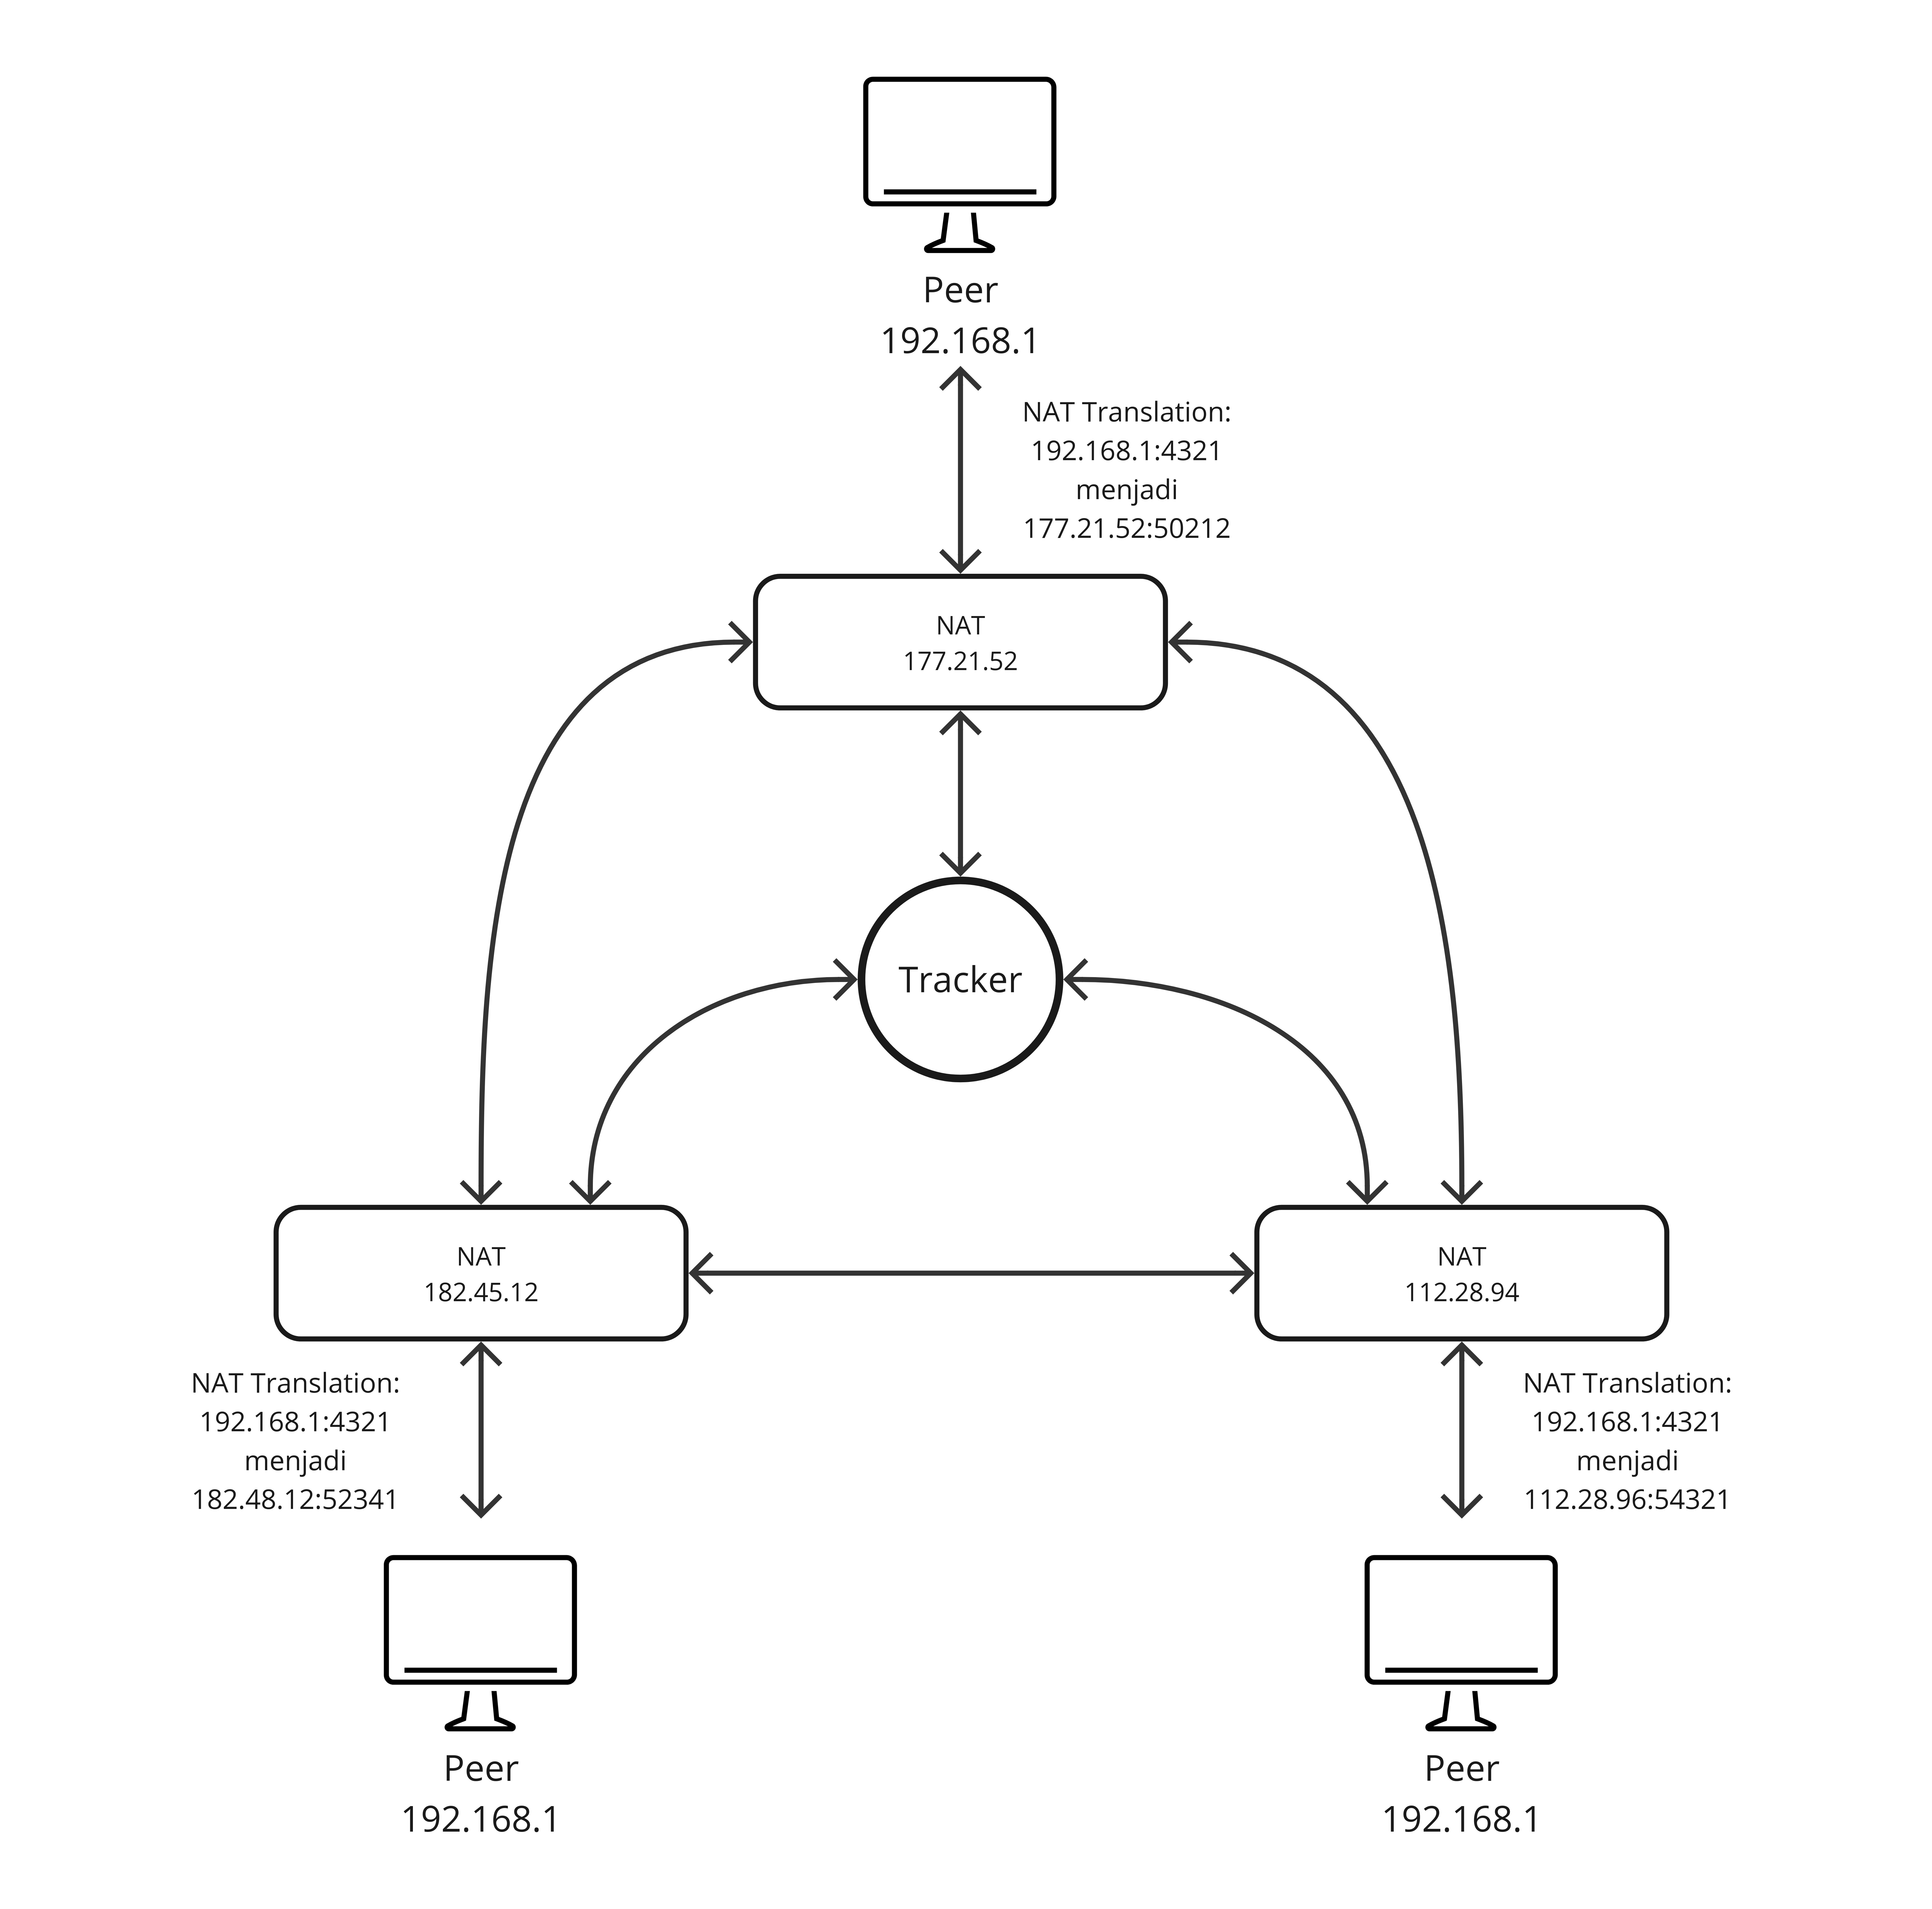
\includegraphics[width=0.6\textwidth]{gambar/peer_to_peer_through_nat}
  \caption{Arsitektur \emph{Crawler Peer to Peer} Melalui NAT}
\end{figure}

\begin{enumerate}
  \item{\emph{Tracker} atau \emph{master} bertugas untuk mengetahui eksternal atau publik IP address dan port dari masing - masing \emph{peer} yang terhubung. \emph{Tracker} adalah sebuah server yang memiliki publik IP. Setelah mengetahui eksternal IP address dan port setiap \emph{peer}, maka \emph{peer} dapat terhubung dengan satu sama lain. Mengoleksi kumpulan \emph{peer} yang terhubung. Setup initial url untuk \emph{crawling}. Melakukan broadcast secara berkala untuk update \emph{peer} yang terhubung dan keluar dari swarm.} 

  \item{\emph{Peer} dapat disebut klien. Setiap \emph{peer} memiliki duplikasi dari kumpulan \emph{peer} yang terhubung dengan \emph{tracker}. Melakukan proses \emph{crawling}. Mengoleksi sekumpulan url untuk di-\emph{crawl}. Mengambil bagian url yang akan di-\emph{crawl} untuk setiap \emph{peer}, saat mengambil url juga mengeluarkannya dari sekumpulan url, sekali mengambil url langsung cukup banyak, bergantung dengan jumlah \emph{peer} yang terhubung, baru di-broadcast kepada semua \emph{peer} yang terhubung atau melalui perantara \emph{tracker} mengenai sekumpulan url yang baru. Minimal menyisakan url lebih banyak dari jumlah \emph{peer} yang terhubung. Agar semua \emph{peer} mendapatkan bagian url yang seimbang. Memasukkan data hasil \emph{crawling} ke database.}
\end{enumerate}

\section{Proses Komunikasi \emph{Peer-to-peer}}

Proses komunikasi menggunakan metode UDP \emph{hole punching}, dengan membuat `lubang' pada NAT, agar antara \emph{peer} dapat saling terhubung antara satu sama lain melalui `lubang' tersebut. Menggunakan socket protokol untuk mengirim packet kepada \emph{tracker} untuk mengetahui publik IP address dari \emph{peer} yang mengirim packet tersebut. Karena \emph{peer} berada di belakang NAT atau router. Jadi IP address dan portnya akan diwakilkan oleh publik IP address dan port dari NAT. Pentingnya untuk mengetahui publik IP address dan portnya, agar \emph{peer} lain dapat terhubung melalui publik IP address dan port dari NAT tersebut. Langkah tersebut dapat dilakukan karena sudah ada “lubang” pada NAT. Ketika \emph{tracker} suatu saat mati dengan sendirinya, proses komunikasi tetap dapat berlanjut, karena transfer data tidak melalui \emph{tracker}. Melainkan menuju langsung ke \emph{peer}.

\begin{algorithm}[H]
  \caption{Algoritma Tracker}\label{alg:peer-to-peer}
  \begin{algorithmic}
    \State $sock.bind('0.0.0.0', port\_number)$ \Comment{Bind socket} 
    \State $clients[]$ \Comment{Inisiasi \textit{clients}}

    \item[] % line skip

    \Function{ListenConnectedPeers}{}
      \While {True}
        \State $data, address \gets sock.recv()$ 
        \State \Call{Append}{$clients[]$, $address$}
      \EndWhile
    \EndFunction

    \item[] % line skip

    \State $listener \gets ListenConnectedPeers()$
    \State $listener.start()$

    \item[] % line skip

    \For{$client \in \mathcal{} clients[..]$}
      \State $address, port \gets \Call{Extract}{$client$} $ 
      \State $sock.sendto(address, port, destination\_address)$
    \EndFor
  \end{algorithmic}
\end{algorithm}

Tracker menjadi sebagai perantara atau \emph{rendezvous} antara klien untuk dapat berkomunikasi di belakang NAT. Tracker akan mengembalikan masing - masing alamat IP dan port dari klien atau \emph{peer} yang terhubung. Dan alamat tersebut bersifat private, karena diwakilkan oleh NAT dari router.

\begin{algorithm}[H]
  \caption{Algoritma Peer}\label{alg:peer-to-peer}
  \begin{algorithmic}
    \State $peers[{address: value, port: value}]$ \Comment{Inisiasi \textit{peers}}
    \State $rendezvous \gets (server_ip, server_port) $
    \State $sock.bind('0.0.0.0', port\_number)$ \Comment{Bind socket} 
    \State $sock.sendto(b'0', rendezvous)$        \Comment{Mengirim pesan kosong ke server} 

    \item[] % line skip

    \Function{ListenPeersFromTracker}{}
      \While {True}
        \State $data \gets sock.recv()$ 
        \State \Call{Append}{$peers[]$, $data$}
      \EndWhile
    \EndFunction

    \State $listenerPeers \gets ListenPeersFromTracker()$
    \State $listenerPeers.start()$

    \item[] % line skip

    \Function{ListenToHolePunch}{}
      \For{$peer \in \mathcal{} peers[..]$}
        \State $address, port \gets \Call{Extract}{$peer$} $ 
        \State $sock.sendto(b'0', port, address)$ \Comment{Proses \emph{hole punch}} 
      \EndFor
    \EndFunction

    \State $listenerHolePunch \gets ListenToHolePunch()$
    \State $listenerHolePunch.start()$

    \item[] % line skip

    \Function{ListenConnectionFromPeers}{}
      \While {True}
        \State $data \gets sock.recv()$  \Comment{Mendapatkan data dari \emph{peer}}
      \EndWhile
    \EndFunction

    \State $listenerConn \gets ListenConnectionFromPeers()$
    \State $listenerConn.start()$

    \item[] % line skip

    \While {True}
      \State $msg \gets input()$ 
      \State $sock.sendto(msg, port, address)$ \Comment{Mengirim data ke \emph{peer} secara spesifik}
    \EndWhile
  \end{algorithmic}
\end{algorithm}

Terdapat proses mengirim pesan kosong ke server, berguna untuk mengetahui alamat IP dan port dari klien yang diwakilkan oleh NAT, karena klien bisa saja memiliki \emph{private} IP dan menyimpannya. Pada fungsi \emph{ListenPeersFromTracker} untuk mendapatkan data alamat dan port dari klien lain, yang nantinya akan digunakan untuk melakukan \emph{hole punching}. Setelah proses itu, kedua atau lebih klien dapat bertukar data secara langsung antara satu sama lain, walaupun klien memiliki \emph{private} IP.

\section{Penyeimbang Antrian \emph{URL}}

Tahapan untuk mengatur urutan antrian url pada \emph{load balancer} terhadap sejumlah \emph{peer} yang tersedia. Setiap \emph{peer} memiliki antriannya sendiri. Gunanya antrian yang berada pada \emph{load balancer} adalah untuk mengatur beban kerja dari \emph{peer}. Agar setiap \emph{peer} mendapatkan tugas yang seimbang untuk melakukan crawling. Ketika salah satu \emph{peer} memiliki antrian url yang banyak dan tidak seimbang dengan \emph{peer} yang lain. Maka url yang berasal dari frontier akan diantrikan ke \emph{peer} yang lain dengan jumlah antrian yang lebih sedikit.

% \begin{figure}[H]
%   \centering{}
% 	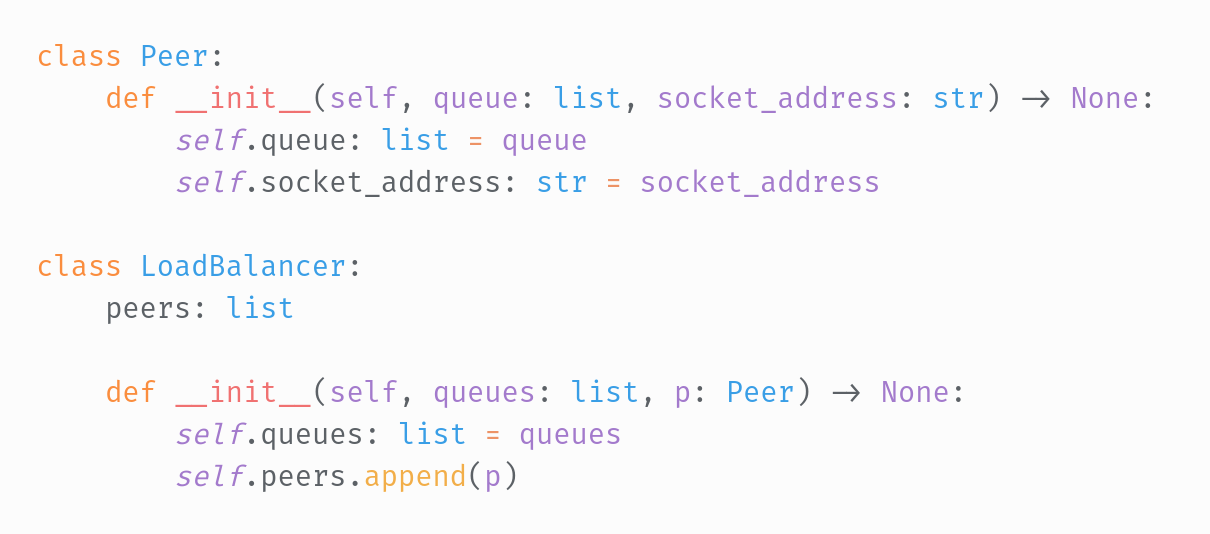
\includegraphics[width=1\textwidth]{gambar/struktur_data}
%   \caption{Penulisan struktur data pada \emph{Python}}
% \end{figure}

\begin{algorithm}[H]
  \caption{Struktur Data}\label{alg:peer-to-peer}
  \begin{algorithmic}
    \Struct{Peer} {queue: list, socket\_address: str}
      \State $self.queue \gets queue$
      \State $self.socket\_address \gets socket\_address$
    \EndStruct

    \item[] % line skip

    \Struct{LoadBalancer} {queues: list, p: Peer}
      \State $self.queues \gets queues$
      \State $self.peers.\textbf{append}(p)$
    \EndStruct
  \end{algorithmic}
\end{algorithm}



\begin{algorithm}[H]
  \caption{Algoritma Penyeimbang Antrian}\label{alg:peer-to-peer}
  \begin{algorithmic}
    \State $balancer = LoadBalancer$
    \State $queues = balancer.queues$

    \item[] % line skip

    \Function{BalancingQueue}{$list\_of\_url$}
      \For{$url \in \mathcal{} list\_of\_url[..]$}
        \State $min\_length = INFINITY$
        \State $min\_queue\_index = None$
        
        \item[] % line skip

          \For{$i, current\_queue \in enumerate(queues[..])$}
            \State $current\_length = current\_queue.length()$
              \If{$current\_length == 0$}
                \State $min\_queue\_index = i$
                \State $break$
              \ElsIf{$current\_length < min\_length$}
                \State $min\_length = current\_length$
                \State $min\_queue\_index = i$
              \EndIf
          \EndFor
      \EndFor

      \State $queues[min\_queue\_index].enqueue(url)$
    \EndFunction
  \end{algorithmic}
\end{algorithm}

\section{Skema Pendistribusian}

\begin{figure}[H]
  \centering{}
	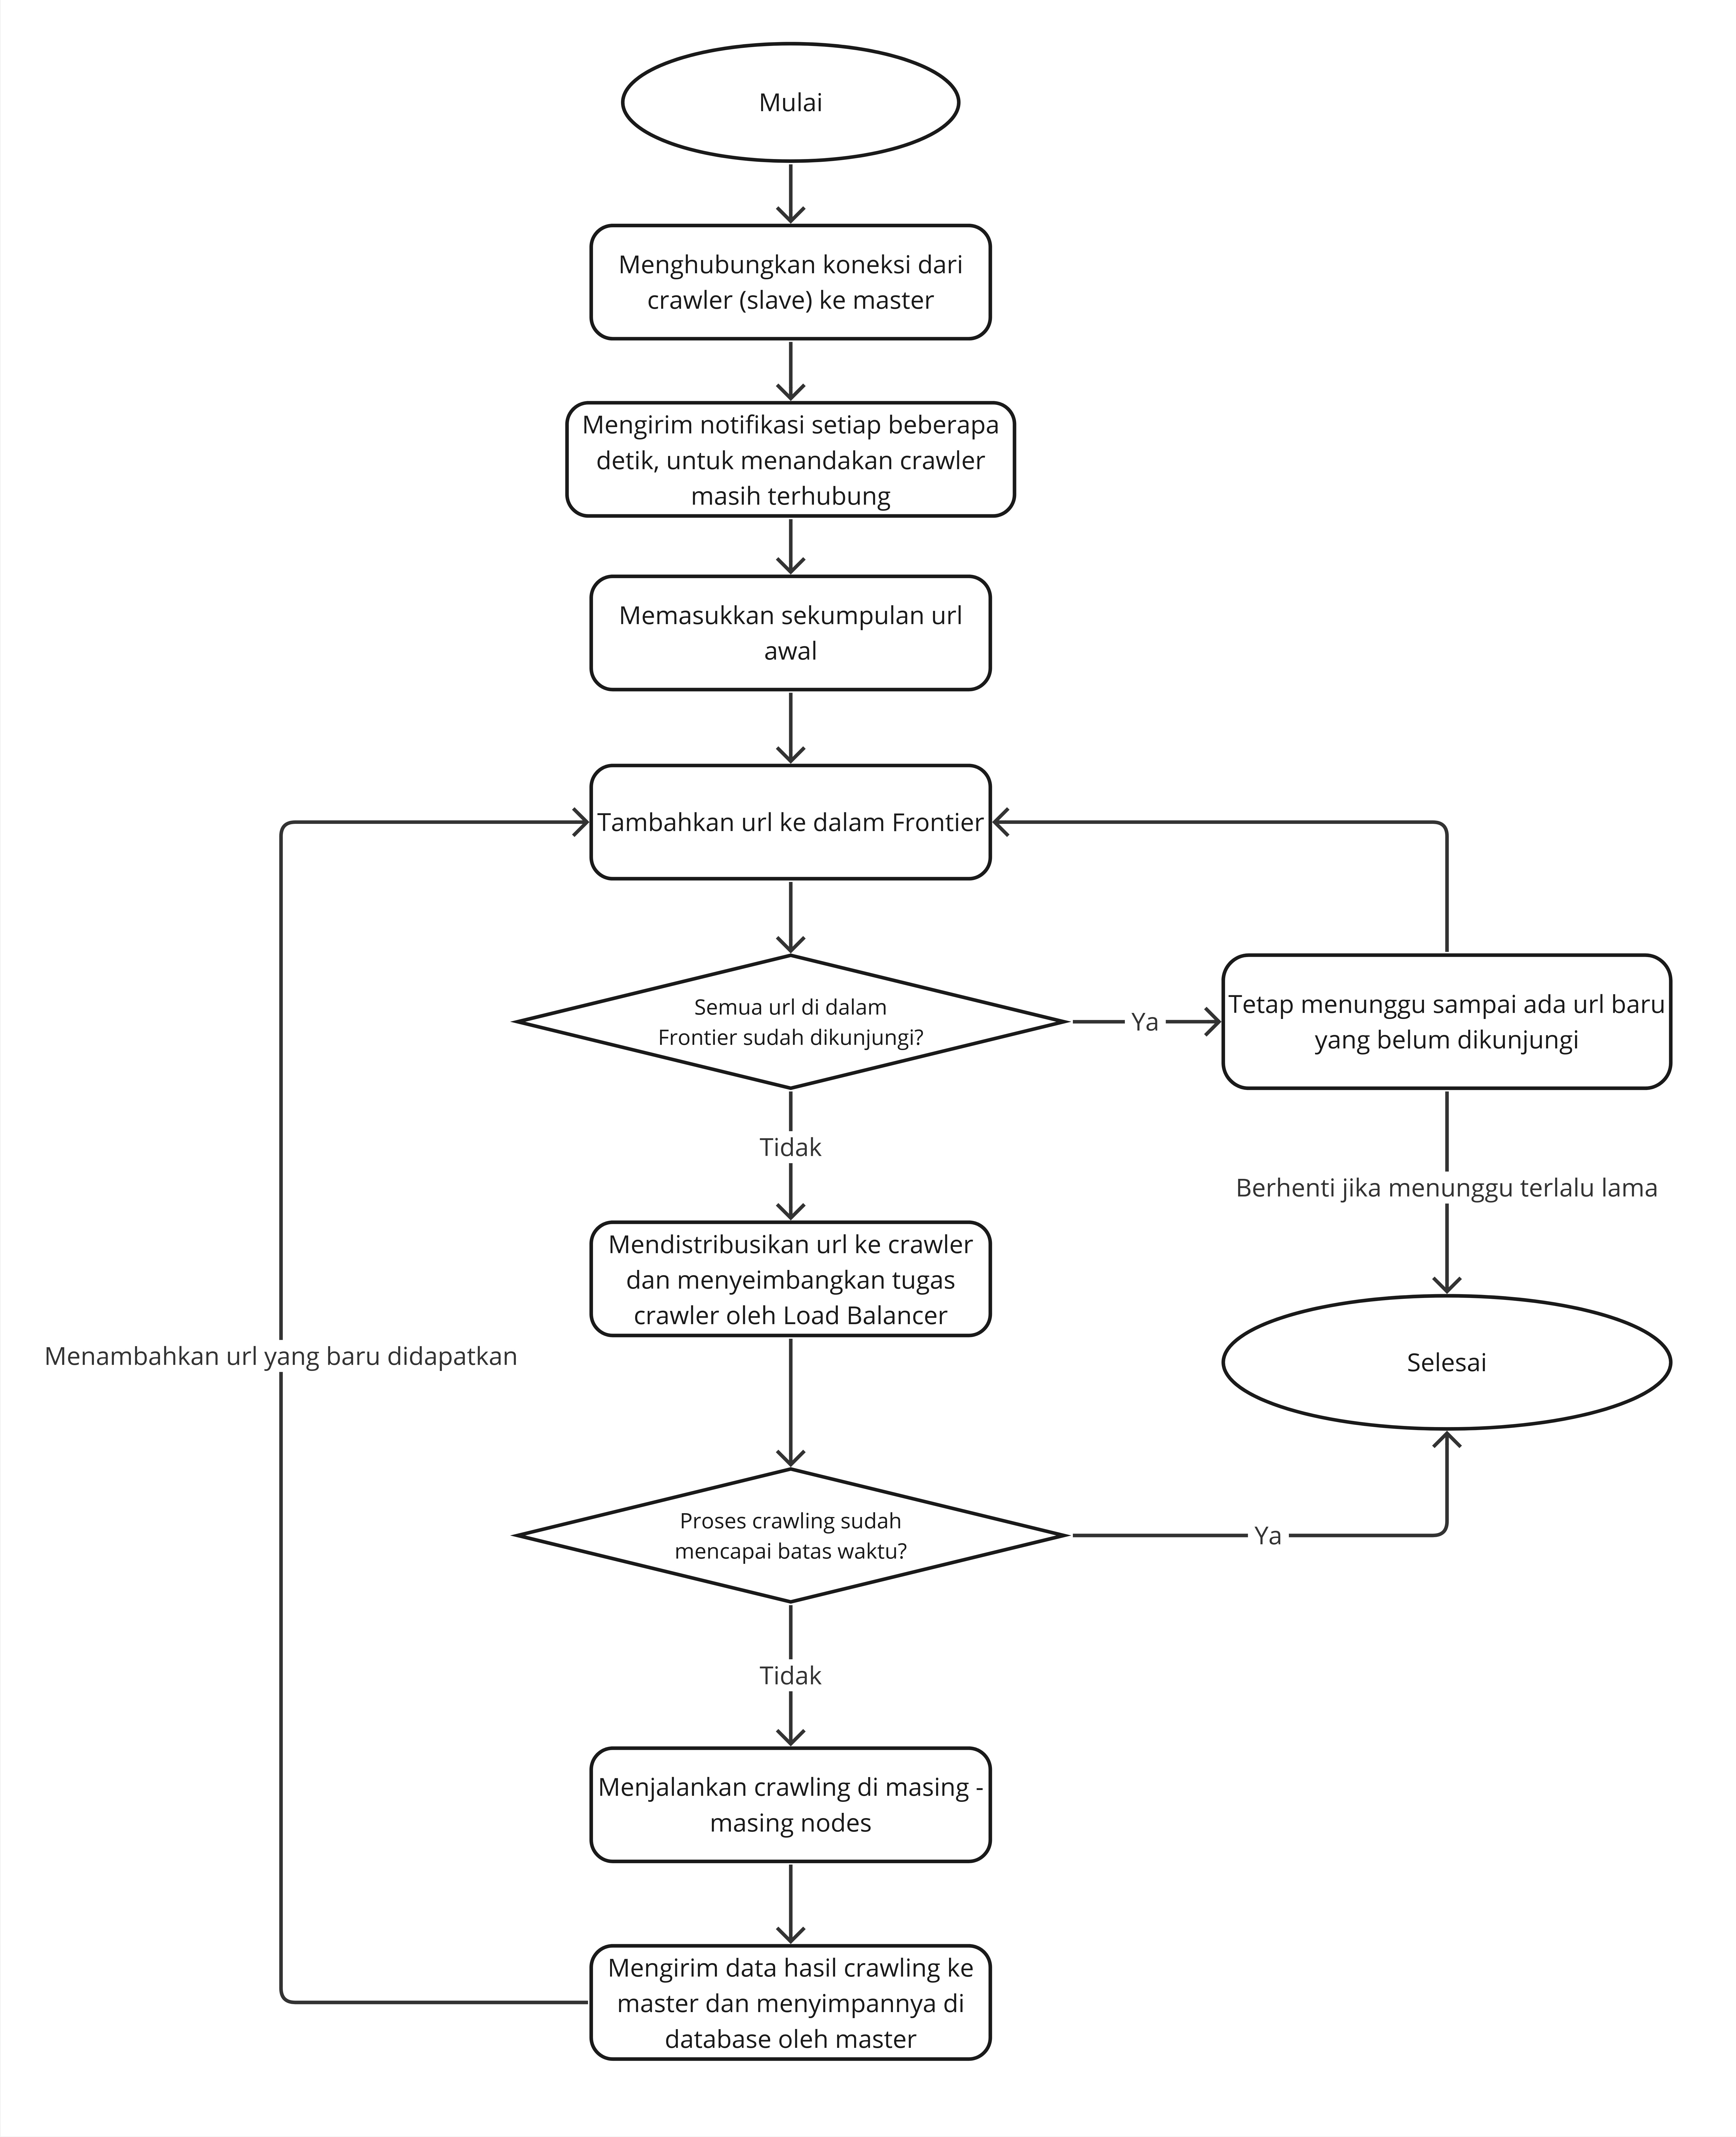
\includegraphics[width=1\textwidth]{gambar/flowchart_distributed_crawler}
  \caption{\emph{Flowchart} Skema Pendistribusian}
\end{figure}

Proses dari sistem \emph{crawler} terdistribusi dimulai dengan memasukkan sekumpulan url awal yang ingin di-\emph{crawling} ke dalam \emph{frontier}. Lalu, melakukan pengecekan terhadap url yang sudah dikunjungi di \emph{frontier}. Jika kondisinya tidak, maka akan melanjutkan untuk mendistribusikan url ke masing - masing \emph{crawler} dan menyeimbangkan beban kerjanya. Setelah itu melakukan \emph{crawling} oleh \emph{crawler} dan data disimpan di database. Data yang didapatkan dari \emph{crawling} akan dikembalikan ke \emph{frontier} yang berbentuk outgoing url dan akan dilakukan penyaringan url yang belum dikunjungi. Ketika kondisi semua url pada \emph{frontier} sudah dikunjungi maka akan menunggu sampai ada url baru yang belum dikunjungi. Akan \emph{suspend} ketika terlalu lama menunggu.

\section{Alat dan Bahan Penelitian}

Pada penelitian ini, terdapat beberapa alat yang digunakan sebagai penunjang
dalam pembuatan sistem terdistribusi dengan rincian sebagai berikut:

\begin{itemize}
  \item{Dua laptop dengan konfigurasi Intel Core i7-8650U, 16GB RAM dan Intel Core i5-8265U, 20GB RAM}
  \item{Sistem operasi \textit{Linux}}
  \item{\textit{VSCode} sebagai \textit{code editor}}
  \item{Database \textit{SQLite3} untuk menyimpan data}
  \item{\textit{Python 3}}
  \item{\textit{Virtual private server} untuk menjalankan program yang memerlukan public IP address}
\end{itemize}

\section{Tahapan Pengembangan}

\subsection{Improvisasi \emph{crawling} secara terdistribusi}

Proses improvisasi akan dilakukan dengan memodifikasi \emph{crawler} agar dapat berjalan secara terdistribusi, serta meningkatkan konsistensi data dan efisiensi sumber daya. Penelitian ini akan mengembangkan versi \emph{crawler} terdahulu (\cite{lazuardy2023search}). 

Hasil penelitian tersebut menghasilkan \emph{crawler} yang dapat menghimpun data dari bebagai halaman \emph{web} dengan tambahan \emph{multi-threading} yang dapat memaksimalkan proses kerja dengan membagi pekerjaan ke \emph{thread} yang lain. Karena hasil penelitian sebelumnya masih berjalan dalam satu perangkat saja. Dan tidak dapat berkoordinasi dengan perangkat lain. Maka, penelitian ini akan mengembangkan menjadi terdistribusi dengan mekanisme \emph{socket programming}.

\subsection{Skenario Eksperimen}

Berikut adalah skenario eksperimen agar perangkat dapat berkomunikasi satu sama lain dengan \emph{socket} dan melakukan \emph{crawling}.

\begin{enumerate}
  \item{Menjalankan program tracker pada server dengan public IP}
  \item{Menjalankan program manager pada server dengan public IP. Dan terhubung ke tracker}
  \item{Menjalankan program klien, pada server dengan public IP dan ada juga yang berjalan di private IP nantinya klien akan terkurasi yang memiliki IP public dan private. Dan terhubung ke tracker}
  \item{Manager melakukan binding koneksi, agar klien public dapat terhubung kepadanya dengan mengirim info ke tracker}
  \item{Tracker menginformasi klien public untuk mencoba terhubung ke manager dengan memberikan IP address dan portnya}
  \item{Klien public menerima informasi tersebut dan menghubungkan koneksi ke manager}
  \item{Setelah berhasil, klien public akan melakukan binding koneksi agar semua klien private dapat terhubung dengannya. Lalu memberikan informasi kepada tracker terkait hal itu}
  \item{Tracker menginformasi semua klien private untuk mencoba terhubung ke klien public dengan memberikan IP address dan portnya}
  \item{Klien private menerima informasi tersebut dan menghubungkan koneksi ke klien public}
  \item{Manager mengirim starting url yang diperlukan kepada klien public yang terhubung}
  \item{Klien public menerima starting url dan mengirimkan kepada klien private (yang aka melakukan \emph{crawling})}
  \item{Klien private melakukan \emph{crawling} dan setiap selesai satu url. Data hasilnya (konten dari web yang di-\emph{crawl} dan sekumpulan url baru yang ditemukan) akan dikirimkan ke klien public}
  \item{Klien public akan menyimpan data konten hasil \emph{crawling} di database. Dan sekumpulan url yang didapat akan dicek apakah ada duplikasi atau tidak}
  \item{Klien public kembali mengirim url yang akan di-\emph{crawling} kepada semua klien private dengan mempertimbankan "kesehatan" dari klien tersebut dan jumlah url yang berada di klien itu. Agar pembagian menjadi seimbang}
\end{enumerate}

\section{Skema Uji}

Pengujian yang akan dilakukan pada penelitian ini adalah untuk menguji konsistensi data dan efisiensi dengan crawler terdahulu.

\subsection{Sumber Data}

Sumber data yang akan digunakan dalam penelitian ini adalah situs web berita dan data yang diambil itu mencakup konten teks dari halaman web serta tautan yang berada di web tersebut.

\subsection{Metrik Pengujian}

Performa crawler terdistribusi akan dinilai menggunakan metrik berikut:
\begin{enumerate}
  \item{\textbf{Proses Komunikasi}: Proses komunikasi antara masing - masing perangkat dapat berjalan dengan sistematis.}

  \item{\textbf{Konsistensi Data}: Konsistensi data mengacu pada kemampuan mengirimkan data lengkap tanpa kehilangan atau duplikasi informasi  selama proses \emph{crawling}. Konsistensi data penting untuk memastikan keakuratan dan kelengkapan informasi yang dikumpulkan di Internet. Duplikasi atau hilangnya data dapat menyebabkan analisis yang tidak akurat dan berdampak pada keputusan berdasarkan data tersebut. Dengan pengujian analisis data tersimpan dengan membandingkan data yang dikumpulkan dengan sumber atau data yang diharapkan untuk memastikan tidak ada duplikasi.}
    
  \item{\textbf{Efisiensi dan Optimalisasi}: Efisien sumber daya dan optimalisasi jumlah data yang terkumpul dari proses \emph{crawling} terdistribusi dengan \emph{crawling} tidak terdistribusi. Ini mencakup seberapa cepat sistem dapat mengumpulkan data. Karena proses crawling yang lambat atau penggunaan sumber daya yang tidak efisien dapat menghambat kinerja \emph{crawler}. Dengan pengujian penyimpanan data, data yang dihasilkan oleh \emph{crawler} terdistribusi dapat memiliki jumlah data yang lebih banyak dalam kurun waktu yang sama, yaitu satu jam.}
\end{enumerate}

\subsection{Rancangan Eksperimen}

\begin{enumerate}
  \item{Menjalankan kedua versi crawler secara bersamaan dengan \emph{initial url web} yang sama.}
  \item{Catat jumlah data yang terkumpul dalam jangka waktu tertentu}
\end{enumerate}

% \subsection{Batasan Pengujian}

% Pengujian ini memiliki batasan pada durasi \emph{crawling} dan tidak mempertimbangkan faktor-faktor seperti kondisi jaringan yang bervariasi.

% \subsection{Implikasi Hasil}

Skema uji ini akan membantu dalam membandingkan kinerja antara crawler terdistribusi dan terdahulu (tanpa terdistribusi).
% Frontier dan \emph{load balancer} terletak pada suatu mesin yang disebut master machine. Dan untuk setiap \emph{crawler} berada pada mesin yang disebut sebagai slaves machine. Slaves machine dapat terdiri lebih dari satu. Setiap slave machine terhubung dengan master machine melalui koneksi socket.

%!TEX root = ./template-skripsi.tex
%-------------------------------------------------------------------------------
%                            	BAB IV
%               		KESIMPULAN DAN SARAN
%-------------------------------------------------------------------------------

\chapter{HASIL DAN PEMBAHASAN}

\section{Implementasi}
Berikut ini adalah keterangan \emph{flowchart} terkait tahapan penelitian yang sudah berhasil dibuat. Penyempurnaan dari \emph{flowchart} pada Gambar 3.1.

\begin{figure}[H]
  \centering{}
	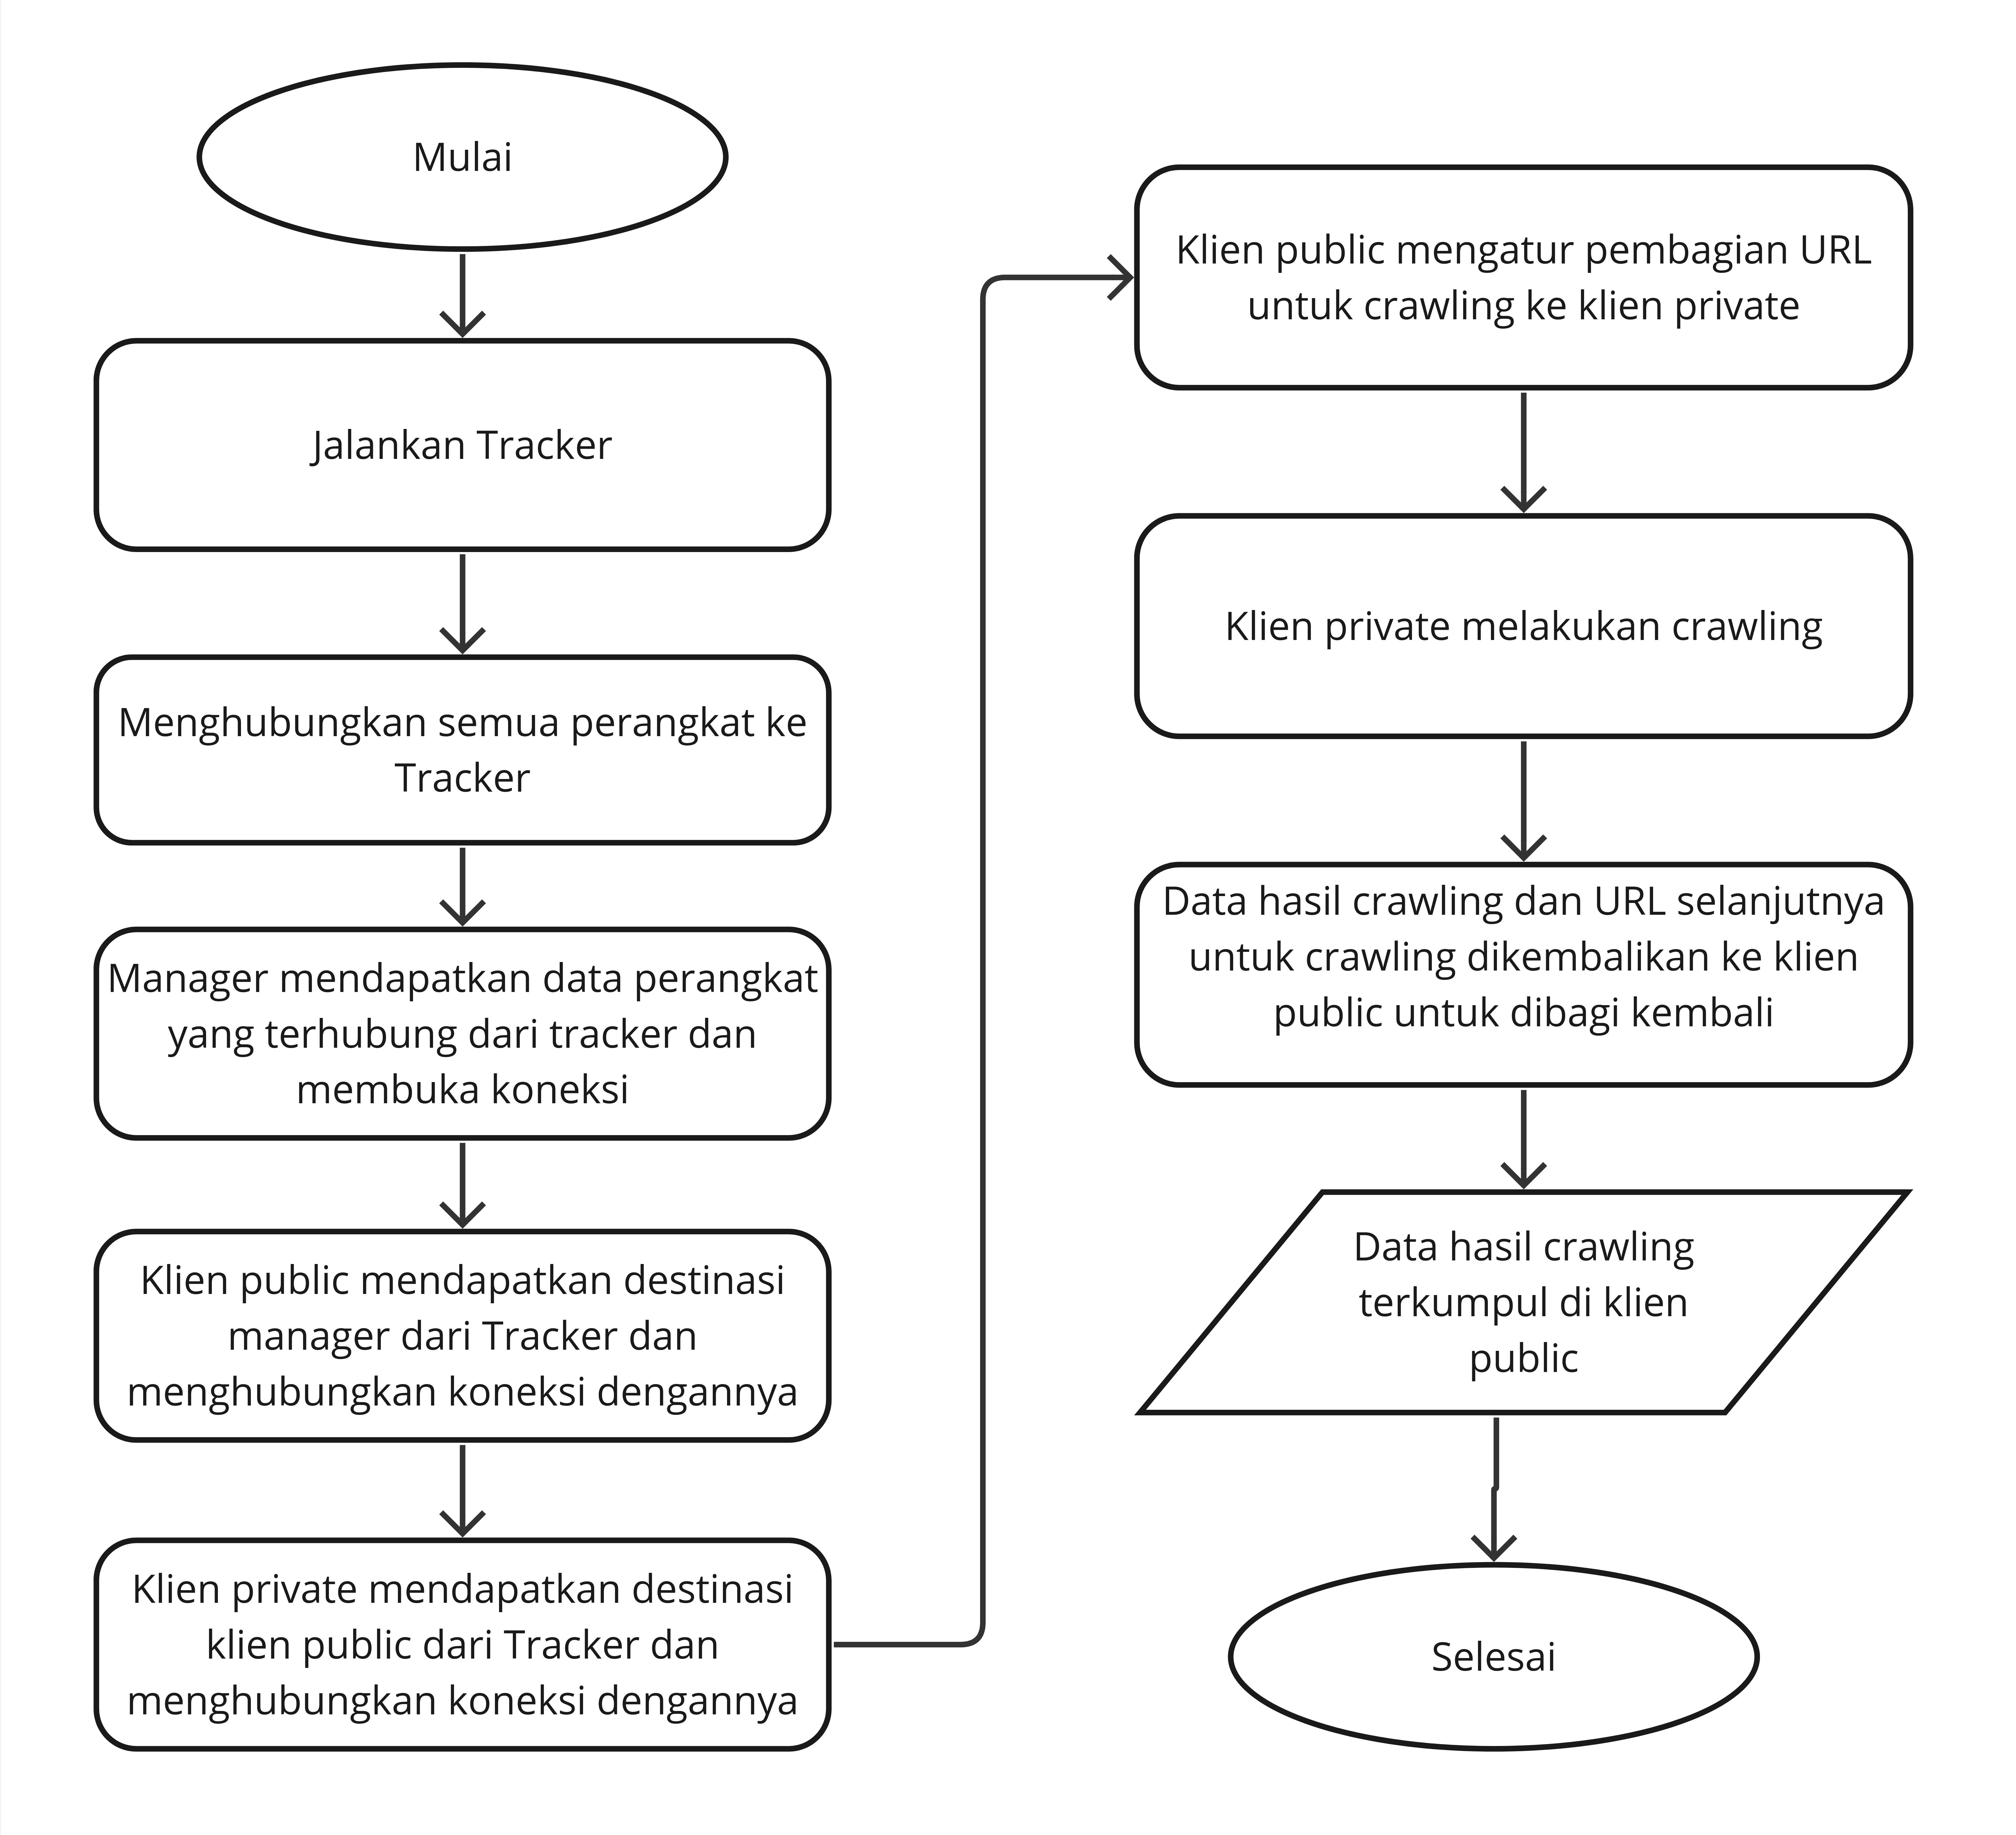
\includegraphics[width=1\textwidth]{gambar/flowchart_crawler_terdistribusi}
  \caption{\emph{Flowchart} Tahapan Penelitian yang Berhasil Dibuat}
\end{figure}

Arsitektur \emph{crawler} terdistribusi dalam penelitian ini terdiri dari lima perangkat lunak dengan konfigurasi tiga perangkat memiliki \emph{public IP address} dan dua perangkat memiliki \emph{private IP address}. Dengan pembagian perannya masing - masing, satu \emph{Tracker}, satu \emph{Manager}, dan tiga Klien. Pada penerapannya setiap program berjalan dengan bahasa pemrograman Python dan setiap proses dapat berjalan secara paralel dengan menggunakan \emph{threading}. Arsitektur ini telah mengalami modifikasi dari yang sebelumnya pada Gambar 3.2. Setelah melakukan percobaan untuk mendapatkan kondisi \emph{peer to peer}, maka dihasilkan arsitektur seperti Gambar 4.2.

\begin{figure}[H]
  \centering{}
	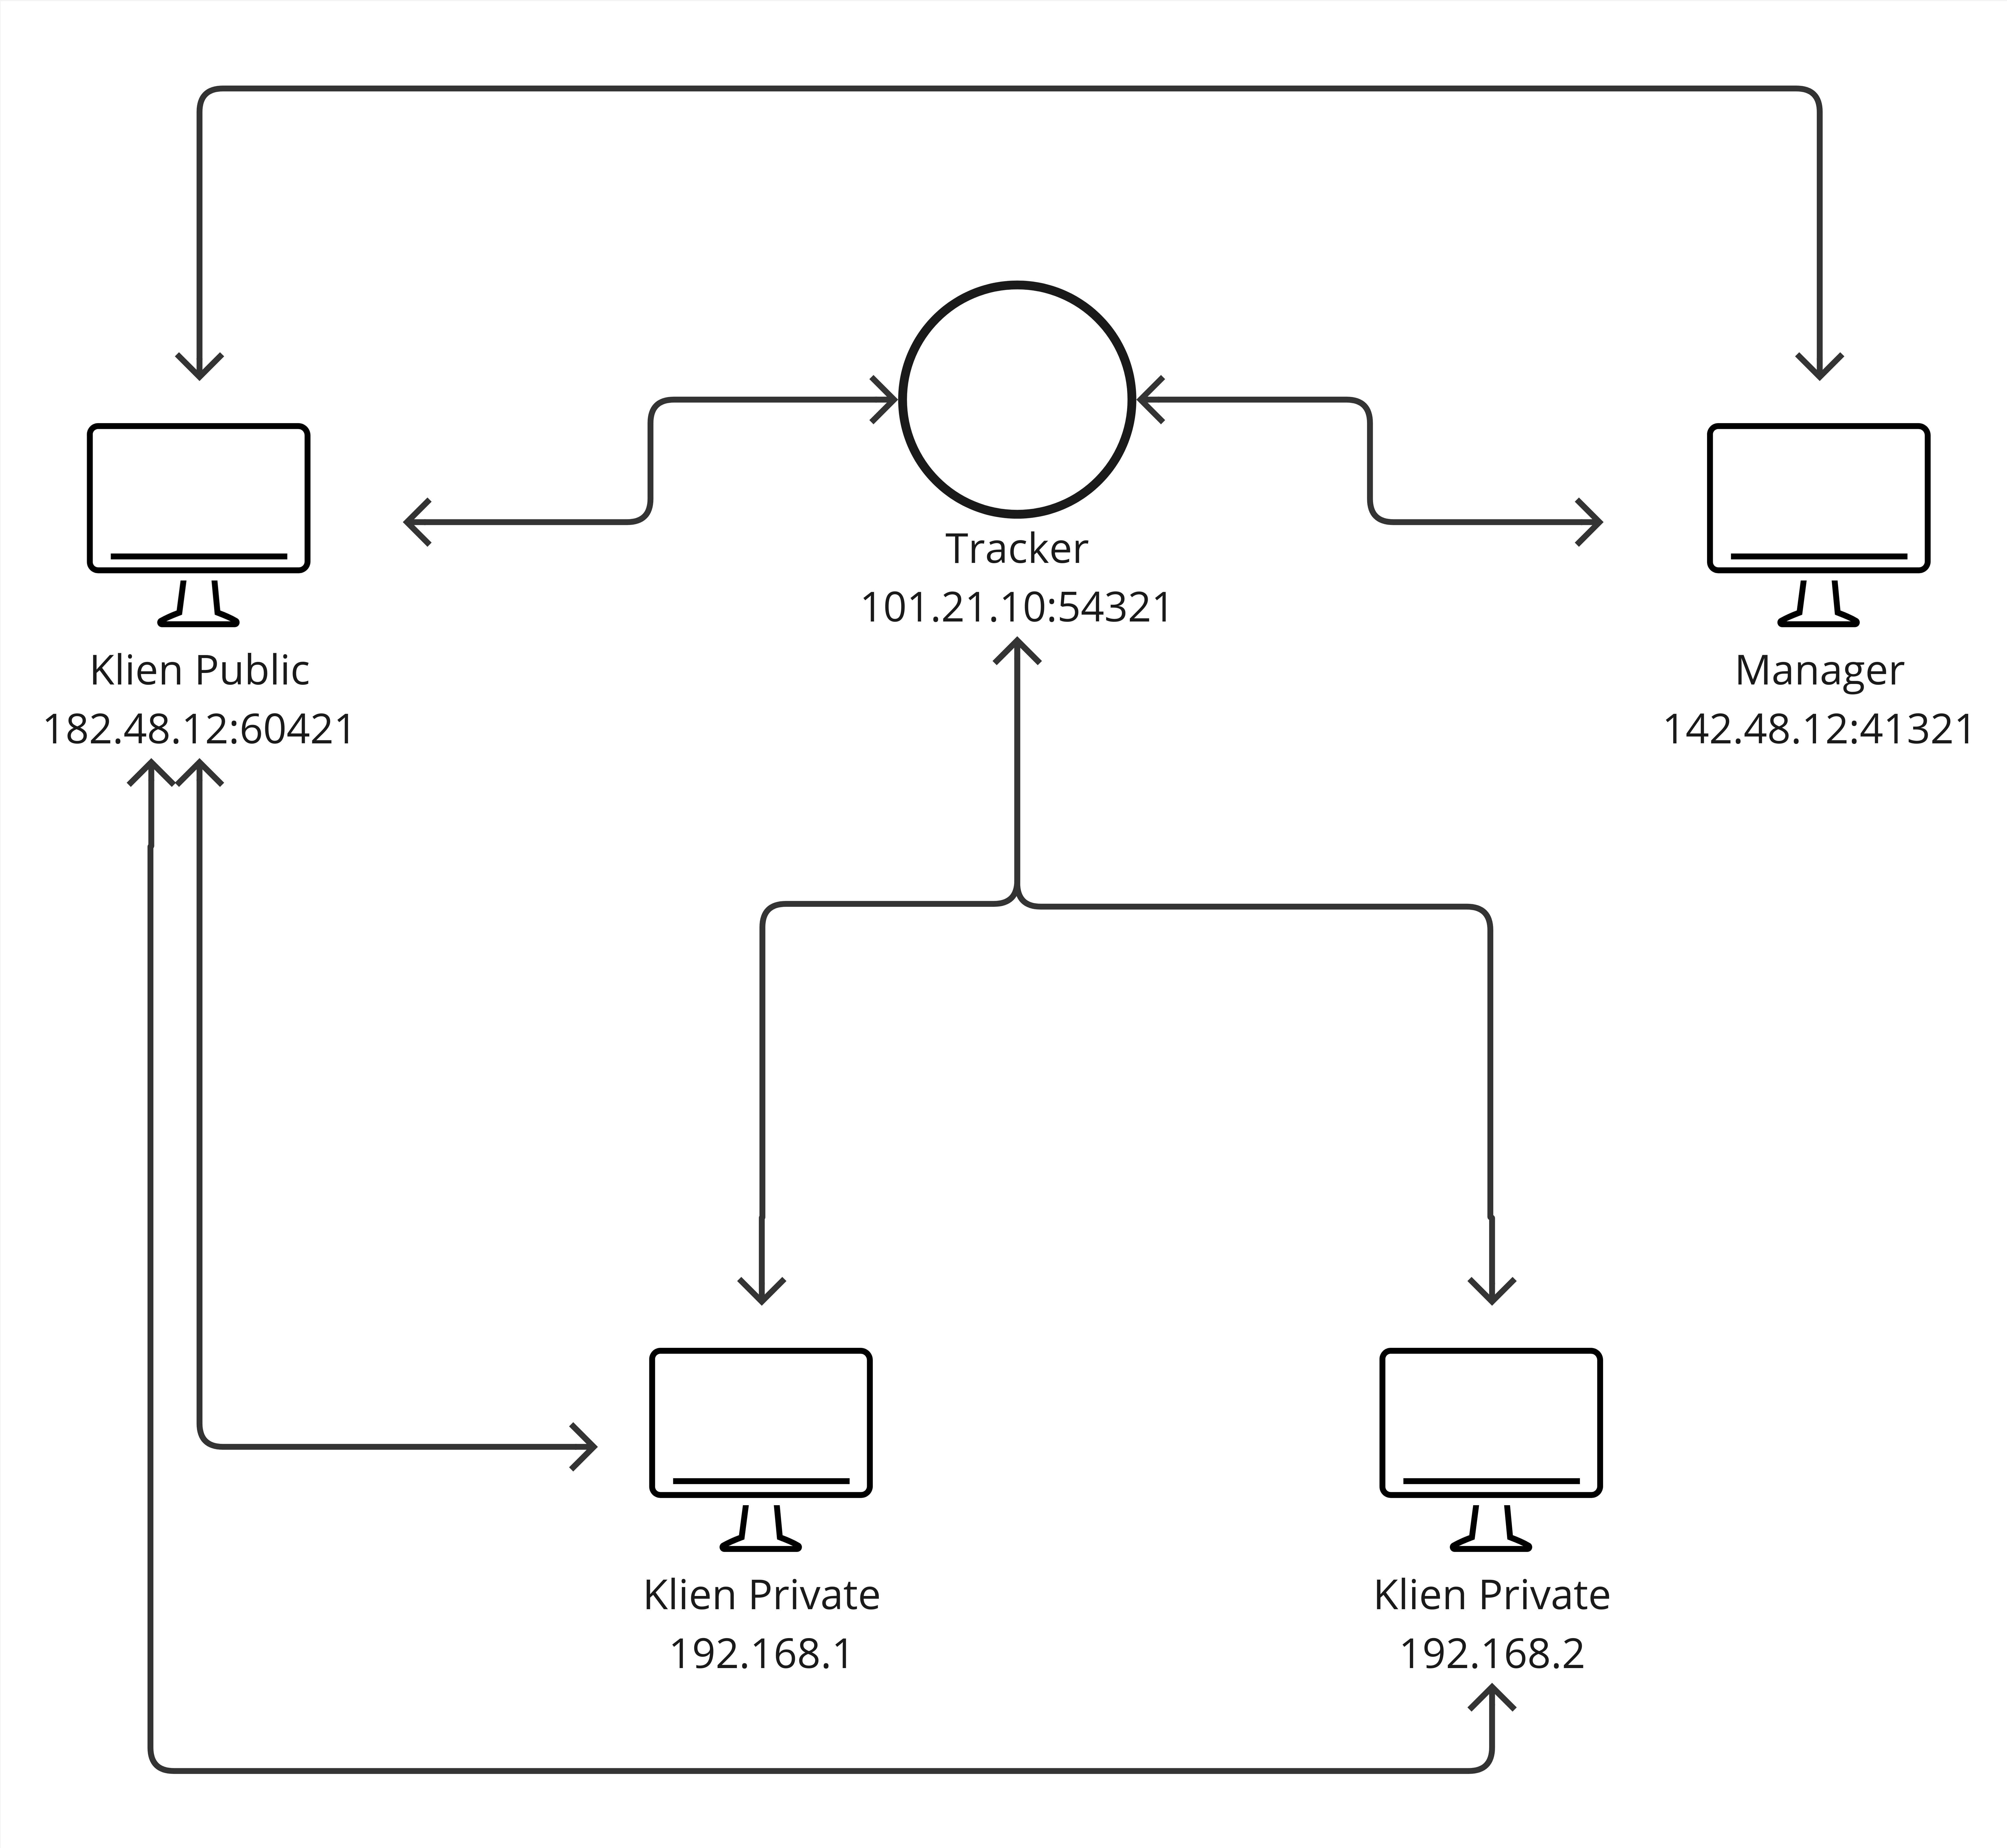
\includegraphics[width=0.6\textwidth]{gambar/arsitektur_baru}
  \caption{Arsitektur \emph{Crawler Terdistribusi}}
\end{figure}

\subsection{\emph{Tracker}}
\emph{Tracker} akan memiliki \emph{public IP address}, dikarenakan \emph{tracker} memiliki tugas sebagai jalur informasi antara perangkat yang terhubung. Setiap perangkat harus terlebih dahulu untuk terhubung melalui \emph{tracker} dan juga mengirimkan informasi apakah perangkat tersebut memiliki \emph{public IP address} atau tidak dan tipe dari perangkat tersebut, apakah dia \emph{manager} atau klien. Lalu, \emph{tracker} akan menampung semua perangkat yang terhubung. 
\clearpage

\begin{figure}[H]
	\centering{}
	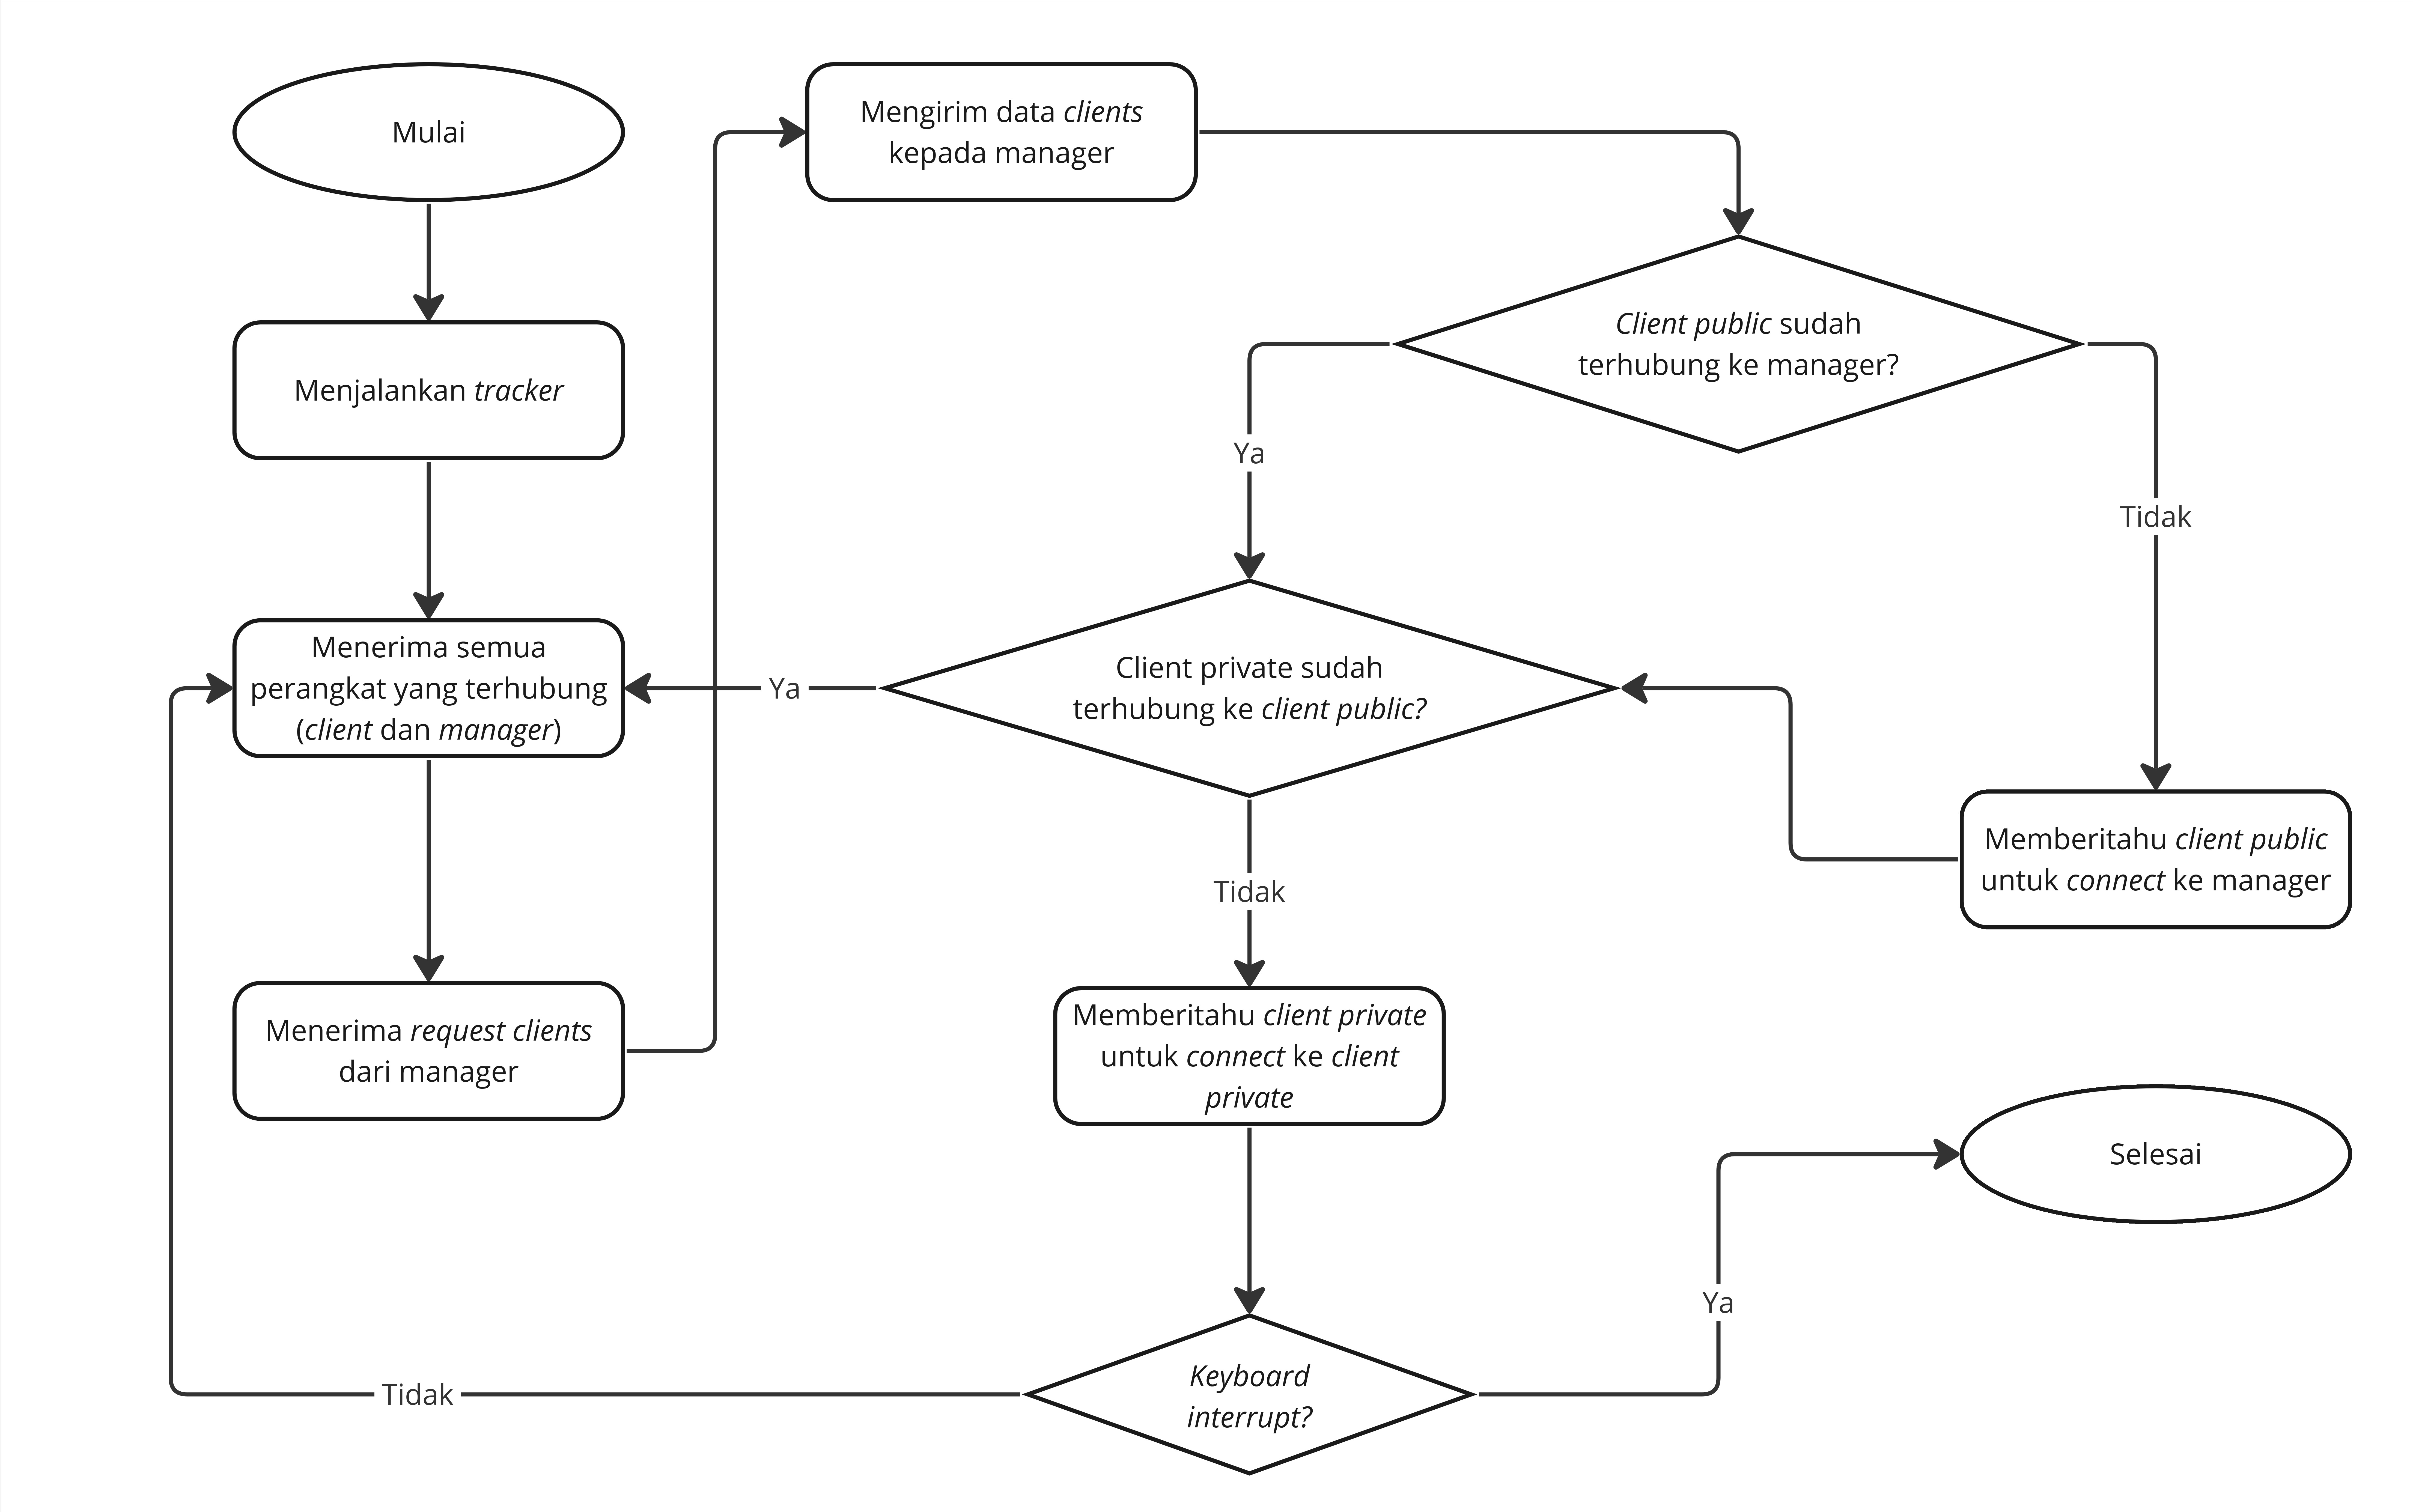
\includegraphics[width=1\textwidth]{gambar/flowchart_tracker}
	\caption{\emph{Flowchart tracker} }
\end{figure}

\begin{itemize}
	\item{Potongan kode untuk mengatur perangkat atau klien yang baru terhubung}
	\begin{figure}[H]
		\centering{}
		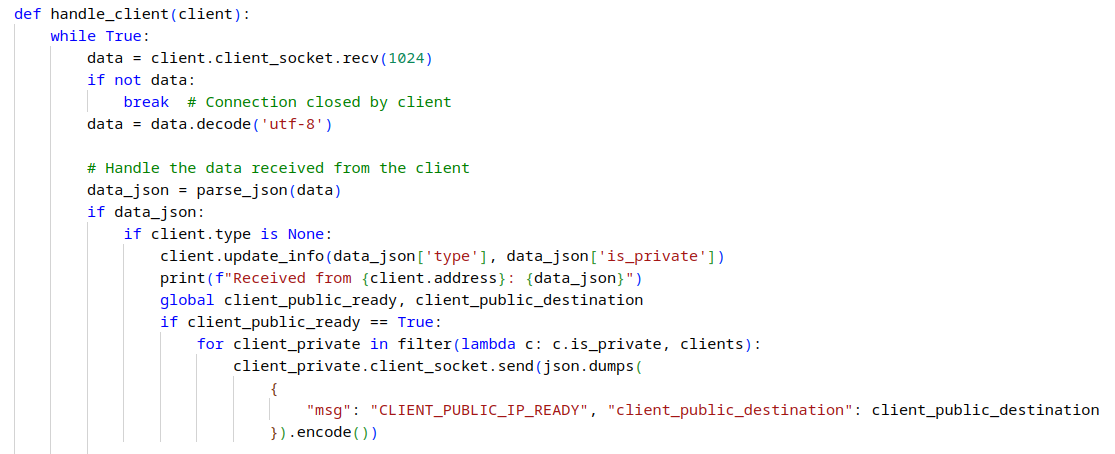
\includegraphics[width=0.8\textwidth]{gambar/kode/potongan_tracker_01}
		\caption{Potongan kode \emph{tracker} untuk klien baru terhubung}
	\end{figure}
	Setiap klien yang terhubung akan diterima oleh \emph{tracker} dan pesannya akan disimpan.

	\clearpage
	\item{Potongan kode untuk merespons \emph{manager} yang meminta kumpulan klien}
	\begin{figure}[H]
		\centering{}
		\includegraphics[width=0.8\textwidth]{gambar/kode/potongan_tracker_02}
		\caption{Potongan kode \emph{tracker} merespons \emph{manager} yang meminta kumpulan klien } 
	\end{figure}
	Setiap kali manager meminta data klien kepada \emph{tracker}. \emph{Tracker} akan merespons pesan tersebut dengan mengirim data klien kepada manager.

	\item{Potongan kode untuk merespons \emph{manager} sudah siap membuka koneksi}
	\begin{figure}[H]
		\centering{}
		\includegraphics[width=0.8\textwidth]{gambar/kode/potongan_tracker_03}
		\caption{Potongan kode \emph{tracker} merespons \emph{manager} sudah siap membuka koneksi}
	\end{figure}
	Manager memberitahukan \emph{tracker} bahwa manager sudah siap membuka koneksi untuk dihubungkan oleh klien \emph{public}. 

	\item{Potongan kode untuk memberitahu klien \emph{private} bahwa dapat terhubung ke \emph{manager} }
	\begin{figure}[H]
		\centering{}
		\includegraphics[width=1\textwidth]{gambar/kode/potongan_tracker_04}
		\caption{Potongan kode \emph{tracker} memberitahu klien \emph{private} untuk \emph{connect}}
	\end{figure}
	Setelah manager sudah siap untuk dihubungkan dengan klien \emph{public}. Lalu klien \emph{public} mengirimkan kembali info ke \emph{tracker} bahwa sudah terhubung ke manager, Lalu manager mengirim info ke klien \emph{private} untuk dapat terhubung ke klien \emph{public}.

\end{itemize} 

\subsection{\emph{Manager}}
\emph{Manager} akan memiliki \emph{public IP address}, dikarenakan \emph{manager} memiliki tugas untuk mengatur perangkat terhubung yang nantinya akan memiliki \emph{public IP address}. \emph{Manager} juga perlu untuk terhubung ke \emph{tracker}. \emph{Manager} mendapatkan klien yang terhubung dengan meminta data klien yang terhubung kepada \emph{tracker}. Lalu, \emph{tracker} akan mengirimkan data klien yang terhubung. \emph{Manager} akan membuka koneksi untuk klien yang nantinya memiliki \emph{public IP address} untuk terhubung dengannya.

\begin{figure}[H]
	\centering{}
	\includegraphics[width=0.8\textwidth]{gambar/flowchart_manager}
	\caption{\emph{Flowchart manager} }
\end{figure}

\begin{itemize}
	\item{Potongan kode untuk menerima kumpulan klien dari \emph{tracker} dan mengirim kembali ke \emph{tracker} bahwa \emph{manager} sudah bersedia untuk dihubungkan dengan klien \emph{public}}
	\begin{figure}[H]
		\centering{}
		\includegraphics[width=0.8\textwidth]{gambar/kode/potongan_manager_01}
		\caption{Potongan kode \emph{manager} yang menerima data klien dan menginformasikan \emph{tracker}}
	\end{figure}

	\item{Potongan kode untuk membuka koneksi agar klien \emph{public} dapat terhubung dan inisisasi \emph{starting url}}
	\begin{figure}[H]
		\centering{}
		\includegraphics[width=0.8\textwidth]{gambar/kode/potongan_manager_02}
		\caption{Potongan kode \emph{manager} untuk membuka koneksi agar klien \emph{public} dapat terhubung}
	\end{figure}
\end{itemize}

\subsection{Klien}
Klien dapat memiliki \emph{public} dan \emph{private IP address}. Dalam penelitian ini terdapat 1 klien dengan \emph{public IP address} dan 2 klien dengan \emph{private IP address}, yang nantinya klien dengan \emph{private IP address} akan menjadi \emph{worker} yang melakukan \emph{crawling}. Setelah klien \emph{public} terhubung dengan \emph{tracker}. Dan \emph{tracker} juga sudah mendeteksi adanya \emph{manager} yang sudah terhubung. Maka, \emph{tracker} akan mengirim informasi \emph{manager} kepada klien tersebut. Agar klien tersebut dapat terhubung dengan \emph{manager}. Untuk klien \emph{private} nantinya akan terhubung dengan klien \emph{public} setelah mendapatkan informasi dari \emph{tracker} bahwa klien \emph{public} sudah siap untuk dihubungkan. Klien \emph{private} akan melakukan \emph{crawling} yang mana pembagian url-nya akan diatur oleh klien \emph{public}. Data hasil \emph{crawling} akan dikembalikan ke klien \emph{public} untuk disatukan. 

Proses \emph{crawling} harus dilakukan oleh klien \emph{private} dikarenakan jika dilakukan oleh klien \emph{public} akan berdampak pada \emph{Domain Name System} (DNS) klien tersebut yang dapat diblokir. Karena situs web memiliki syarat dan kebijakan yang memiliki batasan terhadap \emph{crawling} otomatis, dan dengan penggunaan klien \emph{private} dapat meminimalkan risiko. Klien \emph{private} juga membantu untuk menghindari batasan tingkat permintaan (\emph{rate limiting}), karena kalau dengan klien \emph{public} peraturannya akan lebih ketat karena terikat dari penyedia layanan internet atau server layanan.

\begin{figure}[H]
	\centering{}
	\includegraphics[width=1\textwidth]{gambar/flowchart_client}
	\caption{\emph{Flowchart client} }
\end{figure}
\clearpage

\begin{itemize}
	\item{Struktur direktori dari kode klien}
	\begin{figure}[H]
		\centering{}
		\includegraphics[width=0.4\textwidth]{gambar/kode/potongan_client_01}
		\caption{Struktur direktori kode klien}
	\end{figure}
\end{itemize}

Pada direktori \emph{"client"} terdapat tiga buah folder penunjang. \emph{"crawling"}, folder ini berisikan fungsi utama untuk melakukan \emph{crawling} serta utilitasnya. \emph{"database"}, folder ini berisikan fungsi untuk mengelola basis data, mulai dari menentukan table serta attributnya. Di folder tersebut juga terdapat \emph{"public\_client"} folder, yang berguna untuk klien \emph{public} mendefinisikan basis datanya. \emph{"methods"}, pada folder ini berisikan metode yang digunakan untuk melakukan \emph{scraping data} dari internet berdasar url yang ditentukan. 

File utama yang akan dijalankan adalah file \emph{"client.py"}. Pada file tersebut berisikan proses dari klien penentuan \emph{public} atau \emph{private} klien berdasarkan perangkat yang menjalankan program, terhubung dengan \emph{tracker}, dan melakukan komunikasi antar klien. Juga terdapat file \emph{".env"} sebagai penentuan ekosistem program, seperti berapa lamanya \emph{worker} atau klien \emph{private} akan bekerja. File \emph{"requirements.txt"} berisikan modul - modul yang diperlukan untuk menjalankan program. File \emph{"slave.py"} juga tidak kalah penting, karena didalamnya terdapat fungsi - fungsi untuk membantu pengiriman data ke klien \emph{public}. Pada penelitian ini akan lebih mendalam membahas tentang proses distribusinya. Karena untuk metode \emph{crawling} sebagian besar akan sama dengan penelitian terdahulu (\cite{lazuardy2023search}).
\clearpage

\begin{itemize}
	\item{Fungsi untuk mendapatkan IP \emph{address} apakah \emph{public} atau \emph{private}}
	\begin{figure}[H]
		\centering{}
		\includegraphics[width=1\textwidth]{gambar/kode/potongan_client_00}
		\caption{Fungsi untuk mendapatkan IP \emph{address} apakah \emph{public} atau \emph{private}}
	\end{figure}
\end{itemize}
Pada fungsi ini dapat menentukan IP \emph{address}-nya dengan cara mendapatkan \emph{socket address} yang sudah terhubung dengan \emph{socket} lain. Dan \emph{address}-nya akan dibandingkan dengan IP address \emph{private}. Kalau tidak sama, berarti \emph{address} tersebut adalah \emph{public}. Kalau sama, berarti \emph{private}. 

\clearpage
\subsubsection{Klien \emph{Public}}

\begin{itemize}
	\item{Pendeklarasian kelas \emph{Client}}
	\begin{figure}[H]
		\centering{}
		\includegraphics[width=1\textwidth]{gambar/kode/potongan_client_02}
		\caption{Pendeklarasian kelas \emph{Client}}
	\end{figure}

	\item{Pendeklarasian kelas \emph{LoadBalancer}}
	\begin{figure}[H]
		\centering{}
		\includegraphics[width=0.8\textwidth]{gambar/kode/potongan_client_03}
		\caption{Pendeklarasian kelas \emph{LoadBalancer}}
	\end{figure}

	\clearpage
	\item{Potongan kode \emph{public} untuk merespons komunikasi dengan \emph{tracker} untuk mendapatkan informasi ketika \emph{manager ready} dan menginformasikan klien \emph{private} untuk terhubung}
	\begin{figure}[H]
		\centering{}
		\includegraphics[width=1\textwidth]{gambar/kode/potongan_client_09}
		\caption{Potongan kode klien \emph{private}}
	\end{figure}

	\item{Potongan kode klien \emph{public} mencoba terhubung dengan \emph{manager}}
	\begin{figure}[H]
		\centering{}
		\includegraphics[width=1\textwidth]{gambar/kode/potongan_client_10}
		\caption{Potongan kode klien \emph{public} mencoba terhubung dengan \emph{manager}}
	\end{figure}
	\clearpage

	\item{Potongan kode komunikasi antar klien serta mengirimkan url pertama untuk di-\emph{crawling} kepada klien \emph{private}}
	\begin{figure}[H]
		\centering{}
		\includegraphics[width=1\textwidth]{gambar/kode/potongan_client_04}
		\caption{Potongan kode komunikasi antar klien}
	\end{figure}
	Klien \emph{public} akan mengatur klien \emph{private} yang terhubung. Menyimpan \emph{unique identifier}-nya, akan dipastikan bahwa tidak ada klien \emph{private} dengan address yang sama terhubung. Dan tentunya akan menghapus klien \emph{private} yang sudah tidak lagi terhubung lagi dengan klien \emph{public}. Pencatatan jumlah url untuk setiap klien \emph{private} juga dipertimbangkan.
	
	Serta pengiriman data akan di-\emph{encode} ke JSON dan di-\emph{compress} agar data yang dikirimkan tidak begitu besar. Setiap data yang diterima oleh klien \emph{public} pun juga akan di-\emph{decompress}. 

	\item{Potongan kode klien \emph{public} menerima data hasil \emph{crawling} yang diberikan oleh klien \emph{private} serta memasukkan informasi terkait ke dalam database}
	\begin{figure}[H]
		\centering{}
		\includegraphics[width=0.8\textwidth]{gambar/kode/potongan_client_05}
		\caption{Potongan kode klien \emph{public} menerima data hasil \emph{crawling}}
	\end{figure}

	\item{Fungsi untuk pengecekan duplikasi url yang didapatkan dari hasil \emph{crawling}}
	\begin{figure}[H]
		\centering{}
		\includegraphics[width=1\textwidth]{gambar/kode/potongan_client_06}
		\caption{Fungsi untuk pengecekan duplikasi url yang didapatkan dari hasil \emph{crawling}}
	\end{figure}

	\item{Potongan kode klien \emph{public} mengirimkan url yang akan di-\emph{crawling} ke klien \emph{private} dengan mempertimbangkan kondisi dari klien tersebut berdasarkan kecepatan \emph{crawling}. Klien yang lambat akan dikirim sedikit url untuk mengurangi bebannya. Sedangkan, klien yang cepat akan mendapatkan jumlah tugas lebih banyak.}

	\begin{figure}[H]
		\centering{}
		\includegraphics[width=1\textwidth]{gambar/kode/potongan_client_07}
		\caption{Potongan kode klien \emph{public} mengirimkan url yang akan di-\emph{crawling}}
	\end{figure}
	Setiap beberapa detik sekali klien \emph{public} akan mengirimkan url yang akan di-\emph{crawling} oleh klien \emph{private}. Url yang dikirim sudah dipastikan tidak terduplikasi dan dilakukan \emph{compress}. Penentuan pengiriman jumlah url juga ditentukan dari "kesehatan" dari klien \emph{private}. Kalau kondisinya "sehat", maka akan mendapatkan 30 url setiap kiriman dan sebaliknya akan mendapatkan 20 url.

	\clearpage
	\item{Fungsi untuk pengecekan "kesehatan" dari setiap klien yang terhubung}
	\begin{figure}[H]
		\centering{}
		\includegraphics[width=1\textwidth]{gambar/kode/potongan_client_08}
		\caption{Fungsi untuk pengecekan "kesehatan" dari setiap klien yang terhubung}
	\end{figure}
\end{itemize}

\subsubsection{Klien \emph{Private}}

\begin{itemize}
	\item{Fungsi untuk klien \emph{private} terhubung ke klien \emph{public}}
	\begin{figure}[H]
		\centering{}
		\includegraphics[width=1\textwidth]{gambar/kode/potongan_client_11}
		\caption{Fungsi untuk klien \emph{private} terhubung ke klien \emph{public}}
	\end{figure}
	Ketika pertama kali klien \emph{private} terhubung ke klien \emph{public}. Maka akan mengirimkan \emph{unique identifier} untuk membedakan client yang terhubung. Dan tidak lupa pula untuk di-\emph{compress}.

	\clearpage
	\item{Fungsi untuk klien \emph{private} menerima url yang akan di-\emph{crawling} dari klien \emph{public}}
	\begin{figure}[H]
		\centering{}
		\includegraphics[width=1\textwidth]{gambar/kode/potongan_client_12}
		\caption{Fungsi untuk klien \emph{private} menerima url yang akan di-\emph{crawling} dari klien \emph{public}}
	\end{figure}

	\clearpage
	\item{Potongan kode dari fungsi untuk klien \emph{private} mengirim url hasil \emph{crawling} ke klien \emph{public}}
	\begin{figure}[H]
		\centering{}
		\includegraphics[width=0.8\textwidth]{gambar/kode/potongan_client_13}
		\caption{Potongan kode dari fungsi untuk klien \emph{private} mengirim url hasil \emph{crawling} ke klien \emph{public}}
	\end{figure}

	\clearpage
	\item{Potongan kode dari fungsi untuk klien \emph{private} melakukan \emph{scraping} halaman web}
	\begin{figure}[H]
		\centering{}
		\includegraphics[width=1\textwidth]{gambar/kode/potongan_client_14}
		\caption{Potongan kode untuk klien \emph{private} melakukan \emph{scraping} halaman web}
	\end{figure}
\end{itemize}

\section{Pengujian}

Pada penelitian ini akan terfokus untuk menguji proses komunikasi yang terjadi, konsistensi data, efisiensi sumber daya dan optimalisasi data . Dijalankan proses \emph{crawling} selama satu jam. Pada \emph{crawler} individual dan \emph{crawler} terdistribusi. Pengujian dilakukan dengan \emph{initial url}: "https://www.detik.com/". 


\begin{table}[H]
	\begin{center}
		\caption{\label{tabel:hasil_crawling} Hasil \textit{crawling} selama satu jam}
		\begin{tabular}{|c|c|c|} 
			\hline
				Jenis \textit{Crawler} & \textit{Total Rows} & \textit{Unique Rows} \\ 
			\hline
				\textit{Crawler} Individual & 7069 & 7069 \\
			\hline
				2 \textit{Crawler} Terdistribusi & 9175 & 9175 \\
			\hline
		\end{tabular}
	\end{center}
\end{table}

% \begin{figure}[H]
% 	\centering{}
% 	\includegraphics[width=0.4\textwidth]{gambar/hasil/hasil_satu_jam_crawler_individual}
% 	\caption{Hasil dari \emph{crawling} dengan \emph{crawler} individual selama satu jam}
% \end{figure}

% \begin{figure}[H]
% 	\centering{}
% 	\includegraphics[width=0.4\textwidth]{gambar/hasil/hasil_satu_jam_crawler_terdistribusi_dua_crawler}
% 	\caption{Hasil dari \emph{crawling} dengan \emph{crawler} terdistribusi selama satu jam dengan skema dua \emph{crawler}}
% \end{figure}

\subsection{Proses Komunikasi}
Berikut adalah proses komunikasi pada setiap perangkat:
\begin{itemize}
	\item{Proses komunikasi pada \emph{tracker}}
	\begin{figure}[H]
		\centering{}
		\includegraphics[width=0.8\textwidth]{gambar/kode/uji_tracker}
		\caption{Proses komunikasi pada \emph{tracker}}
	\end{figure}

	\item{Proses komunikasi pada \emph{manager}}
	\begin{figure}[H]
		\centering{}
		\includegraphics[width=0.8\textwidth]{gambar/kode/uji_manager}
		\caption{Proses komunikasi pada \emph{manager}}
	\end{figure}

	\item{Proses komunikasi pada klien \emph{public}}
	\begin{figure}[H]
		\centering{}
		\includegraphics[width=0.8\textwidth]{gambar/kode/uji_client_public}
		\caption{Proses komunikasi pada klien \emph{public}}
	\end{figure}

	\item{Proses komunikasi pada klien \emph{private}}
	\begin{figure}[H]
		\centering{}
		\includegraphics[width=0.6\textwidth]{gambar/kode/uji_client_private}
		\caption{Proses komunikasi pada klien \emph{private}}
	\end{figure}
\end{itemize}

\subsection{Konsistensi Data}
Berdasarkan Tabel 4.1, didapatkan hasil data url yang di-\emph{crawling} itu unik dan tidak ada duplikasi. Berdasarkan hasil perhitungan sebagai berikut.
\[
\text{Jumlah baris yang terduplikasi} = \emph{Total Rows} - \emph{Unique Rows} = 9175 - 9175 = 0
\]

\subsection{Efisien Sumber Daya dan Optimalisasi Data}
Berdasarkan Tabel 4.1, didapatkan hasil peningkatan jumlah data dengan waktu yang relatif sama, yaitu satu jam. Pada \emph{crawler} individual didapatkan jumlah baris data dalam tabel database sebanyak 7069 dan pada \emph{crawler} terdistribusi didapatkan jumlah baris data dalam tabel database sebanyak 9175. Terdapat peningkatan jumlah data yang didapatkan oleh \emph{crawler} terdistribusi. Penambahan total data yang terkumpul dapat dicapai beriringan dengan sumber daya yang digunakan secara efisien.

$\text{Persentase peningkatan data} = \left( \frac{9175 - 7069}{7069} \right) \times 100 \approx 30.0\%$

\section{Analisis Hasil}
Berdasarkan proses perbandingan \emph{crawling} yang berjalan selama satu jam, analisis hasil pengujian adalah sebagai berikut:

\begin{enumerate}
	\item Proses komunikasi antar perangkat berjalan dengan sistematis.

	\item Data yang dihasilkan dari \emph{crawler} terdistribusi lebih banyak daripada \emph{crawler} individual. Didapatkan sekitar 30\% lebih banyak.
	
	\item Duplikasi data dapat terhindarkan saat mengelola lebih dari satu \emph{crawler} dengan melakukan \emph{crawling} berdasarkan url yang diterima dari pengelola (klien \emph{public}) dan mengembalikan temuan url baru kepada pengelola.

	\item Efisiensi sumber daya dan optimalisasi data dapat tercapai, hanya dengan melakukan \emph{crawling} selama satu jam. Bisa lebih dari satu \emph{crawler} yang berjalan di satu waktu yang bersamaan. Peningkatan tersebut juga dipengaruhi oleh latensi jaringan, \emph{overhead} koordinasi, dan potensi \emph{bottleneck}.

	\item Proses penyatuan data menjadi \emph{centralized} pada satu perangkat, yang mana merupakan penggabungan dari setiap \emph{crawler} yang melakukan pekerjaan.
\end{enumerate}

Hasil perbandingan \emph{crawler} individual dengan \emph{crawler} terdistribusi menunjukkan hasil yang baik. Peningkatan efisiensi dapat diraih dengan menerapkan metode terdistribusi. Ada hal yang harus dibayar dalam meningkatkan efisiensi, walaupun perbedaan yang terlihat hanya 30\% tapi itu merupakan hal yang baik karena hasil akhirnya mengalami peningkatan. 

% Baris ini digunakan untuk membantu dalam melakukan sitasi
% Karena diapit dengan comment, maka baris ini akan diabaikan
% oleh compiler LaTeX.
\begin{comment}
\bibliography{daftar-pustaka}
\end{comment}

%!TEX root = ./template-skripsi.tex
%-------------------------------------------------------------------------------
%                            	BAB IV
%               		KESIMPULAN DAN SARAN
%-------------------------------------------------------------------------------

\chapter{KESIMPULAN DAN SARAN}

\section{Kesimpulan}
Berdasarkan hasil implementasi dan pengujian terhadap \emph{crawler} terdistribusi. Maka diperoleh kesimpulan seperti berikut:

\begin{enumerate}
	\item Pembuatan \emph{crawler} terdistribusi dengan menggunakan mekanisme \emph{socket} programming memerlukan pemahaman yang baik terkait jaringan komputer. Karena sering berfokus pada proses komunikasi antar perangkat.

	\item Pembuatan \emph{crawler} terdistribusi memerlukan setidaknya tiga perangkat dengan \emph{public IP address} sebagai pondasi utama komunikasi dapat berjalan dengan sistematis.

	\item Penyimpanan data pada \emph{crawler} terdistribusi menggunakan sqlite3 sebagai \emph{database}-nya. Dan datanya dapat ter-\emph{centralized} pada pengelola \emph{crawler} (klien \emph{public}).

	\item Pengembangan \emph{crawler} terdistribusi menjadikan proses \emph{crawling} yang dilakukan pada peta web dapat lebih cepat untuk mengumpulkan data dalam jumlah yang banyak.

	\item Perbandingan \emph{crawler} individual dengan \emph{crawler} terdistribusi memiliki rasio pengumpulan data lebih besar sekitar 30\% dengan menggunakan \emph{crawler} terdistribusi.
\end{enumerate}

\clearpage
\section{Saran}
Adapun saran untuk penelitian selanjutnya adalah:
\begin{enumerate} 
	\item Melanjutkan penelitian dan pengembangan proses \emph{crawling} agar semakin efektif dan masif dalam proses pengumpulan data dari internet. Dapat dengan menggunakan \emph{crawler} dalam jumlah yang masif pula.
	\item Melanjutkan penelitian menggunakan bahasa lain yang lebih cepat dan efisien dalam melakukan proses komunikasi dan \emph{crawling} seperti bahasa C.
	\item Melanjutkan penelitian dengan menerapkan \emph{database} NoSQL seperti MongoDB atau mendesain \emph{database} yang lebih efisien dalam mengelola penyimpanan data.
\end{enumerate}


% Baris ini digunakan untuk membantu dalam melakukan sitasi
% Karena diapit dengan comment, maka baris ini akan diabaikan
% oleh compiler LaTeX.
\begin{comment}
\bibliography{daftar-pustaka}
\end{comment}


%-----------------------------------------------------------------
%Disini akhir masukan Bab
%-----------------------------------------------------------------


%-----------------------------------------------------------------
% Disini awal masukan untuk Daftar Pustaka
% - Daftar pustaka diambil dari file .bib yang ada pada folder ini
%   juga.
% - Untuk memudahkan dalam memanajemen dan menggenerate file .bib
%   gunakan reference manager seperti Mendeley, Zotero, EndNote,
%   dll.
%-----------------------------------------------------------------
% \bibliography{daftar-pustaka}
% \bibliographystyle{apalike}
\addcontentsline{toc}{chapter}{DAFTAR PUSTAKA}
\singlespacing{}
\printbibliography{}

%-----------------------------------------------------------------
%Disini akhir masukan Daftar Pustaka
%-----------------------------------------------------------------
\pagestyle{empty}
\chapter*{\centering \large DAFTAR RIWAYAT HIDUP}
\thispagestyle{empty}
\onehalfspacing{}

\begin{wrapfigure}[6]{l}{4cm}
	\vspace{-25pt}
	\begin{center}
		\includegraphics[width=0.27\textwidth]{gambar/pas_foto/ridho}
	\end{center}
	\vspace{-40pt}
\end{wrapfigure}

\noindent \textbf{MUHAMMAD RIDHO RIZQILLAH}. Lahir di Jakarta, 24 Agustus 2001. Anak ketiga dari pasangan Bapak Sumarsono dan Ibu Siti Haeriyah. Saat ini penulis tinggal di Komplek Pertamina Tugu Jl. Permata III Blok G Nomor 11 RT 002/RW 016, Kelurahan Tugu Utara, Kecamatan Koja, Kota Jakarta Utara, Provinsi DKI Jakarta.

\vspace{2.5cm}
% \noindent
% \begin{tabular}{lcl}
% 	Email	& :&  mridhor08@gmail.com
% \end{tabular}
% \vspace{0.5cm}

\noindent \textbf{Riwayat Pendidikan}: Penulis mengawali pendidikan di SD Negeri Tugu Utara 15 pada tahun 2007-2013. Setelah itu, penulis melanjutkan pendidikan ke SMP Negeri 30 Jakarta pada tahun 2013-2016. Kemudian melanjutkan pendidikan di SMA Negeri 52 Jakarta pada tahun 2016-2019. Pada tahun 2019, penulis melanjutkan studi ke Universitas Negeri Jakarta (UNJ) di program studi Ilmu Komputer.
\vspace{0.5cm}

\noindent \textbf{Riwayat Organisasi}: Selama di bangku perkuliahan, penulis pernah mengikuti organisasi Badan Eksekutif Mahasiswa selama dua periode yakni 2 semester sebagai Staff dan Kepala Departemen Advokasi. Lalu mengikuti organisasi pengabdian masyarakat Desa Binaan selama 2 semester sebagai Kepala Sub Divisi Kurikulum. Serta menjadi bagian dari Tim Pembela Mahasiswa di UNJ selama satu semester sebagai Staff Kajian dan Aksi Strategis. Tidak lupa pula, penulis juga mengikuti DEFAULT, yakni kelompok studi di program studi Ilmu Komputer yang bergerak di bidang pengembangan teknologi seperti pada bidang arsitektur, \emph{website}, animasi, dan juga aplikasi. Dan menjabat selama 2 semester sebagai Ketua \emph{Website Development Study Interest Group}.
\pagestyle{empty}
\chapter*{\centering \large METADATA}
\thispagestyle{empty}
\onehalfspacing{}

\vspace{2cm}
\noindent
\begin{tabular}{lcl}
	Judul	& :&  Improvisasi Crawling pada Peta Web Menggunakan Algoritma \\
	& & Terdistribusi dengan Model Koordinasi Berbasis Socket Programming\\
	Nama	& :&  Muhammad Ridho Rizqillah \\
	NIM	& :&  1313619033 \\
	Pembimbing I	& :&  Muhammad Eka Suryana, M.Kom \\
	Pembimbing II	& :&  Med Irzal, M.Kom \\
	Keyword	& :& 1. \emph{search engine} \\
	& & 2. \emph{distributed crawler} \\
	& & 3. \emph{socket programming} \\
	& & 4. \emph{crawling}
\end{tabular}
\vspace{0.5cm}

\end{document}
